%----------------------------------------------------------------------------------------
%	PACKAGES AND OTHER DOCUMENT CONFIGURATIONS
%----------------------------------------------------------------------------------------

\documentclass[a4paper]{article}

\usepackage{amssymb}
\usepackage[version=4]{mhchem}
\usepackage[T1]{fontenc} % Use 8-bit encoding that has 256 glyphs
\usepackage{lmodern}
\usepackage[hyphens]{url}
\usepackage{subcaption}
\usepackage{graphicx}
\linespread{1.05} % Line spacing - Palatino needs more space between lines
\usepackage{microtype} % Slightly tweak font spacing for aesthetics
\usepackage[spanish]{babel} % Language hyphenation and typographical rules
\usepackage[numbib,notlof,notlot,nottoc]{tocbibind} % Shows bibliography as a section
\usepackage[hmarginratio=1:1,top=32mm,columnsep=20pt]{geometry} % Document margins
\usepackage[section]{placeins}
\usepackage{float}
\usepackage{booktabs} % Horizontal rules in tables
\usepackage{enumitem} % Customized lists
\usepackage{fancyhdr} % Headers and footers

\pagestyle{fancy} % All pages have headers and footers
\fancyhead{} % Blank out the default header
\fancyfoot{} % Blank out the default footer
\fancyhead[C]{Clases te\'oricas de C\'alculo Num\'erico (Verano 2025) $\bullet$ Ignacio Poggi} % Custom header text
\fancyfoot[C]{\thepage} % Custom footer text

\usepackage{titling} % Customizing the title section
\usepackage{hyperref} % For hyperlinks in the PDF

%----------------------------------------------------------------------------------------
%	TITLE SECTION
%----------------------------------------------------------------------------------------

\setlength{\droptitle}{-4\baselineskip} % Move the title up

\title{Apuntes de C\'alculo Num\'erico} % Article title
\author{%
\textsc{Ignacio Poggi} \\[1ex] % Your name
\normalsize \href{mailto:ignaciop.3@gmail.com}{ignaciop.3@gmail.com} % Your email address
}

\date{\today} % Leave empty to omit a date
\renewcommand{\maketitlehookd}{%
\begin{abstract}
\noindent Transcripci\'on de las clases te\'oricas de C\'alculo Num\'erico, cursada Verano 2025, profesora Mar\'ia Lorena Stockdale.
\end{abstract}
}

%----------------------------------------------------------------------------------------

\begin{document}
\maketitle

% Print the title

\tableofcontents
%----------------------------------------------------------------------------------------
%	INCLUDES
%----------------------------------------------------------------------------------------
\newpage
\section{Clase 1 - Pr\'actica 1 (Aritm\'etica de punto flotante)}

Si $x \in \mathbb{R},\ x \neq 0$, se puede escribir como:

$$x = \pm \ 0.a_{1}a_{2}...a_{m + 1}\cdot10^{l},\ a_{1} \neq 0,\ 0 \leq a_{j} \leq 9$$

En otra base $\beta$:

$$x = \pm \ 0.d_{1}d_{2}...\cdot\beta^{k},\ d_{1} \neq 0,\ 0 \leq d_{j} \leq \beta - 1$$

Si la m\'aquina trabaja con $m$ d\'igitos en la mantisa:

$$x = \pm \ 0.c_{1}c_{2}...c_{m}\cdot 10^{q},\ c_{1} \neq 0,\ -q_{1} \leq q \leq q_{2}$$

$x \in \mathbb{R},\ x \neq 0$, supongo $x > 0$:

$$x = \pm \ 0.a_{1}...a_{m}a_{m + 1}\cdot 10^{q},\ a_{m} \neq q,\ -q_{1} \leq q \leq q_{2}$$

Los $x \in \mathbb{R}$ que est\'an en el rango de la m\'aquina

$$x' = \pm \ 0.a_{1}...a_{m}\cdot 10^{q}$$
$$x'' = \pm \ 0.a_{1}...a_{m} + 1\cdot 10^{q}$$

son n\'umeros de m\'aquina.\\

Llamamos flotante($x$) = $fl(x)$ al n\'umero de m\'aquina m\'as cercano a $x$.\\

Cuando tengo una situaci\'on de overflow, asigna $\pm \ \infty$; si tengo underflow asigna 0.\\

\textit{Ejemplo}: $x = 0.123456...\cdot 10^{q},\ m = 4$.

$$
    \begin{cases}
        x' = 0.1234\cdot 10^{q}\ \text{por truncamiento asigna } x'\\
        x'' = 0.1235\cdot 10^{q}\ \text{por redondeo}\\
    \end{cases}
$$\\

\underline{Lema}: Dado $x \neq 0$ en el rango de la m\'aquina que trabaja con $m$ d\'igitos en la mantisa, el error al representar a $x$ por $fl(x)$ est\'a acotado por:

$$\text{Error absoluto: }\ |x - fl(x)| \leq \frac{1}{2}\cdot 10^{q - m}$$

$$\text{Error relativo: }\ \frac{|x - fl(x)|}{|x|} \leq \frac{1}{2}\cdot 10^{1 - m}$$

\underline{Demostraci\'on}: $x > 0$,

$$x = 0.a_{1}...a_{m}a_{m + 1}\cdot 10^{q},\ a_{1} \neq 0,\ a_{m} \neq 9,\ -q_{1} \leq q \leq q_{2}$$\\

\underline{Redondeo}: $fl(x)$ es $x'$ o $x''$ dependiendo del valor $a_{m + 1}$ de $x$:

$$|x - fl(x)| \leq \frac{\text{dist}(x', x'')}{2} = \frac{|x' - x''|}{2} = \frac{0.0...1\cdot 10^{q}}{2} = \frac{1}{2}\cdot 10^{-m}\cdot 10^{q} = \frac{1}{2}\cdot 10^{q - m}$$

$$\frac{|x - fl(x)|}{|x|} \leq \frac{\text{dist}(x', x'')}{2|x|} \leq \frac{10^{q - m}}{2\cdot 10^{q - 1}} = \frac{1}{2}\cdot 10^{1 - m}$$

pues $|x| = x \geq 0.10...0\cdot 10^{q} = 1\cdot 10^{-1}\cdot 10^{q} = 10^{q - 1}$.\\

Si fuese por truncamiento, entonces $|x - fl(x)| \leq \text{dist}(x', x'')$ (sin el $\frac{1}{2}$).\\

En base $\beta$:

$$\text{ERROR ABSOLUTO: }\ |x - fl(x)| \leq 
	\begin{cases}
        \frac{1}{2}\beta^{q - m}\ (\text{redondeo})\\
        \beta^{q - m}\ (\text{truncamiento})\\
    \end{cases}
$$

$$\text{ERROR RELATIVO: }\ \frac{|x - fl(x)|}{|x|} \leq 
	\begin{cases}
        \frac{1}{2}\beta^{1 - m}\ (\text{redondeo})\\
        \beta^{1 - m}\ (\text{truncamiento})\\
    \end{cases}
$$\\

\underline{Lema}: $x \neq 0,\ x \in \mathbb{R}$:

$$fl(x) = x(1 + \delta) \Rightarrow \delta = \frac{fl(x) - x}{x}$$

$x \rightarrow fl(x) = x(1 + \delta)$, donde

$$\delta \leq \epsilon =
	\begin{cases}
        \frac{1}{2}\beta^{1 - m}\ (\text{redondeo})\\
        \beta^{1 - m}\ (\text{truncamiento})\\
    \end{cases}
$$

El $\epsilon$ de m\'aquina es el menor n\'umero positivo tal que $1 + \epsilon > 1$.\\

\textit{Ejemplo}: redondeo, $\beta = 10,\ \epsilon = \frac{1}{2}\cdot 10^{1 - m} = 5 \cdot 10^{-m} = 0.0\cdots5_{m}$.\\

Notemos que si considero $0 < \mu < \epsilon$:\\

$\mu = 0.0\cdots4_{m}9\cdots9\ \text{(truncamiento)}$\\

$1 + \mu = 0.1\cdot 10 + 0.4 \cdot 10^{1 - m} = 0.1\cdot 10 + 0.0\cdots0_{m}4_{m + 1} \cdot 10\ \text{(para sumarlos, los llevo al de mayor exponente)}$\\

$ = 0.10\cdots 04_{m + 1}\cdot 10 = 0.10\cdots0\cdot 10 = 0.1\cdot 10 = 1$\\

\textit{Ejemplo}: redondeo, $m = 4,\ x = 1532 = 0.1532\cdot10^{4},\ y = 0.2 = 0.2\cdot10^{0},\ z = 0.4 = 0.4\cdot10^{0}$\\

$$fl(x) = x,\ fl(y) = y,\ fl(z) = z$$

A mano, $x + y + z = 1532.6$.\\

$fl(x + y) = fl(0.1532\cdot10^{4} + 0.2\cdot10^{0}) = fl(0.1532\cdot10^{4} + 0.2\cdot10^{-4}\cdot10^{4}) = fl(0.1532\cdot10^{4} + 0.000002\cdot10^{4}) = 0.1532\cdot10^{4}$\\

$fl(fl(x + y) + fl(z)) = fl(0.1532\cdot10^{4} + 0.4\cdot10^{0}) = fl(0.1532\cdot10^{4} + 0.4\cdot10^{-4}\cdot10^{4}) = fl(0.1532\cdot10^{4} + 0.00004\cdot10^{4}) = fl(0.1532\cdot10^{4}) = 0.1532\cdot10^{4}$\\

Por otro lado, $y + z + x$:\\

$fl(y + z) = 0.6\cdot10^{0}$\\

$fl(fl(y + z) + fl(x)) = fl(0.6\cdot10^{0} + 0.1532\cdot10^{4}) = fl(0.6\cdot10^{-4}\cdot10^{4} + 0.1532\cdot10^{4}) = fl(0.00006\cdot10^{4} + 0.1532\cdot10^{4}) = fl(0.1533\cdot10^{4}) = 0.1533\cdot10^{4}$\\

\underline{Cancelaci\'on catastr\'ofica}: se produce la p\'erdida de d\'igitos significativos.\\

$m = 5,\ x = 0.765454218,\ y = 0.76544304$. Con 5 d\'igitos significativos:\\

$fl(x) = 0.76545,\ fl(y) = 0.76544$\\

$fl(x) - fl(y) = 0.00001 = 1\cdot10^{-5} = 0.1\cdot10^{-4}\ \text{(s\'olo 1 d\'igito significativo)}$\\

A mano, $x - y = 0.000011178$\\

\textit{Ejemplo}: $x^{2} - 20x + 1 = 0$, por redondeo, $m = 2,\ \beta = 10$\\

$x_{1} = 10 + \sqrt{99} = 19.94987\cdots$
$x_{2} = 10 - \sqrt{99} = 0.050125\cdots = 0.50125\cdot10^{-1}$\\

$\sqrt{99} = 9.94987\cdots = 0.994987\cdots \cdot 10^{1}$\\

$fl(\sqrt{99}) = 0.99\cdot10$\\

$fl(10) = 0.1\cdot10^{2}$\\

$x_{1}^{*} = 0.1\cdot10^{2} + 0.99\cdot10 = 0.1\cdot10^{2} + 0.099\cdot10^{2} = 0.199\cdot10^{2} = 0.2\cdot10^{2} \Rightarrow x_{1}^{*} = 20$\\

$x_{2}^{*} = 0.1\cdot10^{2} - 0.099\cdot10^{2} = 0.001\cdot10^{2} \Rightarrow x_{1}^{*} = 0.1$\\

Error relativo para $x_{2} \rightarrow \frac{|x_{2} - x_{2}^{*}|}{|x_{2}|} \approx 1$\\

$x_{2} = 10 - \sqrt{99} \frac{10 + \sqrt{99}}{10 + \sqrt{99}} = \frac{1}{10 + \sqrt{99}}$\\

$\frac{1}{fl(10 + fl(\sqrt{99}))} = \frac{0.1\cdot10^{1}}{0.2\cdot10^{2}} \rightarrow x_{2}^{**} = 0.5\cdot10^{-1}$\\


\textit{Python}: $\epsilon$ de la m\'aquina, m\'inimo y m\'aximo n\'umero flotante que representa:\\

\begin{verbatim}
	import numpy as np
	
	eps = np.finfo(float).eps
	# eps = 2,2204460.e^(-16)
	
	min = np.finfo(float).min
	# min = -1,7976.e^(+308)
	
	max = np.finfo(float).max
	# max = 1,7976.e^(+308)
\end{verbatim}
\newpage
\section{Clase 2 - Pr\'actica 1 (Aritm\'etica de punto flotante)}

Sea $ax^{2} + bx + c = 0$. El algoritmo 1 es:

$$x_{1} = \frac{-b + \sqrt{b^{2} - 4ac}}{2a}$$

$$x_{2} = \frac{-b - \sqrt{b^{2} - 4ac}}{2a}$$

Puede pasar que $\sqrt{b^{2} - 4ac} \approx |b|$. Si $b < 0$, el problema surge al calcular $x_{2}$; en cambio si $b > 0$, el problema surge al calcular $x_{1}$.\\

Proponemos un algoritmo 2:

$$x_{1} = -\frac{b + \text{sg}(b)\sqrt{b^{2} - 4ac}}{2a}$$

$$\text{sg}(b) = 
	\begin{cases}
        1\ \text{si}\ b > 0\\
        -1\ \text{si}\ b < 0\\
    \end{cases}
$$

Como $x_{1},\ x_{2}$ son ra\'ices de la cuadr\'atica, entonces $ax^{2} + bx + c = a(x - x_{1})(x - x_{2}) \Rightarrow c = ax_{1}x_{2} \Rightarrow x_{2} = \frac{c}{ax_{1}}$.\\

\subsection{Inestabilidad}

Un algoritmo es inestable cuando los peque\~nos errores (redondeo, truncamiento) que se introducen en alguna de sus etapas se agrandan en etapas posteriores y deterioran la exactitud del c\'alculo en su conjunto.\\

En el ejemplo anterior, el algoritmo 1 es inestable.\\

\textit{Ejemplo}: $Ax = b,\ A = \begin{pmatrix}
        10^{-6} & 1\\
        1 & 1\\
	\end{pmatrix},\ b = \begin{pmatrix}
        1\\
        2\\
	\end{pmatrix}$\\
	
Procedo a mano:

$$
    \begin{pmatrix}
        10^{-6} & 1 & | & 1\\
        1 & 1 & | & 2\\
	\end{pmatrix}
	\rightarrow_{\tilde{F}_{2} = F_{2} - 10^{6}F_{1}}
    \begin{pmatrix}
        10^{-6} & 1 & | & 1\\
        0 & 1 - 10^{6} & | & 2 - 10^{6}\\
	\end{pmatrix}
$$

$\Rightarrow y = \frac{2 - 10^{6}}{1 - 10^{6}} = \frac{10^{6} - 2}{10^{6} - 1} \approx 1$\\

$10^{-6}x = 1 - y \Rightarrow 10^{-6}x - \frac{10^{6} - 2}{10^{6} - 1} \Rightarrow 10^{-6}x - \frac{1}{10^{6} - 1} \Rightarrow x = \frac{10^{6}}{10^{6} - 1} \approx 1$\\

Ahora para la m\'aquina, definimos $m = 5,\ \beta = 10$, repitiendo el c\'alculo $\tilde{F}_{2} = F_{2} - 10^{6}F_{1}$:\\

$0.1\cdot10 - 1\cdot10^{6} \cdot 0.1\cdot10^{-5} = 0.1\cdot10 - 0.1\cdot10\cdot10^{6} \cdot 0.1\cdot10^{-5} = 0.1\cdot10 - 0.01\cdot10^{2} = 0.1\cdot10 - 0.01\cdot10\cdot10 = 0.1\cdot10 - 0.1\cdot10 = 0$\\

$0.1\cdot10 - 0.1\cdot10^{7} \cdot 0.1\cdot10 = 0.1\cdot10 - 0.01\cdot10^{8} = 0.1\cdot10 - 0.01\cdot10\cdot10^{7} = 0.1\cdot10 - 0.1\cdot10^{7} = 0.1\cdot10^{-6}\cdot10^{6}\cdot 10 - 0.1\cdot10^{7} = -0.0999999\cdot10^{7} = -0.0999999\cdot10\cdot10^{6} = -0.999999\cdot10^{6}$\\

Ahora redondeamos, tenemos $m = 5$, entonces como el n\'umero detr\'as del quinto d\'igito es mayor a 5, redondeamos a 1:\\

$-1\cdot10^{6} = -0.1\cdot10\cdot10^{6} = -0.1\cdot10^{7}$\\

$0.2\cdot10^{1} - 0.1\cdot10^{7}\cdot0.1\cdot10^{1} = 0.2\cdot10^{1} - 0.01\cdot10^{8} = 0.2\cdot10^{1} - 0.01\cdot10\cdot10^{7} = 0.2\cdot10^{1} - 0.1\cdot10^{7} = 0.2\cdot10^{-6}\cdot10^{6}\cdot10^{1} - 0.1\cdot10^{7} = 0.0000002\cdot10^{7} - 0.1\cdot10^{7} = -0.0999998\cdot10^{7} = -0.999998\cdot10^{6}$\\

$-1\cdot10^{6} = -0.1\cdot10\cdot10^{6} = -0.1\cdot10^{7}$\\

$$ \Rightarrow A_{M} = 
    \begin{pmatrix}
        0.1\cdot10^{-5} & 0.1\cdot10^{1} & | & 0.1\cdot10^{1}\\
        0 & -0.1\cdot10^{7} & | & -0.1\cdot10^{7}\\
	\end{pmatrix}
$$

Luego, $y = \frac{-0.1\cdot10^{7}}{-0.1\cdot10^{7}} = 1 = 0.1\cdot10$.\\

$0.1\cdot10^{5}x + 0.1\cdot10^{1}\cdot0.1\cdot10^{1} = 0.1\cdot10^{1} \Rightarrow 0.1\cdot10^{5}x + 0.01\cdot10^{2} = 0.1\cdot10^{1} \Rightarrow 0.1\cdot10^{5}x + 0.1\cdot10 = 0.1\cdot10 \Rightarrow x = 0$\\

De d\'onde viene el error?

$$10^{-6}x + 1(y + \Delta y) = 1 \Rightarrow x = (1 - 1(y + \Delta y))10^{6}$$ 

Se multiplica el error. Una estrategia para minimizar el error ser\'ia permutar las filas y elegir otro pivote, por ejemplo:

$$
    \begin{pmatrix}
        1 & 1 & | & 2\\
        10^{-6} & 1 & | & 1\\
	\end{pmatrix}
$$

Haciendo $\tilde{F}_{2} = F_{2} - 10^{-6}F_{1}$:\\

$0.1\cdot10^{-5} - 0.1\cdot10^{-5}\cdot0.1\cdot10 = 0.1\cdot10^{-5} - 0.01\cdot10^{-4} = 0.1\cdot10^{-5} - 0.1\cdot10^{-1}\cdot10^{-4} = 0.1\cdot10^{-5} - 0.1\cdot10^{-5} = 0$\\

$0.1\cdot10 - 0.1\cdot10^{-5}\cdot0.1\cdot10 = 0.1\cdot10 - 0.01\cdot10^{-4} = 0.1\cdot10 - 0.1\cdot10^{-1}\cdot10^{-4} = 0.1\cdot10 - 0.1\cdot10^{-5} = 0.1\cdot10 - 0.1\cdot10^{-5}\cdot10^{-1}\cdot10 = 0.1\cdot10 - 0.1\cdot10^{-6}\cdot10 = 0.1\cdot10 - 0.0000001\cdot10 = 0.0999999\cdot10 = 0.999999\ \text{(redondeo)} \ = 0.1\cdot10$\\

$0.1\cdot10 - 0.1\cdot10^{-5}\cdot0.2\cdot10^{1} = 0.1\cdot10 - 0.02\cdot10^{-4} = 0.1\cdot10 - 0.2\cdot10^{-1}\cdot10^{-4} = 0.1\cdot10 - 0.2\cdot10^{-5} = 0.1\cdot10 - 0.2\cdot10^{-5}\cdot10^{-1}\cdot10 = 0.1\cdot10 - 0.0000002\cdot10 = 0.0999998\cdot10 = 0.999998\ \text{(redondeo)} \ = 0.1\cdot10$\\

Luego, la matriz queda:

$$
    \begin{pmatrix}
        0.1\cdot10 & 0.1\cdot10 & | & 0.2\cdot10\\
        0 & 0.1\cdot10 & | & 0.1\cdot10\\
	\end{pmatrix}
$$\\

$0.1\cdot10x + 0.1\cdot10\cdot0.1\cdot10 = 0.2\cdot10 \Rightarrow 0.1\cdot10x + 0.01\cdot10^{2} = 0.2\cdot10 \Rightarrow 0.1\cdot10x + 0.1\cdot10^{1} = 0.2\cdot10 \Rightarrow 0.1\cdot10x = 0.2\cdot10^{1} - 0.1\cdot10 \Rightarrow x = \frac{0.1\cdot10}{0.1\cdot10} = 1$\\

\subsection{Notaci\'on $o$ y $\mathcal{O}$}

$f = \mathcal{O}(g)$ cuando $x \rightarrow x_{0} \iff \ \exists \ \epsilon > 0\ / \ |f| \leq \epsilon|g|\ \forall \ x \ \text{en un entorno de}\ x_{0}$\\

$f = o(g)$ cuando $x \rightarrow 0 \iff \ \forall \ \epsilon > 0\ / \ |f| < \epsilon|g|\ \forall \ x \ \text{en un entorno de}\ 0$\\

\subsection{Condicionamiento}

Es el t\'ermino que usamos para describir como peque\~nos errores en el dato pueden alterar el resultado, es decir, cuan sensible es el problema a perturbaciones en el dato de entrada.

$$\text{DATO} \rightarrow f(\text{DATO})$$
$$\text{DATO*} \rightarrow f(\text{DATO*})$$

Si esto est\'a cerca, el problema est\'a bien condicionado.\\

Al resolver un problema, si el resultado es diferente debemos preguntarnos si esto se debe a que el m\'etodo es inestable o el problema est\'a mal condicionado.

$$x_{0}\ \text{dato} \rightarrow f(x_{0})$$
$$\tilde{x}_{0}\ \text{perturbado} \rightarrow f(\tilde{x}_{0})$$

Si pensamos que $f$ es continua en $[x_{0}, \tilde{x}_{0}]$ y derivable en $(x_{0}, \tilde{x}_{0})$, y usando el teorema del valor medio:

$$\frac{|f(x_{0}) - f(\tilde{x}_{0})|}{|f(x_{0})|} = \frac{|f'(\theta_{0})(x_{0} - \tilde{x}_{0})|}{|f(x_{0})|} = \bigg|\frac{x_{0}f'(x_{0})}{f(x_{0})}\bigg| \bigg|\frac{x_{0} - \tilde{x}_{0}}{x_{0}}\bigg| = C \bigg|\frac{x_{0} - \tilde{x}_{0}}{x_{0}}\bigg|$$

donde $\theta_{0}$ pertenece al intervalo de extremos $x_{0}$ y $\tilde{x}_{0}$, y $C$ es el n\'umero de condici\'on.\\

Si $C \approx 1$, el problema est\'a bien condicionado seg\'un lo que arroje, puede agrandar o achicar.\\

\textit{Ejemplo}: $f(x) = x - t$, con $x \approx t$\\

$f'(x) = 1 \Rightarrow \bigg|\frac{x\cdot1}{x - t}\bigg|$ es grande, por lo tanto el problema est\'a mal condicionado.\\

Aplico $h(x) = \frac{1}{x + t} \Rightarrow h'(x) = -\frac{1}{(x + t)^{2}} \Rightarrow \bigg|\frac{x \frac{1}{(x + t)^{2}}}{\frac{1}{x + t}}\bigg| = \bigg|\frac{x}{x + t}\bigg| \approx \frac{1}{2}$\\

\textit{Ejemplo}: $f(x) = \sqrt{x + 1} - \sqrt{x}$, con $x$ grande\\

$h(x) = (\sqrt{x + 1} - \sqrt{x}) \frac{\sqrt{x + 1} + \sqrt{x}}{\sqrt{x + 1} + \sqrt{x}} = \frac{1}{\sqrt{x + 1} + \sqrt{x}}$\\

Si $x = 12345$ y $m = 6 \Rightarrow f(12345) = 0.00450003262$\\

Ahora, $12345 = 0.12345\cdot10^{5} + 0.1\cdot10^{1} = 0.12345\cdot10^{5} + 0.1\cdot10^{1}\cdot10^{-4}\cdot10^{4} = 0.12345\cdot10^{5} + 0.00001\cdot10^{5} = 0.12346\cdot10^{5}$\\

$fl(\sqrt{12346}) = 0.111113\cdot10^{3}$\\

$fl(\sqrt{12345}) = 0.111108\cdot10^{3}$\\

$\Rightarrow fl(fl(\sqrt{12346}) - fl(\sqrt{12345})) = 5\cdot10^{-6}\cdot10^{3} = 5\cdot10^{-3} = 0.005$
\newpage
\section{Clase 3 - Pr\'actica 2 (Ecuaciones diferenciales - Problema de valores iniciales)}

$$ 
	\begin{cases}
        y'(x) = f(x, y(x)), \ a \leq x \leq b\\
        y(a) = y_{0}\\
    \end{cases}
$$

\textit{Ejemplo}:

$$ 
	\begin{cases}
        y'(x) = y\\
        y(0) = 1\\
    \end{cases}
$$

$$\frac{dy}{dx} = x \Rightarrow dy = ydx \Rightarrow \int \frac{dy}{y} = \int dx \Rightarrow \ln(y) = x + \text{cte} \Rightarrow y = e^{x + \text{cte}} = e^{x}e^{\text{cte}} = ke^{x},\ k > 0$$

Como $y(0) = 1 = ke^{0} \Rightarrow k = 1$, luego:

$$y(x) = e^{x}$$

\underline{Teorema}: Si $f$ es continua en $I \times \mathbb{R},\ I = [a, b]$ y $f$ es Lipschitz en la segunda variable $(\exists \ \text{cte}\ L\ / \ |f(x, u) - f(x, v)| \leq L|u - v|)$ cualquiera sea $y_{0} \in \mathbb{R}$, existe una \'unica soluci\'on diferenciable $y(x)$ del problema.\\

\underline{Corolario}: Si $\bigg|\frac{\partial f}{\partial y}(x, y)\bigg| \leq k,\ x \in I,\ y \in \mathbb{R}$, entonces existe una \'unica soluci\'on

$$|f(x, u) - f(x, v)| = \bigg|\frac{\partial f}{\partial y}(x, \theta)(u - v)\bigg| \leq k|u - v|$$

con $\theta$ en un intervalo de extremos $u$ y $v$.\\

\subsection{M\'etodo de Euler}

Dados $y(a)$ y $f$, tomando $x_{0} = a, \cdots, x_{N} = b$ puntos equiespaciados, la recta tangente en $(x_{0}, y(x_{0}))$ es:

$$y(x) = y(x_{0}) + y'(x_{0})(x - x_{0})$$

Evaluamos en $x_{1}$:

$$y_{1} = y(x_{1}) = y(x_{0}) + y'(x_{0})(x_{1} - x_{0}) = y(x_{0}) + f(x_{0}, y(x_{0}))(x_{1} - x_{0}) = y(x_{0}) + f(x_{0}, y(x_{0}))h$$

Con este dato, evaluamos ahora en $x_{2}$:

$$y_{2} = y(x_{2}) = y(x_{1}) + y'(x_{1})(x_{2} - x_{1}) = y_{1} + f(x_{1}, y(x_{1}))h$$

En general:

$$ 
	\begin{cases}
        y_{i + 1} = y_{i} + hf(x_{i}, y_{i}),\ i = 0, \cdots, N - 1\\
        y_{0} = y(a) = y(x_{0})\\
    \end{cases}
$$

El resultado de los m\'etodos es una tira de puntos, despu\'es aproximamos $y(x)$ interpolando.\\

Vamos a proponer y analizar f\'ormulas de aproximaci\'on de un paso:

$$y_{i + 1} = y_{i} + h\phi(x_{i}, y_{i}, h)$$

en particular, en Euler, $\phi = f(x_{i}, y_{i})$.\\

\textit{Python}: Euler

$$ 
	\begin{cases}
        y'(t) = -y(t),\ t \in [0, 2]\\
        y(0) = 1\\
    \end{cases}
$$

\begin{verbatim}
	import numpy as np
	import matplotlib.pyplot as plt
	
	def f(t, y):
	    return (-y)
		
	def Euler(a, b, N, f, y0):
	    h = (b - a) / N
	    t = np.linspace(a, b, N + 1)
	    y = np.zeros(N + 1)
	    y[0] = y0
		
	    for k in range(1, N + 1):
	        y[k] = y[k - 1] + f(t[k - 1], y[k - 1]) * h
		
	    return (t, y)
		
	a = 0
	b = 2
	N = 10
	y0 = 1
	
	t, y = Euler(a, b, N, f, y0)
	
	plt.plot(t, y, 'o', label = 'Euler', markersize = 3)
	
	t_exacta = np.linspace(a, b, 100)
	y_exacta = np.exp(t_exacta)
	
	plt.plot(t_exacta, y_exacta, label = 'exacta')
	plt.grid()
	plt.legend()
	plt.show()
\end{verbatim}

\begin{figure}[H]
  \centering
  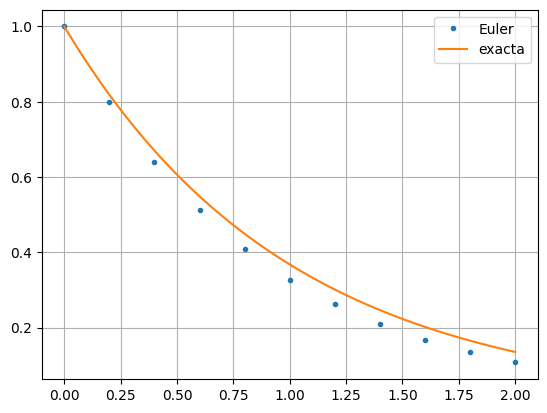
\includegraphics[width=0.6\linewidth]{Clase3_Practica2/euler_c3p2.png}
\end{figure}

\subsection{M\'etodo de Taylor de orden $k$}

$$y(x) \approx y(x_{0}) + y'(x_{0})(x - x_{0}) + y''(x_{0})\frac{(x - x_{0})^{2}}{2!} + \cdots + y^{k}(x_{0})\frac{(x - x_{0})^{k}}{k!} + \mathcal{O}((x - x_{0})^{k + 1})$$

Si $k = 1$, el m\'etodo de Taylor de orden 1 es Euler:

$$y(x) \approx y(x_{0}) + y'(x_{0})(x - x_{0}) = y(x_{0}) + f(x_{0}, y(x_{0}))$$

Si $k = 2$:

$$y(x) \approx y(x_{0}) + y'(x_{0})(x - x_{0}) + y''(x_{0})\frac{(x - x_{0})^{2}}{2!}$$

$$y'(x) = f(x, y(x)) \Rightarrow y''(x) = \frac{\partial f}{\partial x}(x, y(x))1 + \frac{\partial f}{\partial y}(x, y(x))y'(x) =  f_{x}(x, y(x)) + f_{y}(x, y(x))f(x, y(x))$$

Luego,

$$y(x) \approx y(x_{0}) + f(x_{0}, y(x_{0}))(x - x_{0}) + [f_{x}(x, y(x)) + f_{y}(x, y(x))f(x, y(x))]\frac{(x - x_{0})^{2}}{2!}$$

\subsection{M\'etodo de Taylor de orden 2 (general)}

$$ 
	\begin{cases}
        y_{i + 1} = y_{i} + f(x_{i}, y_{i})h + [f_{x}(x_{i}, y_{i}) + f_{y}(x_{i}, y_{i})f(x_{i}, y_{i})]\frac{h^{2}}{2!}\\
        y_{0} = y(x_{0})\\
    \end{cases}
$$

\textit{Ejemplo}:

$$ 
	\begin{cases}
        y'(t) = 2y(t) - 5\sin(t) = f(t, y(t))\\
        y(0) = 1\\
    \end{cases}
$$

Se resuelve Euler de la siguiente manera: $f(t, y) = 2y - 5\sin(t) \Rightarrow f(t_{i}, y_{i}) = 2y_{i} - 5\sin(t_{i})$.\\

$$ 
	\begin{cases}
        y_{i + 1} = y_{i} + h(2y_{i} - 5\sin(t_{i})),\ 0 \leq i \leq N\\
        y_{0} = 1\\
    \end{cases}
$$

Para Taylor de orden 2 (hay dos caminos):\\

$$ A = 
	\begin{cases}
        y_{i + 1} = y_{i} + h(2y_{i} - 5\sin(t_{i})) + \frac{h^{2}}{2!}(-5\cos(t_{i}) + 2(2y_{i} - 5\sin(t_{i})))\\
        y_{0} = 1\\
    \end{cases}
$$

$$ B = 
	\begin{cases}
        y_{i + 1} = y_{i} + h(2y_{i} - 5\sin(t_{i})) + \frac{h^{2}}{2!}(2(2y_{i} - 5\sin(t_{i})) - 5\cos(t_{i}))\\
        y_{0} = 1\\
    \end{cases}
$$\\

Con Taylor de orden $k$,

$$\phi(x_{i}, y_{i}, h) = T_{k}(x_{i}, y_{i}, h) = f(x_{i}, y_{i}) + f'(x_{i}, y_{i})\frac{h}{2} + \cdots + f^{k}(x_{i}, y_{i})\frac{h^{k - 1}}{k!}$$

\subsection{M\'etodos de Runge - Kutta}

$$y_{i + 1} = y_{i} + h\sum \limits_{j = 1}^{n} f(\theta_{j}, \eta_{j})A_{j}$$

donde $\theta_{j},\ \eta_{j}$ son puntos cercanos a $(x_{i}, y_{i})$. Vamos a considerar los m\'etodos de Runge - Kutta de la siguiente forma:

$$y_{i + 1} = y_{i} + h(A_{1}f(x_{i}, y_{i}) + A_{2}f(x_{i} + \alpha h, y_{i} + \beta hf(x_{i}, y_{i})))$$

Queremos algo parecido a Taylor pero sin tener que calcular derivadas de la funci\'on. Derivando el t\'ermino que acompa\~na a $A_{2}$ con respecto de $h$:

$$f(x_{i} + \alpha h, y_{i} + \beta hf(x_{i}, y_{i})) = f(x_{i}, y_{i}) + \frac{\partial f}{\partial x}(x_{i}, y_{i})\alpha h + \frac{\partial f}{\partial y}(x_{i}, y_{i})\beta f(x_{i}, y_{i})h + \mathcal{O}(h^{2})$$ 

Reemplazando en el m\'etodo:

$$y_{i + 1} = y_{i} + h(A_{1}f(x_{i}, y_{i}) + A_{2}[f(x_{i}, y_{i}) + f_{x}(x_{i}, y_{i})\alpha h + f_{y}(x_{i}, y_{i})\beta f(x_{i}, y_{i})h + \mathcal{O}(h^{2})])$$

Comparando con Taylor de orden 2 t\'ermino a t\'ermino (y tirando los t\'erminos de orden 3) nos queda $A_{1} + A_{2} = 1,\ A_{2}\alpha = \frac{1}{2},\ A_{2}\beta = \frac{1}{2}$.\\

Una primera elecci\'on, $\alpha = 1 \Rightarrow A_{2} = \frac{1}{2} = A_{1} \Rightarrow \beta = 1$, resulta el m\'etodo de Heun (RK2):

$$y_{i + 1} = y_{i} + \frac{h}{2}(f(x_{i}, y_{i}) + f(x_{i} + h, y_{i} + hf(x_{i}, y_{i}))) = y_{i} + \frac{h}{2}(K_{1} + K_{2})$$

La segunda elecci\'on, $\alpha = \frac{1}{2} \Rightarrow A_{2} = 1,\ A_{1} = 0 \Rightarrow \beta = \frac{1}{2}$, resulta el m\'etodo de Euler modificado (RK2):

$$y_{i + 1} = y_{i} + hf\bigg(x_{i} + \frac{h}{2}, y_{i} + \frac{h}{2}f(x_{i}, y_{i})\bigg)$$

El m\'etodo de Runge - Kutta 4 se define como:

$$y_{i + 1} = y_{i} + \frac{h}{6}(K_{1} + 2K_{2} + 2K_{3} + K_{4})$$

$$ 
	\begin{cases}
        K_{1} = f(x_{i}, y_{i})\\
        K_{2} = f(x_{i} + \frac{h}{2}, y_{i} + \frac{h}{2}K_{1})\\
        K_{3} = f(x_{i} + \frac{h}{2}, y_{i} + \frac{h}{2}K_{2})\\
        K_{4} = f(x_{i} + h, y_{i} + hK_{3})\\
    \end{cases}
$$
\newpage
\section{Clase 4 - Pr\'actica 2 (Ecuaciones diferenciales - Problema de valores iniciales)}

\subsection{Errores de truncado}

\underline{Definici\'on}: Dados $x^{*},\ h$, definimos el error de truncado local $\tau = \tau(x^{*})$ como:

$$y(x^{*} + h) = y(x^{*}) + h\phi(x^{*}, y(x^{*}), h) + h\tau$$

\textit{Ejemplo}: Si $\theta \in (x^{*}, x^{*} + h)$

\begin{itemize}
	\item Para Euler: $\tau = \frac{h}{2}y''(\theta)$
	
	\item Para Taylor de orden $k$: $\tau = \frac{h^{k}}{(k + 1)!}y^{k + 1}(\theta)$
\end{itemize}

\underline{Definici\'on}: Decimos que el m\'etodo de un paso tiene orden $p \in \mathbb{N}$ si $\tau = \mathcal{O}(h^{p})$, si suponemos que la soluci\'on tiene derivada de orden $p + 1$ acotada.\\

Euler es un m\'etodo de orden 1, Taylor 2 o RK2 son de orden 2, etc.\\

\underline{Definici\'on}: Decimos que el m\'etodo de un paso $y_{i + 1} = y_{i} + h\phi(x_{i}, y_{i}, h)$ converge si para cualquier $x^{*} \in [a, b],\ \lim \limits_{h \rightarrow \infty} y_{n} = y(x^{*})$.\\

\underline{Definici\'on}: Condici\'on CL. Decimos que $\phi(x, y, h)$ satisface la condici\'on CL si:

$$|\phi(x, u, h) - \phi(x, v, h)| \leq K|u - v|$$

con $x \in [a, b],\ 0 \leq h \leq b - a,\ u, v \in \mathbb{R}$. Luego, $\phi$ es Lipschitz respecto de su segunda variable.\\

\underline{Teorema}: Error global. Si $\phi$ satisface la condici\'on CL con constante $K$ y adem\'as $h = \frac{b - a}{n},\ x_{j} = a + hj,\ j = 0, \cdots, n$, entonces:

$$|E_{j}| = |y(x_{j}) - y_{j}| \leq \frac{\tau_{\max}}{K}(e^{K(x_{j} - x_{0})} - 1)$$

donde $\tau_{\max} = \max \limits_{0 \leq i \leq j} |\tau_{i}|$.\\

\underline{Demostraci\'on}:

$$y_{j + 1} = y_{j} + h\phi(x_{j}, y_{j}, h)$$

$$y(x_{j + 1}) = y(x_{j}) + h\phi(x_{j}, y_{j}(x_{j}), h) + h\tau_{j}$$

$$|E_{j + 1}| = |y(x_{j + 1}) - y_{j + 1}| = |y(x_{j}) - y_{j} + h\phi(x_{j}, y(x_{j}), h) - h\phi(x_{j}, y_{j}, h) + h\tau_{j}|$$

$$\leq |E_{j}| + h|\phi(x_{j}, y(x_{j}), h) \phi(x_{j}, y_{j}, h)| + h|\tau_{j}| \leq |E_{j}| + hK|E_{j}| + h\tau_{\max} = (1 + hK)|E_{j}| + h\tau_{\max}$$

$$\leq (1 + hK)[(1 + hK)|E_{j - 1}| + h\tau_{\max}] + h\tau_{\max} = (1 + hK)^{2}E_{j - 1} + (1 + hK)h\tau_{\max} + h\tau_{\max}$$

$$\leq (1 + hK)^{j + 1}|E_{j - 1}| + h\tau_{\max}\sum \limits_{l = 0}^{j} (1 + hK)^{l} = h\tau_{\max} \frac{(1 + hK)^{j + 1} - 1}{hK} = \frac{\tau_{\max}}{K}[(1 + hK)^{j - 1} - 1]$$

Como vale que $(1 + z)^{n} \leq e^{nz},\ z \in \mathbb{R}_{\geq 0}$, luego:

$$\frac{\tau_{\max}}{K}[(1 + hK)^{j - 1} - 1] \leq \frac{\tau_{\max}}{K}(e^{hK(j + 1)} - 1)$$

Caso particular: $|y_{N} - y_{0}| \leq \frac{\tau_{\max}}{K}(e^{K(x_{N} - x_{0})} - 1)$\\

C\'omo ver el orden de los m\'etodos en forma num\'erica?

$$E = \mathcal{O}(h^{p}) \approx \text{Error} = ch^{p}$$

$$\Rightarrow \log(\text{Error}) = \log(ch^{p}) = \log(c) + \log(h^{p}) = k + p\log(h) \Rightarrow y = k + px$$

El orden se ve como la pendiente de una recta.\\

\underline{Euler}: $\phi(x_{i}, y_{i}, h) = f(x_{i}, y_{i})$\\

La constante $K$ del teorema es la constante de Lipschitz de $f(x, y)$, $|f(x, u) - f(x, v)| \leq K|u - v|$

$$\tau_{i} = \frac{h}{2}y''(\theta)$$

es el error de truncado local para Euler, con $\theta \in (x_{i}, x_{i + 1})$.\\

Como $y' = f(x, y) \Rightarrow y'' = f'(x, y) = f_{x}(x, y) + f_{y}(x, y)y' = f_{x}(x, y) + f_{y}(x, y)f(x, y)$.\\

Sea $Y = \max \limits_{x \in [x_{0}, x_{N}]} |y''(x)| \Rightarrow |E_{N}| \leq \frac{h}{2K}Y(e^{K(x_{N} - x_{0})} - 1)$,

$$|y_{N} - y(x^{*})| \leq \frac{(x^{*} - a)}{2Kn}Y(e^{K(x_{N} - x_{0})} - 1) \rightarrow_{n \rightarrow +\infty} 0$$

Para que converja, $\tau$ tiene que tener un $h$. El m\'etodo de un paso converge si $\tau \rightarrow_{h \rightarrow 0} 0$.\\

\underline{Definici\'on}: Se dice que el m\'etodo de un paso es consistente si el error de truncado local $\tau \rightarrow_{h \rightarrow 0} 0$.\\

Ver consistencia es equivalente a ver que $\phi$ (continua en $h$) satisface $\phi(x_{i}, y(x_{i}), 0) = f(x_{i}, y(x_{i}))$. Lo que propongo como esquema aproxima a mi ecuaci\'on diferencial.\\

Para los m\'etodos de un paso, la consistencia implica la convergencia (por teorema): $\tau_{\max} \rightarrow_{h \rightarrow 0} 0$, entonces converge.\\

\textit{Ejemplo}: Considerar el problema de valores iniciales en $[0, 1]$:

$$ 
	\begin{cases}
        y'(t) = t\cos^{2}(y(t))\\
        y(0) = 5\\
    \end{cases}
$$

\begin{itemize}
	\item a) Escribir la iteraci\'on del m\'etodo de Euler correspondiente a este problema.
	
	$$ 
		\begin{cases}
        	y_{i + 1} = y_{i} + hf(t_{i}, y_{i})\\
        	y_{0} = 5\\
    	\end{cases}
	\Rightarrow
		\begin{cases}
        	y_{i + 1} = y_{i} + h(t_{i}\cos^{2}(y_{i}))\\
        	y_{0} = 5\\
    	\end{cases}
	$$
		
	con $0 \leq i \leq N - 1,\ h = \frac{t_{N} - t_{0}}{N} = \frac{1}{N}$\\
	
	\item b) Hallar $h$ para que el error al estimar $y(1)$ con el m\'etodo de Euler sea menor que $10^{-3}$.
	
	$$|y_{N} - y(1)| \leq \frac{\tau_{\max}}{K}(e^{K(1 - 0)} - 1)$$
	
	$\phi(t_{i}, y_{i}, h) = f(t, y) = t\cos^{2}(y)$. Quiero hallar $K$:
	
	$$|f(t, x) - f(t, y)| \leq K|x - y| \Rightarrow |t\cos^{2}(x) - t\cos^{2}(y)| = \bigg| \frac{\partial f}{\partial y}(t, \theta)\bigg||x - y| = |t2\cos(\theta)\sin(\theta)||x - y| \leq 2|x - y|$$
	
	Luego, $K = 2$ y nos queda:
	
	$$|y_{N} - y(1)| \leq \frac{\tau_{\max}}{2}(e^{2} - 1)$$

	En Euler, $|\tau_{i}| = \frac{h}{2}|y''(\theta)|,\ \theta \in (t_{i}, t_{i + 1})$. Hay dos formas de hallar esta derivada segunda:
	
	$$1^{\circ})\ y''(t) = 1\cos^{2}(y(t)) + t2\cos(y(t))(-\sin(y(t)))y'(t) = \cos^{2}(y(t)) - 2t\cos(y(t))\sin(y(t))t\cos^{2}(y(t))$$
	
	$$2^{\circ})\ y''(t) = \cos^{2}(y) + t2\cos(y)(-\sin(y))t\cos^{2}(y) = \frac{\partial f}{\partial t} + \frac{\partial f}{\partial y}f(t, y)$$

	Si acotamos $y''(t)$:
	
	$$|y''(t)| \leq |\cos^{2}(y)| + 2t^{2}|\cos^{3}(y)||\sin(y)| \leq 1 + 2 = 3$$
	
	pues $t \in [0, 1]$. Luego, $|\tau_{i}| \leq \frac{3}{2}h$, entonces:
	
	$$|y_{N} - y(1)| \leq \frac{3}{2}h\frac{1}{2}(e^{2} - 1) \leq 10^{-3}$$
	
	$$\Rightarrow h \leq \frac{10^{-3}}{6}$$
\end{itemize}

\textit{Python}: Euler

$$ 
	\begin{cases}
        y'(t) = y(t),\ t \in [0, 1]\\
        y(0) = 1\\
    \end{cases}
$$

\begin{verbatim}
	import numpy as np
	import matplotlib.pyplot as plt
	
	def f(t, y):
	    return y
		
	def Euler(a, b, f, y0):
	    h = [0.1, 0.0625, 0.05, 0.025, 0.01]
	    m = len(h)
	    logH = np.log(h)
	    ExactaEnUno = np.exp(1)
	    E = np.zeros(m)
		
	    for j in range(0, m):
	        N = int((b - a) / h[j])
	        t = np.linspace(a, b, N + 1)
	        y = np.zeros(N + 1)
	        y[0] = 1
	        
	        for i in range(0, N):
	            y[i + 1] = y[i] + h[j] * f(t[i], y[i])
	            
	        plt.plot(t, y)
	        AproxEnUno = y[N]
	        
	        E[j] = np.abs(ExactaEnUno - AproxEnUno)
	        
	    logE = np.log(E)
	    
	    Pendiente = np.abs((logE[m - 2] - logE[m - 1]) / (logH[m - 2] - logH[m - 1]))
		
	    return Pendiente
		
	a = 0
	b = 1
	y0 = 1
	
	Pendiente = Euler(a, b, f, y0)
	
	print(Pendiente)
	# 0.9852497002053401
\end{verbatim}

\begin{figure}[H]
  \centering
  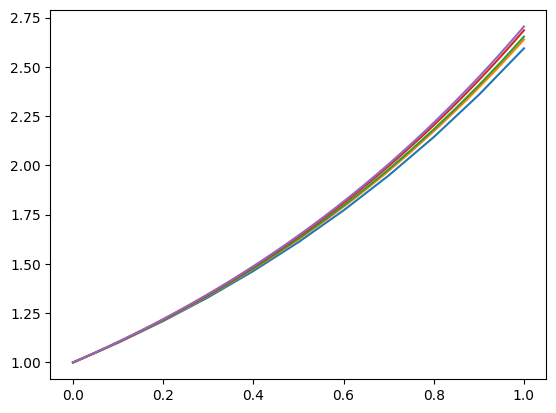
\includegraphics[width=0.6\linewidth]{Clase4_Practica2/euler_c4p2.png}
\end{figure}
\newpage
\section{Clase 5 - Pr\'actica 3 (Ecuaciones diferenciales - Problema de valores de contorno)}

\subsection{Diferencias finitas}

Partimos de un problema de valores de contorno

$$ 
	\begin{cases}
        u''(x) = p(x)u'(x) + q(x)u(x) + f(x)\\
        u(a) = \alpha,\ u(b) = \beta \\
    \end{cases}
$$

Buscamos $(u_{0}, \cdots, u_{N})$ de forma tal que $u_{j} \approx u(x_{j}),\ 1 \leq j \leq N - 1$.\\

\underline{Teorema}: Dada la ecuaci\'on de segundo orden $u''(x) = p(x)u'(x) + q(x)u(x) + f(x)$, con $a \leq x \leq b$ y valores en la frontera $u(a) = \alpha,\ u(b) = \beta$. Si $p, q, f$ son continuas en $[a, b]$ y $q > 0$, entonces el problema tiene soluci\'on \'unica.\\

Sea $N \in \mathbb{N}$, tomamos un paso $h = \frac{b - a}{N}$ y consideramos los puntos $x_{j} = a + jh$ con $j = 0, \cdots, N$ (notar que $x_{0} = a$ y $x_{N} = b$). Definimos $u_{0} = \alpha,\ u_{N} = \beta$ y aproximamos las derivadas de $u$.\\

\subsection{Discretizaciones usuales de $u'$}

$$\text{FORWARD}\ \ \ u'(x) \approx \frac{u(x_{j + 1}) - u(x_{j})}{h}$$

$$\text{BACKWARD}\ \ \ u'(x) \approx \frac{u(x_{j}) - u(x_{j - 1})}{h}$$

$$\text{CENTRADA}\ \ \ u'(x) \approx \frac{u(x_{j + 1}) - u(x_{j - 1})}{2h}$$

\subsection{Discretizaci\'on usual de $u''$}

$$u(x + h) = u(x) + hu'(x) + \frac{h^{2}}{2!}u''(x) + \frac{h^{3}}{3!}u'''(x) + \frac{h^{4}}{4!}u^{IV}(\zeta_{1})$$

$$u(x - h) = u(x) - hu'(x) + \frac{h^{2}}{2!}u''(x) - \frac{h^{3}}{3!}u'''(x) + \frac{h^{4}}{4!}u^{IV}(\zeta_{2})$$

$$\Rightarrow u(x + h) + u(x - h) = 2u(x) + h^{2}u''(x) + \frac{h^{4}}{4!}(u^{IV}(\zeta_{1}) + u^{IV}(\zeta_{2}))$$

$$u''(x) = \frac{u(x + h) - 2u(x) + u(x - h)}{h^{2}} - \frac{h^{2}}{4!}(u^{IV}(\zeta_{1}) + u^{IV}(\zeta_{2})) = \frac{u(x + h) - 2u(x) + u(x - h)}{h^{2}} - \mathcal{O}(h^{2})$$

Llamamos $p_{j} = p(x_{j}),\ q_{j} = q(x_{j}),\ f_{j} = f(x_{j})$ y usando diferencias centradas proponemos:

$$\frac{u_{j + 1} - 2u_{j} + u_{j - 1}}{h^{2}} = p_{j}\frac{u_{j + 1} - u_{j - 1}}{2h} + q_{j}u_{j} + f_{j}$$

Multiplicando por $h^{2}$ y reagrupando:

$$u_{j + 1} - 2u_{j} + u_{j - 1} - \frac{1}{2}hp_{j}(u_{j + 1} - u_{j - 1}) - h^{2}q_{j}u_{j} = h^{2}f_{j}$$

$$\bigg(1 + \frac{1}{2}hp_{j}\bigg)u_{j - 1} - (2 + h^{2}q_{j})u_{j} + \bigg(1 - \frac{1}{2}hp_{j}\bigg)u_{j + 1} = h^{2}f_{j}$$

\begin{itemize}
	\item $j = 1:\ -(2 + h^{2}q_{1})u_{1} + \bigg(1 - \frac{1}{2}hp_{1}\bigg)u_{2} = h^{2}f_{1} - \bigg(1 + \frac{1}{2}hp_{1} \bigg)u_{0},\ u_{0} = \alpha$
	
	\item $2\leq j \leq N - 2:\ \bigg(1 + \frac{1}{2}hp_{j}\bigg)u_{j - 1} - (2 + h^{2}q_{j})u_{j} + \bigg(1 - \frac{1}{2}hp_{j}\bigg)u_{j + 1} = h^{2}f_{j}$
	
	\item $j = N - 1:\ \bigg(1 + \frac{h}{2}p_{N - 1}\bigg)u_{N - 2} - (2 + h^{2}q_{N - 1})u_{N - 1} = h^{2}f_{N - 1} - \bigg(1 - \frac{h}{2}p_{N - 1}\bigg)u_{N},\ u_{N} = \beta$
\end{itemize}

En forma matricial: $A_{h}u_{h} = b_{h}$,

$$
    \begin{pmatrix}
        -(2 + h^{2}q_{1}) & (1 - \frac{1}{2}hp_{1}) & \cdots\\
        \cdots & \cdots & \cdots\\
        \vdots & \vdots & \vdots\\
        \cdots & (1 - \frac{1}{2}hp_{N - 1}) & -(2 + h^{2}q_{N - 1})\\

	\end{pmatrix}
    \begin{pmatrix}
        u_{1}\\
        \vdots\\
        \vdots\\
        u_{N - 1}\\
	\end{pmatrix}
	=
	\begin{pmatrix}
        h^{2}f_{1} - (1 + \frac{h}{2}p_{1})\alpha\\
        h^{2}f_{2}\\
        \vdots\\
        h^{2}f_{N - 1} - (1 + \frac{h}{2}p_{N - 1})\beta\\
	\end{pmatrix}
$$

\underline{Teorema 1}: Si $q > 0$ y $h < \frac{2}{M}$ con $M = \max \{|p(x)|,\ a < x < b\}$, la matriz es inversible.\\

\underline{Teorema 2}: Sea $A = \{a_{ij}\}_{i, j = 1, \cdots, N}\ / \ |a_{jj}| > \sum \limits_{k \neq j} |a_{jk}|$. Entonces todos los autovalores son distintos de 0.\\

\underline{Demostraci\'on}: Sea $\lambda$ cualquier autovalor y $v$ su autovector asociado. Sea $v_{j}$ la (o una) coordenada de mayor m\'odulo.\\

Si $w = \frac{v}{v_{j}},\ |w_{i}| = \bigg| \frac{v_{i}}{v_{j}}\bigg| \leq 1$ y $w_{i} = 1$ y $Aw = \lambda w$. Entonces, si miramos la fila $j$:

$$\sum \limits_{k \neq j} a_{jk}w_{k} + a_{jj} = \sum \limits_{k \neq j} a_{jk}w_{k} + a_{jj}w_{j} = \lambda w_{j} = \lambda$$

Si fuera $\lambda = 0$ tendr\'iamos $-a_{jj} = \sum \limits_{k \neq j} a_{jk}w_{k}$. Tomando m\'odulo, por desigualdad triangular, llegamos a un absurdo.

\subsection{Error de truncado local}

Volvemos al problema original:

$$\frac{u_{j + 1} - 2u_{j} + u_{j - 1}}{h^{2}} = p_{j}\frac{u_{j + 1} - u_{j - 1}}{2h} + q_{j}u_{j} + f_{j}$$

Si reemplazamos $u(x_{j})$ por $u_{j}$ en la ecuaci\'on de diferencias, obtenemos:

$$\frac{u(x_{j + 1}) - 2u(x_{j}) + u(x_{j - 1})}{h^{2}} = p_{j}\frac{u(x_{j + 1}) - u(x_{j - 1})}{2h} + q_{j}u(x_{j}) + f_{j} + \tau_{j}$$

Pero vimos que:

$$\frac{u(x_{j} + h) - 2u(x_{j}) + u(x_{j} - h)}{h^{2}} = u''(x_{j}) + \mathcal{O}(h^{2})$$

$$\frac{u(x_{j} + h) - u(x_{j} - h)}{2h} = u'(x_{j}) + \mathcal{O}(h^{2})$$

Reemplazamos y reagrupamos:

$$u''(x_{j}) + \mathcal{O}(h^{2}) = p_{j}(u'(x_{j}) + \mathcal{O}(h^{2})) + q_{j}u(x_{j}) + f_{j} + \tau_{j}$$

$$\Rightarrow u''(x_{j}) + \mathcal{O}(h^{2}) = p_{j}u'(x_{j}) + p_{j}\mathcal{O}(h^{2}) + q_{j}u(x_{j}) + f_{j} + \tau_{j}$$

Pero la soluci\'on verdadera $u$ cumple:

$$u''(x_{j}) = p_{j}u'(x_{j}) + q_{j}u(x_{j}) + f_{j}$$

$$\Rightarrow \tau_{j} = \mathcal{O}(h^{2})$$

Tenemos dos ecuaciones, una para $u$ y otra para $u_{h}$:

$$A_{h}u_{h} = b_{h}$$
$$A_{h}u = b_{h} + \tau_{h}$$

donde $\tau_{h}$ es el vector de error de truncado, entonces $(u - u_{h}) = A_{h}^{-1}\tau_{h}$.\\

\underline{Teorema}: Si existe $A_{h}^{-1},\ \|A_{h}^{-1}\| \leq C,\ \forall \ h$ suficientemente chico (es decir, el m\'etodo es estable) y $\tau_{h} \rightarrow 0$ (es decir, el m\'etodo es consistente), entonces $\|u - u_{h}\| \rightarrow 0$ (el m\'etodo converge).

\subsection{Ecuaciones de evoluci\'on en derivadas parciales}

\textit{Ejemplo}: Ecuaci\'on de calor

$$ 
	\begin{cases}
        u_{t}(x, t) = \alpha u_{xx}(x, t),\ x \in (0, L),\ t > 0\\
        u(x, 0) = g(x),\ x \in [0, L]\\
        u(0, t) = u(L, t) = 0,\ t > 0\\
    \end{cases}
$$

Consideramos $\alpha = 1$. Vamos a discretizar el dominio $x_{j} = jh,\ h = \Delta x = \frac{L}{J},\ t_{n} = nk,\ k = \Delta t = \frac{T_{F}}{N}$. Queremos aproximar $u(x_{j}, t_{n}) \approx u_{j}^{n}$. Con la discretizaci\'on usual de la derivada segunda y diferencias forward para la primera, tenemos:

$$ 
	\begin{cases}
		\frac{u_{j}^{n + 1} - u_{j}^{n}}{k} = \frac{u_{j + 1}^{n} - 2u_{j}^{n} + u_{j - 1}^{n}}{h^{2}},\ 1 \leq j \leq J - 1,\ 1 \leq n \leq N - 1\\
		u_{j}^{0} = g(x_{j}),\ 0 \leq j \leq J\\
		u_{0}^{n} = u_{J}^{n},\ 0 \leq n \leq N\\
    \end{cases}
$$

Podemos despejar:

$$u_{j}^{n + 1} = \frac{k}{h^{2}}u_{j - 1}^{n} + \bigg(1 - \frac{2k}{h^{2}}\bigg)u_{j}^{n} + \frac{k}{h^{2}}u_{j + 1}^{n}$$

\begin{itemize}
	\item $j = 1:\ u_{j}^{n + 1} = 0 + \bigg(1 - \frac{2k}{h^{2}}\bigg)u_{1}^{n} + \frac{k}{h^{2}}u_{2}^{n}$
	
	\item $2\leq j \leq J - 2:\ u_{j}^{n + 1} = \frac{k}{h^{2}}u_{j - 1}^{n} + \bigg(1 - \frac{2k}{h^{2}}\bigg)u_{j}^{n} + \frac{k}{h^{2}}u_{j + 1}^{n}$
	
	\item $j = J - 1:\ u_{J - 1}^{n + 1} = \frac{k}{h^{2}}u_{J - 2}^{n} + \bigg(1 - \frac{2k}{h^{2}}\bigg)u_{J - 1}^{n} + 0$
\end{itemize}

$$
	\begin{pmatrix}
        u_{1}^{n + 1}\\
        \vdots\\
        \vdots\\
        u_{J - 1}^{n + 1}\\
	\end{pmatrix}
	=
    \begin{pmatrix}
        1 - \frac{2k}{h^{2}} & \frac{k}{h^{2}} & \cdots\\
        \frac{k}{h^{2}} & \cdots & \cdots\\
        \vdots & \vdots & \vdots\\
        \cdots & \cdots & \cdots\\

	\end{pmatrix}
    \begin{pmatrix}
        u_{1}^{n}\\
        \vdots\\
        \vdots\\
        u_{J - 1}^{n}\\
	\end{pmatrix}
$$

El error de truncado se obtiene al reemplazar la soluci\'on num\'erica por la real en el esquema, es decir:

$$\frac{u(x, t + k) - u(x, t)}{k} = \frac{u(x + h, t) - 2u(x, t) + u(x - h, t)}{h^{2}} + \tau$$

donde $\tau$ es el error de truncado.\\

\textit{Python}: Diferencias finitas

$$ 
	\begin{cases}
        -\alpha u''(x) = f(x) = \sin(\pi x)\\
        u(0) = u(1) = 0\\
    \end{cases}
$$

\begin{verbatim}
	import numpy as np
	import matplotlib.pyplot as plt
	
	def f(x):
	    return np.sin(np.pi * x)
		
	def DifFinitas(a, b, alpha, h, f):
	    N = int((b - a) / h)
	    t = np.linspace(a, b, N + 1)
	    u = np.zeros(N + 1)
	    b = np.zeros(N + 1)
		
	    for i in range(1, N):
	        b[i - 1] = f(t[i])
	        
	    Diag = np.ones(N - 1) * (2 * alpha / (h**2))
	    DiagArriba = np.ones(N - 2) * (-alpha / (h**2))
	    
	    A = np.diag(Diag) + np.diag(DiagArriba, 1) + np.diag(DiagArriba, -1)
		
	    u = np.linalg.solve(A, b)
	    
	    return (t, u)
		
	a = 0
	b = 1
	alpha = 1
	h = 0.01
	
	t, Solucion = DifFinitas(a, b, alpha, h, f)
	
	print(Solucion)
	
	# A la solucion debo agregarle los bordes que eran datos
	SolucionBD = np.append(Solucion, 0)
	
	print(SolucionBD)
	
	SolucionBIBD = np.append(0, SolucionBD)
	
	print(SolucionBIBD)
	
	plt.plot(t, SolucionBIBD)
\end{verbatim}

\begin{figure}[H]
  \centering
  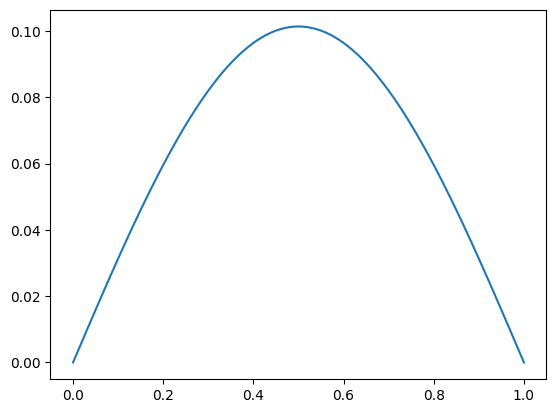
\includegraphics[width=0.6\linewidth]{Clase5_Practica3/difs_c5p3.png}
\end{figure}
\newpage
\section{Clase 6 - Pr\'actica 3 (Ecuaciones diferenciales - Problema de valores de contorno)}

\underline{Definici\'on 1}: Decimos que el m\'etodo es consistente si $T \rightarrow_{h \rightarrow 0,\ k \rightarrow 0} 0$.\\

\underline{Definici\'on 2}: Decimos que el m\'etodo es estable en norma $\|.\|$ si existe una constante $C > 0$ (independiente de $h, k, j, n, J, N$) tal que $\|u^{n}\| \leq C\|u^{0}\|$.\\

Veamos cuando este m\'etodo es estable en norma $\infty$, $\|v\|_{\infty} = \max \limits_{j} \{|v_{j}|\}$.

$$\|u^{n + 1}\|_{\infty} = \max \limits_{j} \bigg\{\bigg| \frac{k}{h^{2}}u_{j - 1}^{n} + \bigg(1 - \frac{2k}{h^{2}}u_{j}^{n}\bigg) +  \frac{k}{h^{2}}u_{j + 1}^{n} \bigg| \bigg\} \leq \max \limits_{j} \bigg\{\bigg| \frac{k}{h^{2}}\|u_{j - 1}^{n}\|_{\infty} + \bigg|1 - \frac{2k}{h^{2}}\bigg|\|u_{j}^{n}\|_{\infty} +  \frac{k}{h^{2}}\|u_{j + 1}^{n}\|_{\infty} \bigg\}$$

$$\Rightarrow \|u^{n + 1}\|_{\infty} \leq \bigg(\frac{2k}{h^{2}} +   \bigg|1 - \frac{2k}{h^{2}}\bigg|\bigg)\|u^{n}\|_{\infty}$$

Si $\frac{2k}{h^{2}} < 1$, o sea, $2k < h^{2},\ \|u^{n + 1}\|_{\infty} \leq \|u^{n}\|_{\infty}$. Con este razonamiento concluimos $\|u^{n + 1}\|_{\infty} \leq \|u^{0}\|_{\infty}$ y el m\'etodo resulta estable con $C = 1$.\\

\underline{Error}:

$$u(x_{j}, t_{n + 1}) = \frac{k}{h^{2}}u(x_{j - 1}, t_{n}) + \bigg(1 - \frac{2k}{h^{2}}\bigg)u(x_{j}, t_{n}) + \frac{k}{h^{2}}u(x_{j - 1}, t_{n})+ k\tau_{j}^{n}$$

$$u_{j}^{n + 1} = \frac{k}{h^{2}}u_{j - 1}^{n} + \bigg(1 - \frac{2k}{h^{2}}\bigg)u_{j}^{n} + \frac{k}{h^{2}}u_{j + 1}^{n}$$

$$\Rightarrow e_{j}^{n + 1} = u(x_{j}, t_{n + 1}) - u_{j}^{n + 1} = \frac{k}{h^{2}}e_{j - 1}^{n} + \bigg(1 - \frac{2k}{h^{2}}\bigg)e_{j}^{n} + \frac{k}{h^{2}}e_{j + 1}^{n} + k\tau_{j}^{n}$$

\underline{Definici\'on 3}: Decimos que el m\'etodo es convergente si $\max \limits_{j, n} e_{j}^{n} \rightarrow_{h \rightarrow 0,\ k \rightarrow 0} 0$.\\

Llamamos $e^{n} = \max \limits_{j} \{|e_{j}^{n}|\}$ y $\tau^{n} = \max \limits_{j} \{|\tau_{j}^{n}|\}$, entonces

$$|e_{j}^{n + 1}| \leq \frac{k}{h^{2}}|e_{j - 1}^{n}| + \bigg|1 - \frac{2k}{h^{2}}\bigg||e_{j}^{n}| + \frac{k}{h^{2}}|e_{j}^{n}| + k|\tau_{j}^{n}|$$

$$|e_{j}^{n + 1}| \leq \frac{k}{h^{2}}e^{n} + \bigg|1 - \frac{2k}{h^{2}}\bigg|e^{n} + \frac{k}{h^{2}}e^{n} + k\tau^{n}$$

$$|e_{j}^{n + 1}| \leq e^{n} + k\tau^{n}$$

$$e^{n + 1} \leq e^{n} + k\tau^{n} \leq e^{0} + (k\tau^{0} + \cdots + k\tau^{n}) \leq (k\tau^{0} + \cdots + k\tau^{n}) = k \sum \limits_{i = 0}^{n} \tau^{i} \leq k(n + 1) \max \limits_{i} \max \limits_{j} |\tau_{i}^{j}|,\ n \leq N - 1$$

$$\Rightarrow e^{n + 1} \leq k(n + 1)[\mathcal{O}(k) + \mathcal{O}(h^{2})] \leq kN[\mathcal{O}(k) + \mathcal{O}(h^{2})] = T_{F}[\mathcal{O}(k) + \mathcal{O}(h^{2})],\ k = \frac{T_{F}}{N}$$

y el m\'etodo resulta convergente cuando $h \rightarrow 0,\ k \rightarrow 0$.\\

\begin{itemize}
	\item Notemos que si $h = 10^{-3}$, estamos pidiendo $2k < 10^{-6}$, es decir, $2\cdot10^{6} < N$.
\end{itemize}

Veamos un m\'etodo impl\'icito

$$ 
	\begin{cases}
		\frac{u_{j}^{n + 1} - u_{j}^{n}}{k} = \frac{u_{j + 1}^{n} - 2u_{j}^{n} + u_{j - 1}^{n}}{h^{2}},\ 1 \leq j \leq J - 1,\ 1 \leq n \leq N - 1\\
		u_{j}^{0} = g(x_{j}),\ 0 \leq j \leq J\\
		u_{0}^{n} = u_{J}^{n},\ 0 \leq n \leq N\\
    \end{cases}
$$

Despejamos: 

$$u_{j}^{n + 1} = -\frac{k}{h^{2}}u_{j - 1}^{n} + \bigg(1 + \frac{2k}{h^{2}}\bigg)u_{j}^{n} - \frac{k}{h^{2}}u_{j + 1}^{n}$$

Forma matricial:

$$
	\begin{pmatrix}
        u_{1}^{n + 1}\\
        \vdots\\
        \vdots\\
        u_{J - 1}^{n + 1}\\
	\end{pmatrix}
	=
    \begin{pmatrix}
        1 + \frac{2k}{h^{2}} & -\frac{k}{h^{2}} & \cdots\\
        -\frac{k}{h^{2}} & \cdots & \cdots\\
        \vdots & \vdots & \vdots\\
        \cdots & \cdots & \cdots\\

	\end{pmatrix}
    \begin{pmatrix}
        u_{1}^{n}\\
        \vdots\\
        \vdots\\
        u_{J - 1}^{n}\\
	\end{pmatrix}
$$

y debemos resolver el sistema lineal $A^{-1}u^{n} = u^{n + 1}$.\\

Verificar que vale:

\begin{itemize}
	\item $\tau = \mathcal{O}(k) + \mathcal{O}(h^{2})$

	\item $\bigg(1 + \frac{2k}{h^{2}}\bigg)e_{j}^{n + 1} = e_{j}^{n} + \frac{k}{h^{2}}e_{j - 1}^{n + 1} + \frac{k}{h^{2}}e_{j + 1}^{n + 1} + k\tau_{j}^{n + 1}$
\end{itemize}

Luego,

$$\bigg(1 + \frac{2k}{h^{2}}\bigg)|e_{j}^{n + 1}| \leq |e_{j}^{n}| + \frac{k}{h^{2}}|e_{j - 1}^{n + 1}| + \frac{k}{h^{2}}|e_{j + 1}^{n + 1}| + k|\tau_{j}^{n + 1}| \leq e^{n} + \frac{k}{h^{2}}e^{n + 1} + \frac{k}{h^{2}}e^{n + 1} + k\tau^{n + 1}$$

$$\Rightarrow e^{n + 1} \leq e^{n} + k\tau^{n + 1} \leq e^{n - 1} + k\tau^{n} + k\tau^{n + 1} \leq e^{0} + k(\tau^{1} + \cdots + \tau^{n + 1}) \leq k \sum \limits_{j = 1}^{n} \tau^{j} \leq k(n + 1) \max \limits_{i} \max \limits_{j} |\tau_{i}^{j}|$$

$$\Rightarrow e^{n + 1} \leq T_{F}[\mathcal{O}(k) + \mathcal{O}(h^{2})],\ n \leq N - 1$$

Cu\'al es la diferencia con el m\'etodo expl\'icito? En el m\'etodo impl\'icito NO necesitamos la condici\'on $2k < h^{2}$.\\

\textit{Python}: Diferencias finitas. Ecuaci\'on del calor

$$ 
	\begin{cases}
        u_{t}(x, t) = \alpha u_{xx}(x, t),\ x \in (0, 1)\\
        u(x, 0) = g(x) = \sin(\pi x),\ t \in [0, 1]\\
        u(0, t) = u(1, t) = 0,\ t > 0\\
    \end{cases}
$$

\begin{verbatim}
	import numpy as np
	import matplotlib.pyplot as plt
	
	def g(x):
	    return np.sin(np.pi * x)
		
	def DifFinitasCalor(x0, xf, t0, tf, alpha, DeltaX, DeltaT, g):
	    N = int((xf - x0) / DeltaX)
	    x = np.linspace(x0, xf, N + 1)
	    M = int((tf - t0) / DeltaT)
	    t = np.linspace(t0, tf, N + 1)
	    
	    u = np.zeros((M + 1, N + 1))
	    
	    u[0, :] = g(x)
	    
	    r = DeltaT / (DeltaX**2)
		
	    Diag = np.ones(N - 1) * (1 - 2 * alpha * r)
	    DiagArriba = np.ones(N - 2) * (alpha * r)
	    
	    A = np.diag(Diag) + np.diag(DiagArriba, 1) + np.diag(DiagArriba, -1)
	    
	    for i in range(1, M + 1):
	        u[i, 1:N] = A@u[i - 1, 1:N]
	    
	    return (t, u)
		
	x0 = 0
	xf = 1
	t0 = 0
	tf = 10
	alpha = 1
	DeltaX = 0.1
	DeltaT = 0.001
	
	t, u = DifFinitasCalor(x0, xf, t0, tf, alpha, DeltaX, DeltaT, g)
	
	print(t)
	print(u)
	
	M = int((tf - t0) / DeltaT)
	N = int((xf - x0) / DeltaX)
	
	x = np.linspace(x0, xf, N + 1)
	
	for i in range(0, M):
	    plt.plot(x, u[i, :])
\end{verbatim}

\begin{figure}[H]
  \centering
  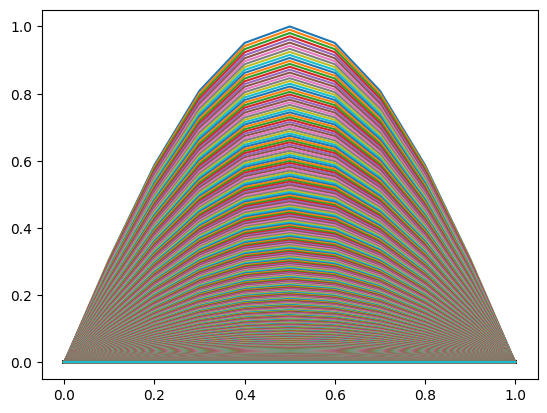
\includegraphics[width=0.6\linewidth]{Clase6_Practica3/difs_c6p3.png}
\end{figure}
\newpage
\section{Clase 7 - Pr\'actica 4 (N\'umero de condici\'on)}

\subsection{Normas vectoriales}

\begin{itemize}
	\item $\|x\|_{2} = \sqrt{x_{1}^{2} + \cdots + x_{n}^{2}}$
	
	\item $\|x\|_{\infty} = \max \limits_{1 \leq i \leq n} |x_{i}|$

	\item $\|x\|_{1} = \max \limits_{1 \leq j \leq n} |x_{j}|$

	\item $\|x\|_{p} = (x_{1}^{p} + \cdots + x_{n}^{p})^{\frac{1}{p}}$
\end{itemize}

\subsection{Desigualdad de Cauchy - Schwarz}

$$\langle a, b \rangle \leq \|a\|_{2}\|b\|_{2}$$

\underline{Demostraci\'on}: Basta probar que $\langle a, b \rangle^{2}\leq \|a\|_{2}^{2}\|b\|_{2}^{2}$ para $a \neq 0$.

$$0 \leq \|\alpha a - \beta b\|_{2}^{2} = \langle \alpha a - \beta b, \alpha a - \beta b \rangle = \alpha^{2}\|a\|_{2}^{2} - 2\alpha \beta \langle a, b \rangle + \beta^{2}\|b\|_{2}^{2}$$

Si tomamos $\alpha = \langle a, b \rangle$ y $\beta = \|a\|_{2}^{2}$:

$$0 \leq \|a\|_{2}^{2}\langle a, b \rangle^{2} - 2\|a\|_{2}^{2}\langle a, b \rangle^{2} + \|a\|_{2}^{4}\|b\|_{2}^{2} \Rightarrow \|a\|_{2}^{2}\langle a, b \rangle^{2} \leq \|a\|_{2}^{4}\|b\|_{2}^{2} \Rightarrow \langle a, b \rangle^{2} \leq \|a\|_{2}^{2}\|b\|_{2}^{2}$$

\underline{C\'omo se comparan las normas entre s\'i?}\\

Si tomamos $a = (|x_{1}|, \cdots, |x_{n}|),\ b = (1, \cdots, 1)$ por Cauchy - Schwarz.

$$\sum \limits_{1 \leq j \leq n} |x_{j}| = \langle a, b \rangle \leq \|a\|_{2}\|b\|_{2} = \sqrt{n}\|x\|_{2}$$

por lo tanto, $\|x\|_{1} \leq \sqrt{n}\|x\|_{2}$. Vale tambi\'en que

\begin{itemize}
	\item $\|x\|_{2} \leq \|x\|_{1}$

	\item $\|x\|_{\infty} \leq \|x\|_{1} \leq n\|x\|_{\infty}$
	
	\item $\|x\|_{\infty} \leq \|x\|_{2} \leq \sqrt{n}\|x\|_{\infty}$\\
\end{itemize}

\underline{Definici\'on}: Sea $V$ un espacio vectorial. Una norma en $V$ es una aplicaci\'on $\|.\|: V \rightarrow \mathbb{R}$ tal que:

\begin{itemize}
	\item 1) $\|x\| \geq 0\ \forall \ x \in V$
	
	\item 2) $\|x\| = 0 \iff x = 0$
	
	\item 3) $\|\lambda x\| = |\lambda|\|x\|$
	
	\item 4) $\|x + y\| \leq \|x\| + \|y\|$\\
\end{itemize}

\underline{Teorema}: Dadas $\|.\|$ y $\|.\|'$ normas en $\mathbb{R}^{n}$, existen constantes positivas $C_{1}$ y $C_{2}\ / \ C_{1}\|x\| \leq \|x\|' \leq C_{2}\|x\|$.\\

\underline{Demostraci\'on}: Basta demostrar que cualquier norma es equivalente a $\|.\|_{2}$.\\

Sea $e_{i}$ el $i$-\'esimo vector can\'onico. Llamemos $C = \bigg(\sum \limits_{i = 1}^{n} \|e_{i}\|'^{2}\bigg)^{\frac{1}{2}}$:

$$\|x\|' = \bigg\|\sum \limits_{j = 1}^{n} x_{j}e_{j}\bigg\|' \leq \sum \limits_{j = 1}^{n} |x_{j}|\|e_{j}\|' = \langle (|x_{1}|, \cdots, |x_{n}|), (\|e_{1}\|', \cdots, \|e_{n}\|') \rangle$$

Por la desigualdad de Cauchy - Schwarz, vale $\|x\|' \leq \|x\|_{2} \Rightarrow \frac{1}{C}\|x\|' \leq \|x\|_{2}$.\\

Consideramos $C_{1} = \frac{1}{C}$. Queremos ver ahora que existe $C_{2}\ / \ \|x\|_{2} \leq C_{2}\|x\|'$.\\

Supongamos que no, entonces $\forall \ m \in \mathbb{N}\ \exists \ y_{m} \in \mathbb{R}^{n}\ / \ \|y_{m}\|_{2} > m \|y_{m}\|'$.\\

Sea $z_{m} = \frac{y_{m}}{\|y_{m}\|_{2}}$, y por lo tanto:

$$\|z_{m}\|_{2} = 1 \text{ y } \|z_{m}\|' = \frac{1}{\|y_{m}\|_{2}}\|y_{m}\|' \leq \frac{1}{m} \rightarrow_{m \rightarrow +\infty} 0$$

Como $\{z_{m}\}$ es acotada en $\|.\|_{2}$, existe una subsucesi\'on convergente $\{z_{m_{k}}\|_{k}$ y $z \in \mathbb{R}^{n}\ / \ \|z_{m_{k}} - z\|_{2} \rightarrow_{k \rightarrow +\infty} 0$.\\

Vale entonces que $\|z_{m_{k}} - z\|' \leq C\|z_{m_{k}} - z\|_{2} \rightarrow_{k \rightarrow +\infty} 0$ y $0 \leq \|z\|' \leq \|z - z_{m_{k}}\|' + \|z_{m_{k}}\|' \rightarrow_{k \rightarrow +\infty} 0$. Por lo tanto, $z = 0$ pero $\|z_{m_{k}}\|_{2} = 1\ \forall \ k$ y esto lleva a un absurdo.\\

Si tengo una matriz $A$ y un vector $b$ y resuelvo el sistema $Ax = b$, obteniendo $x$. Ahora tengo el vector $\tilde{b}$ y obtengo $\tilde{x}$, c\'omo se comparan $\frac{\|x - \tilde{x}\|'}{\|x\|'}$ y $\frac{\|b - \tilde{b}\|'}{\|b\|'}$?\\

\textit{Ejemplo}:

$$ A = 
	\begin{pmatrix}
        4.1 & 2.8\\
        9.7 & 6.6\\
	\end{pmatrix}
	,\ b = 
    \begin{pmatrix}
        4.1\\
        9.7\\
	\end{pmatrix}
	,\ x = 
    \begin{pmatrix}
        1\\
        0\\
	\end{pmatrix}
	,\ \tilde{b} =
	\begin{pmatrix}
        4.11\\
        9.7\\
	\end{pmatrix}
	,\ \tilde{x} =
	\begin{pmatrix}
        0.34\\
        0.97\\
	\end{pmatrix}
$$

$$\frac{\|x - \tilde{x}\|_{1}}{\|x\|_{1}} = \frac{0.66 + 0.97}{1} = 1.63$$

$$\frac{\|b - \tilde{b}\|_{1}}{\|b\|_{1}} = \frac{0.01}{13.8} = 0.7246\cdot10^{-3}$$

\underline{Definici\'on}: Sea $A \in \mathbb{R}^{n \times n}$, definimos a la norma de $A$ subordinada a la norma vectorial $\|.\|'$
como:

$$\|A\|' = \max \limits_{x \neq 0} \frac{\|Ax\|'}{\|x\|'}$$

Equivalentemente, $\|A\|' = \max \limits_{\|x\|' = 1} \|Ax\|'$ (ver que es una norma).\\

\underline{Propiedades}:

\begin{itemize}
	\item $\|Ax\|' \leq \|A\|'\|x\|'$
	
	\item $\|AB\|' \leq \|A\|'\|B\|'$\\
	
	\underline{Demostraci\'on}: $\|ABx\|' \leq \|A\|'\|Bx\|' \leq \|A\|'\|B\|'\|x\|' \ \forall \ x$. Por lo tanto:
	
	$$\|AB\|' = \max \limits_{x \neq 0} \frac{\|ABx\|'}{\|x\|'} \leq \max \limits_{x \neq 0} \frac{\|A\|'\|B\|'\|x\|'}{\|x\|'} = \max \limits_{x \neq 0} \|A\|'\|B\|' = \|A\|'\|B\|'$$

\end{itemize}

\underline{Teorema}: Sea $A \in \mathbb{R}^{n \times n}$,

\begin{itemize}
	\item 1) $\|A\|_{\infty} = \max \limits_{1 \leq i \leq n} \sum \limits_{j = 1}^{n} |a_{ij}|$
	
	\item 2) Si $A$ es sim\'etrica y $\{\lambda_{1}, \cdots, \lambda_{n}\}$ son sus autovalores, $\|A\|_{2} = \rho(A) = \max \limits_{1 \leq j \leq n} |\lambda_{j}|$.
	
	Si $A$ no es sim\'etrica, $\|A\|_{2} = \sqrt{\rho(A^{t}A)}$
	
	\item 3) $\|A\|_{1} = \max \limits_{1 \leq j \leq n} \sum \limits_{i = 1}^{n} |a_{ij}|$
\end{itemize}

\underline{Demostraci\'on}:

\begin{itemize}
	\item 1)
	$\leq$:

	$$\|Ax\|_{\infty} = \max \limits_{1 \leq i \leq n} \bigg|\sum \limits_{j = 1}^{n} a_{ij}x_{j}\bigg|  \leq \max \limits_{1 \leq i \leq n} \sum \limits_{j = 1}^{n} |a_{ij}||x_{j}| \leq \max \limits_{1 \leq i \leq n} \|x\|_{\infty} \sum \limits_{j = 1}^{n} |a_{ij}|$$

	$$\Rightarrow \|A\|_{\infty} = \max \limits_{x \neq 0} \frac{\|Ax\|_{\infty}}{\|x\|_{\infty}} \leq \max \limits_{x \neq 0} \frac{\max \limits_{1 \leq i \leq n} \|x\|_{\infty} \sum \limits_{j = 1}^{n} |a_{ij}|}{\|x\|_{\infty}} = \max \limits_{1 \leq i \leq n} \sum \limits_{j = 1}^{n} |a_{ij}|$$
	
	$\geq$:
	
	Sea $i_{0}$ el \'indice donde se alcanza el m\'aximo. Es decir:
	
	$$\max \limits_{1 \leq i \leq n} \sum \limits_{j = 1}^{n} |a_{ij}| = \sum \limits_{j = 1}^{n} |a_{i_{0}j}|$$
	
	Sea $\tilde{x} = (\text{sg}(a_{i_{0}1}), \cdots, \text{sg}(a_{i_{0}n}))$. Vale $\|\tilde{x}\|_{\infty} = 1$.
	
	$$\|A\tilde{x}\|_{\infty} = \max \limits_{1 \leq i \leq n} \bigg|\sum \limits_{j = 1}^{n} a_{ij}\tilde{x}_{j}\bigg|  \geq \bigg|\sum \limits_{j = 1}^{n} a_{i_{0}j}\tilde{x}_{j}\bigg| = \bigg|\sum \limits_{j = 1}^{n} |a_{i_{0}j}|\bigg| = \sum \limits_{j = 1}^{n} |a_{i_{0}j}| = \max \limits_{1 \leq i \leq n} \sum \limits_{j = 1}^{n} |a_{ij}|$$
	
	$$\Rightarrow \|A\|_{\infty} = \max \limits_{x \neq 0} \frac{\|Ax\|_{\infty}}{\|x\|_{\infty}} \geq \frac{\|A\tilde{x}\|_{\infty}}{\|\tilde{x}\|_{\infty}} \geq \max \limits_{1 \leq i \leq n} \sum \limits_{j = 1}^{n} |a_{ij}|$$
	
	\item 2)
	$\leq$:
	
	Sea $A$ sim\'etrica. Existe una B.O.N. de autovectores (norma $\|.\|_{2}$). Sea $\lambda_{1}, \cdots, \lambda_{n}$ los autovalores de $A$ y $v_{1}, \cdots, v_{n}$ los autovectores asociados tales que $\langle v_{i}, v_{j} \rangle = \delta_{ij}$.\\
	
	Sea $x \in \mathbb{R}^{n}$. Entonces, $x = \sum \limits_{j = 1}^{n} \alpha_{j}v_{j}$ y $\|x\|_{2}^{2} = \sum \limits_{j = 1}^{n} \alpha_{j}^{2}$. Luego, $Ax = \sum \limits_{j = 1}^{n} \alpha_{j}Av_{j} = \sum \limits_{j = 1}^{n} \alpha_{j}\lambda_{j}v_{j}$:
	
	$$\|Ax\|_{2}^{2} = \sum \limits_{j = 1}^{n} (\alpha_{j}\lambda_{j})^{2} \leq \sum \limits_{j = 1}^{n} \alpha_{j}^{2}\lambda_{\max}^{2} = \lambda_{\max}^{2}\sum \limits_{j = 1}^{n} \alpha_{j}^{2} = \lambda_{\max}^{2}\|x\|_{2}^{2}$$
	
	$$\Rightarrow \|A\|_{2} = \max \limits_{x \neq 0} \frac{\|Ax\|_{2}}{\|x\|_{2}} \leq \frac{|\lambda_{\max}|\|x\|_{2}^{2}}{\|x\|_{2}} = |\lambda_{\max}| = \rho(A)$$
	
	$\geq$:
	
	Sea $i_{0}\ / \ \lambda_{\max} = \lambda_{i_{0}}$:
	
	$$\frac{\|Av_{i_{0}}\|_{2}}{\|v_{i_{0}}\|_{2}} = \frac{\|\lambda_{i_{0}}v_{i_{0}}\|_{2}}{\|v_{i_{0}}\|_{2}} = |\lambda_{i_{0}}| = \rho(A)$$
	
	$$\Rightarrow \|A\|_{2} \geq \rho(A)$$
	
	$\leq$:
	
	Si $A$ no es sim\'etrica, $B = A^{t}A$ s\'i lo es. Sean $\mu_{1}, \cdots, \mu_{n}$ los autovalores de $B$ (que no son negativos) y $w_{1}, \cdots, w_{n}$ los autovectores asociados que forman una B.O.N.\\
	
	Sea $x \in \mathbb{R}^{n}$. Entonces $x = \sum \limits_{j = 1}^{n} \alpha_{j}w_{j}$ y $Bx = \sum \limits_{j = 1}^{n} \alpha_{j}\mu_{j}w_{j}$:
	
	$$\|Ax\|_{2}^{2} = \langle Ax, Ax \rangle = x^{t}A^{t}Ax = x^{t}Bx = \langle x, Bx \rangle = \langle \sum \limits_{j = 1}^{n} \alpha_{j}w_{j}, \sum \limits_{j = 1}^{n} \alpha_{j}\mu_{j}w_{j} \rangle = \sum \limits_{j = 1}^{n} \mu_{j}\alpha_{j}^{2} \leq \mu_{\max}\sum \limits_{j = 1}^{n} \alpha_{j}^{2}$$
	
	$$\text{Como } \mu_{\max}\sum \limits_{j = 1}^{n} \alpha_{j}^{2} = \mu_{\max}\|x\|_{2}^{2}$$
	
	$$\Rightarrow \|A\|_{2} \leq \sqrt{\rho(A^{t}A)}$$
	
	$\geq$:
	
	Sea $i_{0}$ tal que $\mu_{\max} = \mu_{i_{0}}$:
	
	$$\frac{\|Aw_{i_{0}}\|_{2}}{\|w_{i_{0}}\|_{2}} = \sqrt{\langle Aw_{i_{0}}, Aw_{i_{0}} \rangle} = \sqrt{w_{i_{0}}^{t}A^{t}Aw_{i_{0}}} = \sqrt{\mu_{i_{0}}}\|w_{i_{0}}\|_{2} = \sqrt{\mu_{\max}}$$
	
	$$\Rightarrow \|A\|_{2} \geq \sqrt{\rho(A^{t}A)}$$
	
\end{itemize}
\newpage
\section{Clase 8 - Pr\'actica 4 (N\'umero de condici\'on)}

\underline{Demostraci\'on}:

\begin{itemize}
	\item 3)
	$\leq$:

	$\|Ax\|_{1} = \sum \limits_{i = 1}^{n} \bigg|\sum \limits_{l = 1}^{n} a_{il}x_{l}\bigg|  \leq \sum \limits_{i = 1}^{n} \sum \limits_{l = 1}^{n} |a_{il}||x_{l}| = \sum \limits_{l = 1}^{n} |x_{l}|\bigg(\sum \limits_{i = 1}^{n}|a_{il}|\bigg) \leq \sum \limits_{l = 1}^{n} |x_{l}|\bigg(\max \limits_{1 \leq j \leq n} \sum \limits_{i = 1}^{n}|a_{il}|\bigg) = \max \limits_{1 \leq j \leq n} \sum \limits_{i = 1}^{n}|a_{ij}|\|x\|_{1}$

	$$\Rightarrow \|A\|_{1} = \max \limits_{x \neq 0} \frac{\|Ax\|_{1}}{\|x\|_{1}} \leq \max \limits_{x \neq 0} \frac{\max \limits_{1 \leq j \leq n} \|x\|_{1} \sum \limits_{i = 1}^{n} |a_{ij}|}{\|x\|_{1}} = \max \limits_{1 \leq j \leq n} \sum \limits_{i = 1}^{n} |a_{ij}|$$
	
	$\geq$:
	
	Sea $j_{0}$ el \'indice donde se alcanza el m\'aximo. Es decir:
	
	$$\max \limits_{1 \leq j \leq n} \sum \limits_{i = 1}^{n} |a_{ij}| = \sum \limits_{i = 1}^{n} |a_{ij_{0}}|$$
	
	Sea $\tilde{x} = e_{j_{0}}$. Vale $\|\tilde{x}\|_{1} = 1$ y $A\tilde{x} = (a_{1j_{0}}, \cdots, a_{nj_{0}})$.
	
	$$\|A\tilde{x}\|_{1} = \sum \limits_{i = 1}^{n} |a_{ij_{0}}| = \max \limits_{1 \leq j \leq n} \sum \limits_{i = 1}^{n} |a_{ij}|$$
	
	$$\Rightarrow \|A\|_{1} = \max \limits_{x \neq 0} \frac{\|Ax\|_{1}}{\|x\|_{1}} \geq \frac{\|A\tilde{x}\|_{1}}{\|\tilde{x}\|_{1}} = \max \limits_{1 \leq j \leq n} \sum \limits_{i = 1}^{n} |a_{ij}|$$
\end{itemize}

\underline{Teorema}: Sea $A \in \mathbb{R}^{n \times n}$, $A$ inversible. Sea $b \in \mathbb{R}^{n} - \{0\}$ y $x \ / \ Ax = b$. Sean $\tilde{b}$ y $\tilde{x} \ / \ A\tilde{x} = \tilde{b}$. Sea $\|.\|'$ norma vectorial:

$$\frac{1}{\|A\|'\|A^{-1}\|'}\frac{\|b - \tilde{b}\|'}{\|b\|'} \leq \frac{\|x - \tilde{x}\|'}{\|x\|'} \leq  \|A\|'\|A^{-1}\|'\frac{\|b - \tilde{b}\|'}{\|b\|'}$$

\underline{Demostraci\'on}:

$$\|b - \tilde{b}\|' = \|A(x - \tilde{x})\|' \leq \|A\|'\|x - \tilde{x}\|'$$

$$\|x\|' = \|A^{-1}b\|' \leq \|A^{-1}\|'\|b\|'$$

Luego,

$$\frac{\|x - \tilde{x}\|'}{\|x\|'} \geq \frac{1}{\|A\|'\|A^{-1}\|'}\frac{\|b - \tilde{b}\|'}{\|b\|'}$$

Por otro lado:

$$\|x - \tilde{x}\|' = \|A^{-1}(b - \tilde{b})\|' \leq \|A\|'\|b - \tilde{b}\|'$$

$$\|b\|' = \|Ax\|' \leq \|A\|'\|x\|'$$

Luego,

$$\frac{\|x - \tilde{x}\|'}{\|x\|'} \leq \|A\|'\|A^{-1}\|'\frac{\|b - \tilde{b}\|'}{\|b\|'}$$


\underline{Definici\'on}: Llamamos n\'umero de condici\'on de la matriz $A$ en norma $\|.\|'$ al n\'umero: 

$$\text{cond}_{\|.\|'}(A) =  \|A\|'\|A^{-1}\|'$$

\underline{Observaci\'on}:

\begin{itemize}
	\item $\text{cond}_{\|.\|'}(A) =  \text{cond}_{\|.\|'}(A^{-1})$
	
	\item $\|I\|' = 1\ \forall \ \|.\|'$ subordinada a una norma vectorial
	
	$$1 = \|I\|' = \|AA^{-1}\|' \leq \|A\|'\|A^{-1}\|' = \text{cond}_{\|.\|'}(A)$$
\end{itemize}

Una matriz se dice MAL CONDICIONADA cuando su condici\'on es mucho mayor que 1.\\

\textit{Ejemplo}: $A$ sim\'etrica e inversible, sean $\lambda_{1}, \cdots, \lambda_{n}$ los autovalores de $A$ y $v_{1}, \cdots, v_{n}$ los autovectores asociados que forman una B.O.N. Llamemos:

\begin{itemize}
	\item $\lambda_{\max}$ a un autovalor de $A \ / \ |\lambda_{\max}| \geq |\lambda_{i}|\ \forall \ i$ y sea $v_{\max}$ su autovector asociado.
	
	\item $\lambda_{\min}$ a un autovalor de $A \ / \ |\lambda_{\min}| \leq |\lambda_{i}|\ \forall \ i$ y sea $v_{\min}$ su autovector asociado.
\end{itemize}

Sea $b \neq 0$ en el autoespacio de $\lambda_{\max}$, entonces $Ab = \lambda_{\max}b$ y $x = A^{-1}b = \frac{1}{\lambda_{\max}}b$. Sea $\tilde{b} = b + \epsilon v_{\min}$, entonces:

$$x - \tilde{x} = A^{-1}b - A^{-1}(b + \epsilon v_{\min}) = -A^{-1}\epsilon v_{\min} = \frac{-\epsilon}{\lambda_{\min}}v_{\min}$$

$$\frac{\|x - \tilde{x}\|_{2}}{\|x\|_{2}} = \frac{\|\frac{-\epsilon}{\lambda_{\min}}v_{\min}\|_{2}}{\|\frac{1}{\lambda_{\max}}b\|_{2}} = \frac{|\lambda_{\max}|}{|\lambda_{\min}|} = \frac{\|-\epsilon v_{\min}\|_{2}}{\|b\|_{2}} = \frac{|\lambda_{\max}|}{|\lambda_{\min}|}\frac{\|b - \tilde{b}\|_{2}}{\|b\|_{2}}$$

Pero $|\lambda_{\max}| = \rho(A) = \|A\|_{2}$ y $|\frac{1}{|\lambda_{\min}|} = \rho(A^{-1}) = \|A^{-1}\|_{2}$. Luego,

$$\frac{\|x - \tilde{x}\|_{2}}{\|x\|_{2}} = \text{cond}_{\|.\|'}(A)\frac{\|b - \tilde{b}\|_{2}}{\|b\|_{2}}$$

Y si tomamos $b$ en la direcci\'on de $v_{\min}$ y $b - \tilde{b}$ en la direcci\'on $v_{\max}$?\\

\underline{Teorema}: Sea $A \in \mathbb{R}^{n \times n}$, $\|.\|'$ norma vectorial, entonces:

$$\frac{1}{\text{cond}_{\|.\|'}(A)} = \inf \limits_{B\  \text{singular}} \frac{\|A - B\|'}{\|A\|'}$$

\underline{Demostraci\'on}:\\

$\leq$) Sea $B$ singular, entonces $\exists \ \hat{x} \neq 0\ / \ B\hat{x} = 0$.

$$\|\hat{x}\|' = \|A^{-1}A\hat{x}\|' = \|A^{-1}(A\hat{x} - B\hat{x})\|' \leq \|A^{-1}\|'\|A - B\|'\|\hat{x}\|'$$

Como $\|\hat{x}\|' \neq 0,\ 1 \leq \|A^{-1}\|'\|A - B\|'$ y por lo tanto

$$\frac{1}{\text{cond}_{\|.\|'}(A)} = \frac{1}{\|A\|'\|A^{-1}\|'} \leq \frac{\|A - B\|'}{\|A\|'}$$

$\geq$) Sea $y \neq 0\ / \ \|y\|' = \frac{1}{\|A^{-1}\|'}$ y tal que $\|A^{-1}y\|' = \|A^{-1}\|'\|y\|'$.\\

Sea $x\ / \ Ax = y$, luego $\|x\|' = \|A^{-1}y\|' = \|A^{-1}\|'\|y\|' = I$.\\

Sea $z\ / \ z^{t}x = 1,\ z^{t}u \leq 1\ \forall \ u \in \mathbb{R}^{n},\ \|u\|' = 1$.\\

Sea $B = A - yz^{t}$, vale que $Bx = Ax - yz^{t}x = y - y = 0$, y por lo tanto, $B$ es singular y $\|A - B\|' = \|yz^{t}\|'$.\\

Si $\|u\|' = 1$, se tiene que $\|-u\|' = 1$ y entonces $z^{t}u \leq 1$ y $z^{t}(-u) \leq 1 \Rightarrow |z^{t}u| \leq 1$:

$$\|yz^{t}u\|' = \|y\|'|z^{t}u| \leq \|y\|' = \frac{1}{\|A^{-1}\|'}\ \forall \ \|u\|' = 1$$

$$\|(A - B)u\|' = \|yz^{t}u\|' \leq \frac{1}{\|A^{-1}\|'}$$

y esto implica:

$$\frac{\|A - B\|'}{\|A\|'} \leq \frac{1}{\|A\|'\|A^{-1}\|'} = \frac{1}{\text{cond}_{\|.\|'}(A)}$$

\subsection{M\'etodos directos para la resoluci\'on de sistemas lineales}

\subsubsection{Eliminaci\'on gaussiana (sin pivoteo)}

$$ A = 
	\begin{pmatrix}
       -1 & 2 & 1\\
        3 & -4 & 1\\
       -1 & 1 & 1\\
	\end{pmatrix}
	\rightarrow_{
	\tilde{F}_{2} = F_{2} + 3F_{1},\ 
	\tilde{F}_{3} = F_{3} - F_{1}}
    \begin{pmatrix}
       -1 & 2 & 1\\
        0 & 2 & 4\\
        0 & -1 & 0\\
	\end{pmatrix}
	\rightarrow_{
	\tilde{\tilde{F}}_{3} = \tilde{F}_{3} - \frac{1}{2}\tilde{F}_{2}} 
    \begin{pmatrix}
       -1 & 2 & 1\\
        0 & 2 & 4\\
        0 & 0 & 2\\
	\end{pmatrix}
$$

$$ L_{1}A =
	\begin{pmatrix}
        1 & 0 & 0\\
        3 & 1 & 0\\
        -1 & 0 & 1\\
	\end{pmatrix}
	\begin{pmatrix}
       -1 & 2 & 1\\
        3 & -4 & 1\\
       -1 & 1 & 1\\
	\end{pmatrix}
	=
	\begin{pmatrix}
       -1 & 2 & 0\\
        0 & 2 & 4\\
       0 & -1 & 0\\
	\end{pmatrix}
	=
	A^{(2)}
$$

$$ L_{2}(L_{1}A) =
	\begin{pmatrix}
        1 & 0 & 0\\
        0 & 1 & 0\\
        0 & \frac{1}{2} & 1\\
	\end{pmatrix}
	\begin{pmatrix}
       -1 & 2 & 0\\
        0 & 2 & 4\\
        0 & -1 & 0\\
	\end{pmatrix}
	=
	\begin{pmatrix}
       -1 & 2 & 0\\
        0 & 2 & 4\\
        0 & 0 & 2\\
	\end{pmatrix}
	=
	A^{(3)} = U
$$

\subsubsection{Descomposici\'on LU}

$$L_{2}L_{1}A = U \Rightarrow A = L_{1}^{-1}L_{2}^{-1}U = LU$$

$$ L_{1} =
	\begin{pmatrix}
        1 & 0 & 0\\
        3 & 1 & 0\\
        -1 & 0 & 1\\
	\end{pmatrix}
	,\ L_{2} = 
	\begin{pmatrix}
        1 & 0 & 0\\
        0 & 1 & 0\\
        0 & \frac{1}{2} & 1\\
	\end{pmatrix}
	\Rightarrow L_{1}^{-1} = 
	\begin{pmatrix}
        1 & 0 & 0\\
        -3 & 1 & 0\\
       1 & 0 & 1\\
	\end{pmatrix}
	,\ L_{2}^{-1} =
	\begin{pmatrix}
        1 & 0 & 0\\
        0 & 1 & 0\\
        0 & -\frac{1}{2} & 1\\
	\end{pmatrix}
$$

$$\Rightarrow L = L_{1}^{-1}L_{2}^{-1} =
	\begin{pmatrix}
        1 & 0 & 0\\
        -3 & 1 & 0\\
       1 & 0 & 1\\
	\end{pmatrix}
	\begin{pmatrix}
        1 & 0 & 0\\
        0 & 1 & 0\\
        0 & -\frac{1}{2} & 1\\
	\end{pmatrix}
	=
	\begin{pmatrix}
        1 & 0 & 0\\
        -3 & 1 & 0\\
       1 & -\frac{1}{2} & 1\\
	\end{pmatrix}
$$

es triangular inferior, con unos en la diagonal.
\newpage
\section{Clase 9 - Pr\'actica 4 (N\'umero de condici\'on)}

\subsection{M\'etodos directos para la resoluci\'on de sistemas lineales}

\underline{En general}:

$$ L_{1} =
	\begin{pmatrix}
        1 & \cdots & \cdots & \cdots & \cdots\\
        -l_{21} & \cdots & \cdots & \cdots & \cdots\\
        \vdots & \vdots & \vdots & \vdots & \vdots\\
        -l_{n1} & \cdots & \cdots &\cdots & 1\\
	\end{pmatrix}
	,\ \text{con}\ l_{i1} = \frac{a_{i1}}{a_{11}}\ \text{si}\ a_{11} \neq 0
$$

$$ L_{2} =
	\begin{pmatrix}
        1 & \cdots & \cdots & \cdots & \cdots\\
        \vdots & \vdots & \vdots & \vdots & \vdots\\
        \cdots & -l_{32} & \cdots & \cdots & \cdots\\
        \vdots & \vdots & \vdots & \vdots & \vdots\\
        \cdots & -l_{n2} & \cdots & \cdots & 1\\
	\end{pmatrix}
	,\ \text{con}\ l_{i2} = \frac{a_{i2}^{(2)}}{a_{22}^{(2)}}\ \text{si}\ a_{22}^{(2)} \neq 0
$$

Notemos que $a_{22}^{(2)} = -l_{21}a_{12} + a_{22} \neq 0 \iff a_{11}a_{22} - a_{21}a_{12} \neq 0$.\\

Si $ A_{k}^{(k)} =
	\begin{pmatrix}
        a_{1k}^{(k)}\\
        \vdots\\
        a_{kk}^{(k)}\\
        a_{k + 1, k}^{(k)}\\
        a_{nk}^{(k)}\\
	\end{pmatrix}
$, buscamos $L_{k}$ tal que $ L_{k}A_{k}^{(k)} =
	\begin{pmatrix}
        a_{1k}^{(k + 1)}\\
        \vdots\\
        a_{kk}^{(k + 1)}\\
        0\\
        0\\
	\end{pmatrix}
$. Luego $l_{ik} = \frac{a_{ik}^{(k)}}{a_{kk}^{(k)}}$ para $k \leq i \leq n$.

$$ L_{k} =
	\begin{pmatrix}
        1 & \cdots & \cdots & \cdots & \cdots\\
        \vdots & 1 & \vdots & \vdots & \vdots\\
        \cdots & -l_{k + 1, k} & \cdots & \cdots & \cdots\\
        \vdots & \vdots & \vdots & \vdots & \vdots\\
        \cdots & -l_{nk} & \cdots & \cdots & 1\\
	\end{pmatrix}
	=
	I -
	\begin{pmatrix}
        0\\
        \vdots\\
        0\\
        l_{k + 1, k}\\
        l_{nk}\\
	\end{pmatrix}
	\begin{pmatrix}
        0, & \cdots, & 1, & \cdots, & 0\\
	\end{pmatrix}
	= I - l_{k}e_{k}^{t}
$$

$$(I - l_{k}e_{k}^{t})(I + l_{k}e_{k}^{t}) = I - l_{k}e_{k}^{t}l_{k}e_{k}^{t} = I \Rightarrow L_{k}^{t} = I + l_{k}e_{k}^{t}$$

Adem\'as, $L_{k}^{-1}L_{k + 1}^{-1} = (I + l_{k}e_{k}^{t})(I + l_{k + 1}e_{k + 1}^{t}) = I + l_{k + 1}e_{k + 1}^{t} + l_{k}e_{k}^{t} + l_{k}e_{k}^{t}l_{k + 1}e_{k + 1}^{t}$, entonces:

$$ L_{k}^{-1}L_{k + 1}^{-1} =
	\begin{pmatrix}
        1 & \cdots & \cdots & \cdots & \cdots\\
        \vdots & 1 & \vdots & \vdots & \vdots\\
        \cdots & l_{k + 1, k} & 1 & \cdots & \cdots\\
        \vdots & \vdots & l_{k + 1, k + 1} & \vdots & \vdots\\
        \cdots & l_{nk} & l_{n,k + 1} & \cdots & 1\\
	\end{pmatrix}
$$

Luego,

$$ L =
	\begin{pmatrix}
        1 & \cdots & \cdots & \cdots & \cdots\\
        l_{21} & \cdots & \cdots & \cdots & \cdots\\
        \vdots & l_{32} & \vdots & \vdots & \vdots\\
        l_{n1} & l_{n2} & \cdots & l_{n, n - 1} & 1\\
	\end{pmatrix}
$$\\

\underline{Algoritmo de eliminaci\'on gaussiana sin pivoteo}\\

\begin{verbatim}
    U = A, L = I

    para k = 1 hasta n - 1:
       para i = k + 1 hasta n:
           L[i, k] = U[i, k] / U[k, k]
           U[i, k:n] = U[i, k:n] - L[i, k] * U[k, k:n]
\end{verbatim}

Son aproximadamente $\frac{2}{3}n^{3}$ operaciones (Trefethen \& Bau, p. 152).\\

\underline{Teorema}: Sea $A \in \mathbb{R}^{n \times n}$ tal que en el procedimiento de eliminaci\'on gaussiana no aparecen pivotes nulos ($a_{kk}^{(k)} \neq 0,\ k = 1, \cdots, n$). Entonces existen matrices \'unicas $L$ y $U$, $L$ triangular inferior con unos en la diagonal y $U$ triangular superior tal que $A = LU$.\\

\underline{Demostraci\'on}: Veamos la unicidad: $\sup A = LU = \tilde{L}\tilde{U}$:

$$\text{det}(A) = \text{det}(L) = \text{det}(U) = \text{det}(\tilde{L})\text{det}(\tilde{U}) = \prod \limits_{k = 1}^{n} a_{kk}^{(k)} \neq 0$$

Luego, $U$ y $\tilde{U}$ (y $L$ y $\tilde{L}$) son inversibles. Tenemos:

$$\tilde{L}^{-1}LUU^{-1} = \tilde{L}^{-1}\tilde{L}\tilde{U}U^{-1} \Rightarrow \tilde{L}^{-1}L = D = \tilde{U}U^{-1} \Rightarrow D = I \Rightarrow L = \tilde{L}\ \text{y}\ U = \tilde{U}$$

con $\tilde{L}^{-1}L$ matriz triangular inferior con unos en la diagonal, $D$ diagonal y $\tilde{U}U^{-1}$ triangular superior.\\

Si $ A =
	\begin{pmatrix}
        0 & 2 & 1\\
        3 & -4 & 1\\
        -1 & 1 & 1\\
	\end{pmatrix}
$, como $a_{11} = 0$, no puedo hacer eliminaci\'on gaussiana. Permuto filas $P = P_{12}$ y obtengo $ PA =
	\begin{pmatrix}
        3 & -4 & 1\\
        0 & 2 & 1\\
        -1 & 1 & 1\\
	\end{pmatrix}
$, y ahora s\'i.\\

\underline{Teorema}: Sea $A \in \mathbb{R}^{n \times n}$ inversible, existen una matriz de permutaci\'on $P$, una matriz $L$ triangular inferior con unos en la diagonal y una matriz $U$ triangular superior tales que $PA = LU$.\\

\textit{Ejemplo con permutaci\'on}:

$$
	\begin{pmatrix}
        1 & 2 & 0\\
        2 & 4 & 3\\
        0 & 5 & 6\\
	\end{pmatrix}
	\rightarrow_{
	\tilde{F}_{2} = F_{2} - 2F_{1}}
    \begin{pmatrix}
        1 & 2 & 0\\
        0 & 0 & 3\\
        0 & 5 & 6\\
	\end{pmatrix}
$$

No podemos seguir con la permutaci\'on. Permutamos fila 2 y fila 3:

$$
	\begin{pmatrix}
        1 & 2 & 0\\
        2 & 4 & 3\\
        0 & 5 & 6\\
	\end{pmatrix}
	\rightarrow_{
	F_{2} \leftrightarrow F_{3}}
    \begin{pmatrix}
        1 & 2 & 0\\
        0 & 5 & 6\\
        2 & 4 & 3\\
	\end{pmatrix}
	\rightarrow_{
	\tilde{\tilde{F}}_{2} = \tilde{F}_{3} - 2\tilde{F}_{1}}
	\begin{pmatrix}
        1 & 2 & 0\\
        0 & 5 & 6\\
        0 & 0 & 3\\
	\end{pmatrix} = U
$$

$$ P_{1} = 
	\begin{pmatrix}
        1 & 2 & 0\\
        0 & 0 & 1\\
        0 & 1 & 0\\
	\end{pmatrix}
	,\ L_{1} = 
    \begin{pmatrix}
        1 & 0 & 0\\
        0 & 1 & 0\\
        -2 & 0 & 1\\
	\end{pmatrix}
	\Rightarrow L_{1}P_{1}A = U \Rightarrow P_{1}A = L_{1}^{-1}U \Rightarrow PA = LU,\ \text{con}\ P = P_{1}\ \text{y}\ L = L_{1}^{-1}
$$

Si tenemos por ejemplo:

$$L_{3}P_{3}L_{2}P_{2}L_{1}P_{1}A = U$$

podemos reescribir::

$$L_{3}P_{3}L_{2}P_{2}L_{1}P_{1} = L_{3}'L_{2}'L_{1}P_{3}'P_{2}'P_{1}'$$

con $L'_{3} = L_{3},\ L'_{2} = P_{3}L_{2}P_{3}^{-1},\ L_{1}' = P_{3}P_{2}L_{1}P_{2}^{-1}P_{3}^{-1}$. Y as\'i:

$$P_{3}P_{2}P_{1}A = (L'_{3}L'_{2}L'_{1})^{-1}U \Rightarrow PA = LU$$

con $P = P_{3}P_{2}P_{1}$ y $ L = (L'_{3}L'_{2}L'_{1})^{-1}$.

\subsubsection{Cholesky}

\underline{Definici\'on}: $A$ se dice definida positiva si $x^{t}Ax = \langle x, Ax \rangle > 0\ \forall \ x \neq 0$.\\

\underline{Observaci\'on}: Si $A = LL^{t}$ es inversible, entonces $A$ es sim\'etrica y definida positiva:

$$(LL^{t})^{t} = (L^{t})^{t}L^{t} = LL^{t}$$

$$\langle x, LL^{t}x \rangle = \langle L^{t}x, L^{t}x \rangle = \|L^{t}x\|^{2} > 0$$

\underline{Teorema (Cholesky)}: Sea $A \in \mathbb{R}^{n \times n}$ sim\'etrica y definida positiva, entonces existe una \'unica matriz $L$ triangular inferior con $l_{ii} > 0$ para $i = 1, \cdots, n\ / \ A = LL^{t}$.\\

\underline{Teorema 1}: Si $A \in \mathbb{R}^{n \times n}$. Sea $ M_{k} =
	\begin{pmatrix}
        a_{11} & \cdots & a_{1k}\\
        \vdots & \vdots & \vdots\\
        a_{k1} & \cdots & a_{kk}\\
	\end{pmatrix}
$. Si $\text{det}(M_{k}) \neq 0$ para $k = 1, \cdots, n$ entonces todos los pivotes de $A$ son no nulos ($a_{kk}^{(k)} \neq 0$ para $k = 1, \cdots, n$).\\

\underline{Demostraci\'on}: $\text{det}(M_{1}) = a_{11} \neq 0$. Supongamos que se puede construir $L_{1}, \cdots, L_{k - 1}$, queremos ver que puedo construir $L_{k}$ (con $a_{kk}^{(k)} \neq 0$):

$$M_{k} =
	\begin{pmatrix}
        a_{11} & \cdots & a_{1k}\\
        \vdots & \vdots & \vdots\\
        a_{k1} & \cdots & a_{kk}\\
	\end{pmatrix}
	=
	\begin{pmatrix}
        1 & \cdots & \cdots & \cdots\\
        l_{21} & \cdots & \cdots & \cdots\\
        \vdots & \vdots & \vdots & \vdots\\
        l_{k1} & \cdots & l_{k, k - 1} & 1\\
	\end{pmatrix}
	\begin{pmatrix}
        a_{11} & \cdots & \cdots & a_{1k}\\
        0 & a_{22}^{2} & \cdots & a_{2k}^{(2)}\\
        \vdots & \vdots & \vdots & \vdots\\
        0 & \cdots & 0 & a_{kk}^{(k)}\\
	\end{pmatrix}
$$

Luego, $\text{det}(M_{k}) = \prod \limits_{j = 1}^{k} a_{jj}^{(j)}$ y deducimos que $a_{kk}^{(k)} \neq 0$.\\

\underline{Teorema 2}: Sea $A$ definida positiva, entonces $M_{k}$ es definida positiva ($1 \leq k \leq n$).\\

\underline{Demostraci\'on}: $x \in \mathbb{R}^{k} - \{\Vec{0}\},\ x^{t}M_{k}x = \begin{pmatrix}
        x^{t}, & \Vec{0}\\
       	\end{pmatrix}A\begin{pmatrix}
        x\\
        \Vec{0}\\
       	\end{pmatrix} > 0$.\\

\underline{Lema 3}: Si $A$ es definida positiva, entonces $a_{jj} > 0 (1 \leq j \leq n)$.\\

\underline{Demostraci\'on}: $0 < e_{j}^{t}Ae_{j} = a_{jj}$.\\

\underline{Demostraci\'on (Cholesky)}: Por los teoremas 1 y 2, como los pivotes son no nulos, existen matrices \'unicas $L$ y $U$, $L$ triangular inferior con unos en la diagonal y $U$ triangular superior tales que $A = LU$.\\

Como $A$ es sim\'etrica, $A = LU = A^{t} = U^{t}L^{t}$ y por lo tanto:

$$LU = U^{t}L^{t} \Rightarrow L^{-1}LU(L^{t})^{-1} = L^{-1}U^{t}L^{t}(L^{t})^{-1} \Rightarrow L^{-1}U^{t} = U(L^{t})^{-1} = D$$

$$\Rightarrow U = DL^{t} \Rightarrow A = LDL^{t}$$

con $L^{-1}U^{t}$ triangular inferior, $U(L^{t})^{-1}$ triangular superior y $D$ diagonal.\\

Veamos que $D$ es definida positiva: sea $x \in \mathbb{R}^{n} - \{\Vec{0}\}$, como $L^{t}$ es inversible, $\exists\ \tilde{x} \in \mathbb{R}^{n} - \{\Vec{0}\}\ / \ L^{t}\tilde{x} = x \Rightarrow x^{t}Dx = \tilde{x}^{t}LDL^{t}\tilde{x} = \tilde{x}^{t}A\tilde{x} > 0$.\\

Luego por Lema 3, $d_{jj} > 0 (1 \leq j \leq n)$. Sea $ D^{\frac{1}{2}} =
	\begin{pmatrix}
        \sqrt{a_{11}} & \cdots & \cdots\\
        \vdots & \vdots & \vdots\\
        \cdots & \cdots & \sqrt{a_{nn}}\\
	\end{pmatrix}
\Rightarrow A = LDL^{t} = LD^{\frac{1}{2}}D^{\frac{1}{2}}L^{t}$.\\

Si $\tilde{L} = LD^{\frac{1}{2}} \Rightarrow A = \tilde{L}\tilde{L}^{t}$ y vale que $\tilde{L}_{ii} = \sqrt{d_{ii}} > 0$ para $1 \leq i \leq n$.\\

Veamos la unicidad: supongamos que existen $\tilde{L}_{1}$ y $\tilde{L}_{2}$ con $(\tilde{L}_{1})_{ii} > 0$, $(\tilde{L}_{2})_{ii} > 0$ para $1 \leq i \leq n$, tales que $A = \tilde{L}_{1}\tilde{L}_{1}^{t} = \tilde{L}_{2}\tilde{L}_{2}^{t}$:

$$\tilde{L}_{2}^{-1}\tilde{L}_{1} = \tilde{L}_{2}^{t}(\tilde{L}_{1}^{t})^{-1} = \tilde{D}$$

con $\tilde{L}_{2}^{-1}\tilde{L}_{1}$ triangular inferior, $\tilde{L}_{2}^{t}(\tilde{L}_{1}^{t})^{-1}$ triangular superior y $\tilde{D}$ diagonal con $d_{ii} > 0$ para $1 \leq i \leq n$.

$$\tilde{D} = \tilde{L}_{2}^{-1}\tilde{L}_{1} = (\tilde{L}_{1}^{-1}\tilde{L}_{2})^{-1} = ((\tilde{L}_{2}^{t}(\tilde{L}_{1}^{t})^{-1})^{t})^{-1} = (\tilde{D}^{t})^{-1} = \tilde{D}^{-1}$$

y por lo tanto, $\tilde{D} = I$ y $\tilde{L}_{1} = \tilde{L}_{2}$.\\

\underline{Algoritmo de Cholesky}

\begin{verbatim}
    L = I
    L[1, 1] = sqrt(A[1, 1])

    para t = 2 hasta n:
        # llenamos la primer columna
        L[t, 1] = A[t, 1] / L[1, 1]
        
    para j = 2 hasta n:
        # llenamos las otras columnas de arriba hacia abajo
        L[j, j] = sqrt(A[j, j] - sum((L[j, 1:j - 1])**2))
        
        para i = j + 1 hasta n:
            L[i, j] = (A[i, j] - sum(L[i, 1: j - 1].L[j, 1: j - 1])) / L[j, j]
\end{verbatim}

\underline{Observaci\'on}: El n\'umero de operaciones es $\frac{n^{3}}{6}$ (la mitad de Gauss).\\

\textit{Ejemplo}:

$$A =
	\begin{pmatrix}
        4 & 12 & -16\\
        12 & 37 & -43\\
        -16 & -43 & 98\\
	\end{pmatrix}
$$

\begin{itemize}
	\item Sim\'etrica \checkmark
	
	\item Definida positiva: $A$ es definida positiva $\iff$ todos sus menores principales son positivos
	
	$$4\ \checkmark$$
	$$4\cdot37 - 12\cdot12 = 4 > 0\ \checkmark$$
	$$\text{det}(A) = 36 > 0\ \checkmark$$
\end{itemize}

Busquemos la descomposici\'on:

$$A =
	\begin{pmatrix}
        4 & 12 & -16\\
        12 & 37 & -43\\
        -16 & -43 & 98\\
	\end{pmatrix}
	=
	\begin{pmatrix}
        l_{11} & 0 & 0\\
        l_{21} & l_{22} & 0\\
        l_{31} & l_{32} & l_{33}\\
	\end{pmatrix}
	\begin{pmatrix}
        l_{11} & l_{21} & l_{31}\\
        0 & l_{22} & l_{32}\\
        0 & 0 & l_{33}\\
	\end{pmatrix}
	= LL^{t}
$$

$$ 
	\begin{cases}
		l_{11}^{2} = 4 \Rightarrow l_{11} = 2\\
		l_{11}l_{21} = 12 \Rightarrow l_{21} = 6\\
		l_{11}l_{31} = -16 \Rightarrow l_{31} = -8\\
		36 + l_{22} = 37 \Rightarrow l_{22} = 1\\
		-48 + l_{22}l_{32} = -43 \Rightarrow l_{22}l_{32} = 5 \Rightarrow l_{32} = 5\\
		64 + l_{32}^{2} + l_{33}^{2} = 98 \Rightarrow 5^{2} + l_{33}^{2} = 34 \Rightarrow l_{33}^{2} = 9 \Rightarrow l_{33} = 3\\
    \end{cases}
$$

Luego,

$$L =
	\begin{pmatrix}
        2 & 0 & 0\\
        6 & 1 & 0\\
        -8 & 5 & 3\\
	\end{pmatrix}
$$
\newpage
\section{Clase 10 - Pr\'actica 5 (M\'etodos iterativos para sistemas lineales)}

Si las matrices son muy grandes no conviene usar m\'etodos directos. Estudiaremos los m\'etodos de Jacobi y Gauss - Seidel.

$$ 
	\begin{cases}
		4x_{1} + x_{2} = 5\\
		2x_{1} + 3x_{2} = 5\\
    \end{cases}
    \rightarrow \
    \begin{cases}
		4x_{1} = 5 - x_{2}\\
		3x_{2} = 5 - 2x_{1}\\
    \end{cases}
$$

Empiezo con cierto $x^{(0)} \in \mathbb{R}^{2}$ y propongo:

$$ 
    \begin{cases}
		4x_{1}^{(k + 1)} = 5 - x_{2}^{(k)}\\
		3x_{2}^{(k + 1)} = 5 - 2x_{1}^{(k)}\\
    \end{cases}
    \ \text{es decir:}\ 
    \begin{cases}
		x_{1}^{(k + 1)} = \frac{1}{4}(5 - x_{2}^{(k)})\\
		x_{2}^{(k + 1)} = \frac{1}{3}(5 - 2x_{1}^{(k)})\\
    \end{cases}
    \ \text{Jacobi}
$$

$$ 
    \begin{cases}
		4x_{1}^{(k + 1)} = 5 - x_{2}^{(k)}\\
		3x_{2}^{(k + 1)} = 5 - 2x_{1}^{(k + 1)}\\
    \end{cases}
    \ \text{es decir:}\ 
    \begin{cases}
		x_{1}^{(k + 1)} = \frac{1}{4}(5 - x_{2}^{(k)})\\
		x_{2}^{(k + 1)} = \frac{1}{3}(5 - 2x_{1}^{(k + 1)})\\
    \end{cases}
    \ \text{Gauss - Seidel}
$$

Con Jacobi: $
	\begin{pmatrix}
        0\\
        0\\
	\end{pmatrix}
	\rightarrow
	\begin{pmatrix}
        \frac{5}{4}\\
        \frac{5}{3}\\
	\end{pmatrix}
	\rightarrow
	\begin{pmatrix}
        \frac{10}{12}\\
        \frac{5}{6}\\
	\end{pmatrix}
	\cdots
$\\

Con Gauss - Seidel: $
	\begin{pmatrix}
        0\\
        0\\
	\end{pmatrix}
	\rightarrow
	\begin{pmatrix}
        \frac{5}{4}\\
        \frac{5}{6}\\
	\end{pmatrix}
	\rightarrow
	\begin{pmatrix}
        \frac{25}{24}\\
        \frac{35}{36}\\
	\end{pmatrix}
	\cdots
$\\

Qu\'e pasa si los elementos de la diagonal son nulos? Si $A$ es inversible, siempre puedo reordenar ecuaciones e inc\'ognitas para que queden coeficientes no nulos en la diagonal.\\

\textit{Ejemplo}:

$$
	\begin{pmatrix}
        0 & 1 & 2\\
        2 & 0 & 3\\
        0 & 1 & 0\\
	\end{pmatrix}
	\rightarrow_{
	F_{1} \leftrightarrow F_{2}}
    \begin{pmatrix}
        2 & 0 & 3\\
        0 & 1 & 2\\
        0 & 1 & 0\\
	\end{pmatrix}
	\rightarrow_{
	C_{2} \leftrightarrow C_{3}}
	\begin{pmatrix}
        2 & 3 & 0\\
        0 & 2 & 1\\
        0 & 0 & 1\\
	\end{pmatrix}
$$

$$ 
	\begin{cases}
		x_{1} + 2x_{3} = b_{1}\\
		2x_{1} + 3x_{3} = b_{2}\\
		x_{2} = b_{3}\\
    \end{cases}
    \
    \begin{cases}
		2x_{1} + 3x_{3} = b_{2}\\
		x_{1} + 2x_{3} = b_{1}\\
		x_{2} = b_{3}\\
    \end{cases}
    \
    \begin{cases}
		2\tilde{x}_{1} + 3\tilde{x}_{2} = b_{2}\\
		\tilde{x}_{3} + 2\tilde{x}_{2} = b_{1}\\
		\tilde{x}_{3} = b_{3}\\
    \end{cases}
$$

\underline{En general}:

\subsection{M\'etodo de Jacobi}

$$ 
	\begin{cases}
		x^{0} \in \mathbb{R}^{n}\\
		x_{i}^{(k + 1)} = \frac{1}{a_{ii}}\bigg(b_{i} - \sum \limits_{j = i,\ j \neq i}^{n} a_{ij}x_{j}^{(k)} \bigg),\ 1 \leq i \leq n\\
    \end{cases}
$$

\subsection{M\'etodo de Gauss - Seidel}

$$ 
	\begin{cases}
		x^{0} \in \mathbb{R}^{n}\\
		x_{i}^{(k + 1)} = \frac{1}{a_{ii}}\bigg(b_{i} - \sum \limits_{j = i}^{i - 1} a_{ij}x_{j}^{(k + 1)} - \sum \limits_{j = i + 1}^{n} a_{ij}x_{j}^{(k)} \bigg),\ 1 \leq i \leq n\\
    \end{cases}
$$\\

Si escribimos $A = L + D + U$, con $L$ y $U$ triangulares inferior y superior estrictas de $A$, respectivamente y $D$ diagonal de $A$, entonces:

$$Ax = b \iff Dx = -(L + U)x + b \iff (L + D)x = -Ux + b$$

\begin{itemize}
	\item \underline{Jacobi}:
	
	$$Dx^{(k + 1)} = -(L + U)x^{(k)} + b$$
	
	$$\Rightarrow x^{(k + 1)} = -D^{-1}(L + U)x^{(k)} + D^{-1}b$$
	
	\item \underline{Gauss - Seidel}:
	
	$$(L + D)x^{(k + 1)} = -Ux^{(k)} + b$$
	
	$$\Rightarrow x^{(k + 1)} = -(L + D)^{-1}Ux^{(k)} + (L + D)^{-1}b$$
\end{itemize}

\subsection{M\'etodos iterativos en general}

Proponemos:

$$x^{(k + 1)} = Bx^{(k)} + C$$

\begin{itemize}
	\item Jacobi: $B_{J} = -D^{-1}(L + U),\ C_{J} = D^{-1}b$
	
	\item Gauss - Seidel: $B_{GS} = -(L + D)^{-1}U,\ C_{GS} = (L + D)^{-1}b$
\end{itemize}

\underline{Definici\'on}: Decimos que el m\'etodo iterativo converge si $\ \forall \ x^{0} \in \mathbb{R}^{n}\ \exists \ x\ / \ \lim \limits_{k \rightarrow \infty} x^{(k)} = x$.\\

Si $B$ y $C$ son tales que resolver $Ax = b$ es equivalente a resolver $x = Bx + C$ tenemos que si el m\'etodo es convergente, converge a una soluci\'on de $Ax = b$:

$$x^{(k + 1)} = Bx^{(k)} + C \rightarrow x = Bx + C$$

\underline{Error}: Sea $x^{*}\ / \ x^{*} = Bx^{*} + C$:

$$e^{(k + 1)} = x^{(k + 1)} - x^{*} = Bx^{(k)} + C - (Bx^{*} + C) = B(x^{(k)} - x^{*}) = Be^{(k)} = \cdots = B^{k + 1}e^{(0)}$$

Luego,

$$\|e^{(k + 1)}\|' = \|B^{k + 1}e^{(0)}\|' \leq \|B^{k + 1}\|'\|e^{(0)}\|' \leq \|B\|'^{k + 1}\|e^{(0)}\|'$$

\underline{Teorema}: Sea $x^{*}$ tal que $x^{*} = Bx^{*} + C$. Si $\|B\|' < 1$ para alguna norma matricial subordinada a una norma vectorial, la iteraci\'on de punto fijo dada por $x^{(k + 1)} = Bx^{k} + C$ converge a $x^{*}$. Es decir, $\lim \limits_{k \rightarrow \infty} x^{(k)} = x^{*}\ \forall \ x^{0}$ inicial.\\

En el ejemplo inicial:

$$ A =
	\begin{pmatrix}
        4 & 1\\
        2 & 3\\
	\end{pmatrix}
	=
    \begin{pmatrix}
        0 & 0\\
        2 & 0\\
	\end{pmatrix}
	+
	\begin{pmatrix}
        4 & 0\\
        0 & 3\\
	\end{pmatrix}
	+
	\begin{pmatrix}
        0 & 1\\
        0 & 0\\
	\end{pmatrix}
	= L + D + U
$$

$$ B_{J} = -D^{-1}(L + U) = -
	\begin{pmatrix}
        \frac{1}{4} & 0\\
        0 & \frac{1}{3}\\
	\end{pmatrix}
    \begin{pmatrix}
        0 & 1\\
        2 & 0\\
    \end{pmatrix}
	=
	\begin{pmatrix}
        0 & -\frac{1}{4}\\
        -\frac{4}{3} & 0\\
	\end{pmatrix}
$$

$$ B_{GS} = -(D + L)^{-1}U = -
	\begin{pmatrix}
        \frac{1}{4} & 0\\
        -\frac{1}{6} & \frac{1}{3}\\
	\end{pmatrix}
    \begin{pmatrix}
        0 & 1\\
        0 & 0\\
    \end{pmatrix}
	=
	\begin{pmatrix}
        0 & -\frac{1}{4}\\
        0 & \frac{1}{6}\\
	\end{pmatrix}
$$

$$\Rightarrow \|B_{J}\|_{\infty} = \frac{2}{3} < 1,\ \|B_{GS}\|_{\infty} = \frac{1}{4} < 1$$

y ambos m\'etodos convergen.\\

\underline{Cuidado}: Consideramos $B =
	\begin{pmatrix}
        \frac{1}{2} & 10^{6}\\
        0 & \frac{1}{2}\\
	\end{pmatrix}
$. Vale que $\|B\|_{\infty} = \|B\|_{1} = 10^{6} + \frac{1}{2}$. Sin embargo:

$$ B = \frac{1}{2}
	\begin{pmatrix}
        1 & 2\cdot10^{6}\\
        0 & 1\\
	\end{pmatrix}
	,\ B^{2} = \frac{1}{4}
    \begin{pmatrix}
        1 & 4\cdot10^{6}\\
        0 & 1\\
	\end{pmatrix}
	, \cdots,\ B^{k} = \frac{1}{2^{k}}
	\begin{pmatrix}
        1 & 2k\cdot10^{6}\\
        0 & 1\\
	\end{pmatrix}
$$

y por lo tanto, $B^{k} \rightarrow_{k \rightarrow \infty} 
	\begin{pmatrix}
        0 & 0\\
        0 & 0\\
	\end{pmatrix}
$\\

Si $B$ es real y sim\'etrica, entonces $B$ es diagonal. Existe una matriz inversible $\tilde{C}$ tal que:

$$\tilde{C}^{-1}B\tilde{C} =
	\begin{pmatrix}
        \lambda_{1} & \cdots & \cdots\\
        \vdots & \vdots & \vdots\\
        \cdots & \cdots & \lambda_{n}\\
	\end{pmatrix}
	= \tilde{D}
$$

Luego,

$$B^{k} = \tilde{C}\tilde{D}^{k}\tilde{C}^{-1} = \tilde{C}
	\begin{pmatrix}
        \lambda_{1}^{k} & \cdots & \cdots\\
        \vdots & \vdots & \vdots\\
        \cdots & \cdots & \lambda_{n}^{k}\\
	\end{pmatrix}
	\tilde{C}^{-1}
$$

y vale que:

$$B^{k} \rightarrow_{k \rightarrow \infty} 0 \iff |\lambda_{j}|^{k} \rightarrow_{k \rightarrow \infty} 0 \iff |\lambda_{j}| < 1\ \forall \ j \iff \rho(B) < 1$$

\underline{Teorema}: Sea $A \in \mathbb{R}^{n \times n}$, entonces $\rho(A) = \inf \limits_{\|.\|'} \|A\|'$, donde el \'infimo se toma sobre todas las normas matriciales subordinadas a normas vectoriales.\\

\underline{Teorema de Schur}: Sea $A \in \mathbb{C}^{n \times n}$, existe una matriz unitaria $Q$ ($Q^{-1} = \bar{Q}^{t} = Q^{*}$) y una matriz triangular superior $T$ con los autovalores de $A$ en la diagonal tal que $Q^{*}AQ = T$.\\

\underline{Demostraci\'on}: Si $n = 1$, es obvio. Supongamos que el resultado vale para matrices de tama\~no $(n - 1) \times (n - 1)$. Sea $u$ un autovector de $A$ de norma 1 ($\|u\|_{2} = 1$) asociado al autovalor $\lambda$.\\

Consideremos $\{u, w_{2}, \cdots, w_{n}\}$ B.O.N. de $\mathbb{C}^{n}$, y sea $\tilde{Q}$ cuyas columnas son dicha base ortogonal. Entonces:

$$\tilde{Q}^{*}A\tilde{Q} = \tilde{Q}^{*}A\bigg(u\bigg|w_{2}\bigg| \cdots \bigg|w_{n}\bigg) = \tilde{Q}^{*}\bigg(\lambda u\bigg|Aw_{2}\bigg| \cdots \bigg|Aw_{n}\bigg) = \bigg(\lambda \tilde{Q}^{*}u\bigg|\tilde{Q}^{*}Aw_{2}\bigg| \cdots \bigg|\tilde{Q}^{*}Aw_{n}\bigg)$$

$$=
	\begin{pmatrix}
        \lambda_{1} & z_{1} & \cdots & z_{n - 1}\\
        0 &  &  & \\
        \vdots &  & A^{(1)} &  \\
        0  &  &  & \\
	\end{pmatrix}
$$

con $A^{(1)} \in \mathbb{R}^{(n - 1) \times (n - 1)}$ y $\tilde{Q}^{*} = \begin{pmatrix}
        u^{1} & \cdots & \cdots & u^{n}\\
        w_{2}^{1} & \cdots & \cdots & w_{2}^{n}\\
        \vdots & \vdots & \vdots & \vdots\\
        w_{n}^{1} & \cdots & \cdots & w_{n}^{n}\\
	\end{pmatrix}
$. Luego, existen $Q^{(1)}$ unitaria y $T^{(1)}$ triangular superior con los autovalores de $A^{(1)}$ en la diagonal tal que $(Q^{(1)})^{*}A^{(1)}Q^{(1)} = T^{(1)}$. Sea $M =
	\begin{pmatrix}
        1 & 0 & \cdots & 0\\
        0 &  &  & \\
        \vdots &  & Q^{(1)} &  \\
        0  &  &  & \\
	\end{pmatrix}
$ y sea $Q = \tilde{Q}M$:

$$Q^{*}AQ = M^{*}\tilde{Q}^{*}A\tilde{Q}M = 
	\begin{pmatrix}
        1 & 0 & \cdots & 0\\
        0 &  &  & \\
        \vdots &  & (Q^{(1)})^{*} &  \\
        0  &  &  & \\
	\end{pmatrix}
	\begin{pmatrix}
        \lambda_{1} & z_{1} & \cdots & z_{n - 1}\\
        0 &  &  & \\
        \vdots &  & A^{(1)} &  \\
        0  &  &  & \\
	\end{pmatrix}
	\begin{pmatrix}
        1 & 0 & \cdots & 0\\
        0 &  &  & \\
        \vdots &  & Q^{(1)} &  \\
        0  &  &  & \\
	\end{pmatrix}
$$

$$\Rightarrow Q^{*}AQ = 
	\begin{pmatrix}
        \lambda_{1} & z_{1} & \cdots & z_{n - 1}\\
        0 &  &  & \\
        \vdots &  & (Q^{(1)})^{*}A^{(1)} &  \\
        0  &  &  & \\
	\end{pmatrix}
	\begin{pmatrix}
        1 & 0 & \cdots & 0\\
        0 &  &  & \\
        \vdots &  & Q^{(1)} &  \\
        0  &  &  & \\
	\end{pmatrix}
	=
	\begin{pmatrix}
        \lambda_{1} &  & z^{t}Q^{(1)} & \\
        0 &  &  & \\
        \vdots &  & T^{(1)} &  \\
        0  &  &  & \\
	\end{pmatrix}
	= T
$$

Como los autovalores de $T$ son los autovalores de $A$ y son los elementos de su diagonal, tenemos el resultado buscado.\\

\underline{Idea de la demostraci\'on del teorema anterior}\\

Queremos ver que

\begin{itemize}
	\item $\rho(A) \leq \|A\|'$ para toda norma matricial $\|.\|'$ subordinada a una norma vectorial.
	
	\item dado $\epsilon > 0$, existe una norma $\|.\|'_{\epsilon}$ vectorial tal que la norma matricial subordinada cumple $\|A\|_{\epsilon} \leq \rho(A) + \epsilon$.
\end{itemize}

Veamos esto \'ultimo: Por Schur, existe una matriz $Q$ unitaria tal que $Q^{*}AQ = T$, donde $T$ es triangular superior con los autovalores de $A$ en la diagonal. Sea $D = 
	\begin{pmatrix}
        \delta & \cdots & \cdots & 0\\
        0 & \delta^{2} & \cdots & 0\\
        \vdots & \vdots & \vdots & \vdots\\
        0 & \cdots & 0 & \delta^{n}\\
	\end{pmatrix}
$, entonces:

$$D^{-1}TD = 
	\begin{pmatrix}
        \frac{1}{\delta} & \cdots & \cdots & 0\\
        0 & \frac{1}{\delta^{2}} & \cdots & 0\\
        \vdots & \vdots & \vdots & \vdots\\
        0 & \cdots & 0 & \frac{1}{\delta^{n}}\\
	\end{pmatrix}
	TD
	=
	\begin{pmatrix}
        \frac{\lambda_{1}}{\delta} & \frac{t_{21}}{\delta} & \cdots & \frac{t_{1n}}{\delta}\\
        0 & \frac{\lambda_{2}}{\delta^{2}} & \cdots & 0\\
        \vdots & \vdots & \vdots & \vdots\\
        0 & \cdots & 0 & \frac{\lambda_{n}}{\delta^{n}}\\
	\end{pmatrix}
	\begin{pmatrix}
        \delta & \cdots & \cdots & 0\\
        0 & \delta^{2} & \cdots & 0\\
        \vdots & \vdots & \vdots & \vdots\\
        0 & \cdots & 0 & \delta^{n}\\
	\end{pmatrix}
$$

$$
	=
	\begin{pmatrix}
        \lambda_{1} & t_{12}\delta & \cdots & t_{1n}\delta^{n - 1}\\
        0 & \lambda_{2} & \cdots & t_{2n}\delta^{n - 2}\\
        \vdots & \vdots & \vdots & \vdots\\
        0 & \cdots & 0 & \lambda_{n}\\
	\end{pmatrix}
	= \tilde{D} + \tilde{T}
	,\ \text{con}\ T\ \text{estrictamente triangular superior.}
$$

Sea $S = QD$, luego:

$$S^{-1}AS = D^{-1}Q^{*}AQD = D^{-1}TD = \tilde{D} + \tilde{T}$$

$$\|\tilde{T}\|_{\infty} = \max \limits_{1 \leq i \leq n} \sum \limits_{j = 1}^{n} |\tilde{t}_{ij}| = \max \limits_{1 \leq i \leq n} \sum \limits_{j > i}^{n} |\tilde{t}_{ij}\delta^{j - i}| \leq \bigg( \max \limits_{1 \leq i \leq n} \sum \limits_{j > i}^{n} |\tilde{t}_{ij}| \bigg)\delta \leq \|T\|_{\infty}\delta,\ 0 < \delta < 1$$

$$\Rightarrow \|S^{-1}AS\|_{\infty} = \|\tilde{D} + \tilde{T}\|_{\infty} \leq \|\tilde{D}\|_{\infty} + \|\tilde{T}\|_{\infty} = \max \limits_{1 \leq j \leq n} |\lambda_{j}| + \|\tilde{T}\|_{\infty} \leq \rho(A) + \|T\|_{\infty}\delta$$

Si tomamos $\delta < \frac{\epsilon}{\|T\|_{\infty}}$, tenemos $\|S^{-1}AS\|_{\infty} < \rho(A) + \epsilon$.\\

Definimos la norma vectorial $\|.\|_{\epsilon}$ en $\mathbb{C}^{n}$ como $\|v\|_{\epsilon} = \|S^{-1}v\|_{\infty}$ (verificar que es una norma en $\mathbb{C}^{n}$ y que induce una norma en $\mathbb{R}^{n}$). Se obtiene la correspondiente norma matricial subordinada. Entonces:

$$\|A\|_{\epsilon} = \max \limits_{x \in \mathbb{R}^{n} - \{0\}} \frac{\|Ax\|_{\epsilon}}{\|x\|_{\epsilon}} = \max \limits_{x \in \mathbb{R}^{n} - \{0\}} \frac{\|S^{-1}Ax\|_{\infty}}{\|S^{-1}x\|_{\infty}} = \max \limits_{x \in \mathbb{R}^{n} - \{0\}} \frac{\|S^{-1}ASS^{-1}x\|_{\infty}}{\|S^{-1}x\|_{\infty}} \leq \max \limits_{y \in \mathbb{C}^{n} - \{0\}} \frac{\|S^{-1}ASy\|_{\infty}}{\|y\|_{\infty}}$$

$$= \|S^{-1}AS\|_{\infty} \leq \rho(A) + \epsilon$$

como quer\'iamos probar.
\newpage
\section{Clase 11 - Pr\'actica 5 (M\'etodos iterativos para sistemas lineales)}

\underline{Teorema}: Sea $B \in \mathbb{R}^{n \times n},\ B^{k} \rightarrow_{k \rightarrow \infty} 0 \iff \rho(B) < 1$.\\

\underline{Demostraci\'on}:\\

$\Leftarrow$) Como $\rho(B) < 1$, tomo $\epsilon\ / \ 0 < \epsilon < 1 - \rho(B)$. Puedo hallar una norma $\|.\|_{\epsilon}\ / \ \|B\|_{\epsilon} < \rho(B) + \epsilon < 1$ y vale:

$$\|B^{k}\|_{\epsilon} \leq (\|B\|_{\epsilon})^{k} \rightarrow_{k \rightarrow \infty} 0 \Rightarrow B^{k} \rightarrow 0$$

$\Rightarrow$) Lo probamos por el absurdo. Supongamos que $B^{k} \rightarrow_{k \rightarrow \infty} 0$ y $\rho(B) \geq 1$. Entonces existe $\lambda$ autovalor de $B$ con $|\lambda| \geq 1$. Sea $z \neq \Vec{0}$ autovector asociado a $\lambda$. Tenemos, para cualquier norma $\|.\|$:

$$0 \leq \|B^{k}z\| \leq \|B^{k}\|\|z\| \rightarrow 0$$

Pero $B^{k}z = \lambda^{k}z$ y entonces:

$$0 \leftarrow \|B^{k}z\| = \|\lambda^{k}z\| = |\lambda|^{k}\|z\| \neq \rightarrow 0$$

y esto es absurdo. El absurdo provino de suponer que $\rho(B) \geq 1$. Tenemos que si $B^{k} \rightarrow_{k \rightarrow \infty} 0$, necesariamente $\rho(B) < 1$.\\

De esta forma, cualquier m\'etodo iterativo converge si y solo si su matriz de iteraci\'on $B$ cumple $\rho(B) < 1$.\\

\underline{Observaci\'on}:

\begin{itemize}
	\item $\lambda$ autovalor de $B_{J} \iff \text{det}(\lambda I - B_{J}) = 0 \iff \text{det}(\lambda I + D^{-1}(L + U)) = 0 \iff \text{det}(D^{-1})\text{det}(\lambda D + L + U) = 0 \iff_{\text{det}(D^{-1}) \neq 0} \ \text{det}(\lambda D + L + U) = 0$
	
	\item $\lambda$ autovalor de $B_{GS} \iff \text{det}(\lambda I - B_{GS}) = 0 \iff \text{det}(\lambda I + (D + L)^{-1}U) = 0 \iff \text{det}((D + L)^{-1})\text{det}(\lambda D + \lambda L + U) = 0 \iff_{\text{det}((D + L)^{-1}) \neq 0} \ \text{det}(\lambda D + \lambda L + U) = 0$
\end{itemize}

\underline{Proposici\'on}: En $\mathbb{R}^{2 \times 2}$, Jacobi converge si y solo si Gauss - Seidel converge.\\

\underline{Demostraci\'on}: $ B_{GS} = -(D + L)^{-1}U = -
	\begin{pmatrix}
        a_{11} & a_{12}\\
        a_{21} & a_{22}\\
	\end{pmatrix}
$. Si $A$ es inversible, puedo suponer $a_{11}a_{22} \neq 0$.\\

\begin{itemize}
	\item $\lambda$ autovalor de $B_{J} \iff \text{det}\begin{pmatrix}
        \lambda a_{11} & a_{12}\\
        a_{21} & \lambda a_{22}\\
	\end{pmatrix} = \lambda^{2}a_{11}a_{22} - a_{12}a_{21} = 0 \iff \lambda^{2} = \frac{a_{12}a_{21}}{a_{11}a_{22}} \iff |\lambda| = \sqrt{\frac{a_{12}a_{21}}{a_{11}a_{22}}}$
	
	\item $\lambda$ autovalor de $B_{GS} \iff \text{det}\begin{pmatrix}
        \lambda a_{11} & \lambda a_{12}\\
        a_{21} & \lambda a_{22}\\
	\end{pmatrix} = \lambda^{2}a_{11}a_{22} - \lambda a_{12}a_{21} = 0 \iff \lambda(\lambda a_{11}a_{22} - a_{12}a_{21}) = 0 \iff \lambda = 0\ \text{o}\ \lambda = \frac{a_{12}a_{21}}{a_{11}a_{22}}$
\end{itemize}

Luego, $\rho(B_{GS}) = \rho(B_{J})^{2}$ y vale que $\rho(B_{GS}) < 1 \iff \rho(B_{J}) < 1$.\\

\underline{Teorema}: Sea $B \in \mathbb{R}^{n \times n}$, sea $\|.\|'$ una norma matricial subordinada a una norma vectorial. Entonces:

$$\lim \limits_{k \rightarrow \infty} (\|B^{k}\|')^{\frac{1}{k}} = \rho(B)$$

\underline{Lema}: $\rho(B^{k}) = (\rho(B))^{k}$\\

\underline{Demostraci\'on}: Por Schur, $\exists \ Q\ \text{unitaria}\ / \ Q^{*}BQ = T$ y $\rho(B) = \rho(T)$. Tenemos $B = QTQ^{*} \Rightarrow B^{k} = QT^{k}Q^{*}$. Esto implica $\rho(B^{k}) = \rho(T^{k})$, pero:

$$T =
	\begin{pmatrix}
        \lambda_{1} & t_{12} & \cdots & t_{1n}\\
        \cdots & \cdots & \cdots & t_{2n}\\
        \vdots & \vdots & \vdots & \vdots\\
        \cdots & \cdots & \cdots &\lambda_{n}\\
	\end{pmatrix}
	\Rightarrow T^{k} = 
	\begin{pmatrix}
        \lambda_{1}^{k} & * & \cdots & *\\
        \cdots & \cdots & \cdots & *\\
        \vdots & \vdots & \vdots & \vdots\\
        \cdots & \cdots & \cdots &\lambda_{n}^{k}\\
	\end{pmatrix}
	,\ \text{y}\ \rho(T^{k}) = (\rho(T))^{k}
$$

De \'esto se deduce $\rho(B^{k}) = (\rho(B))^{k}$.\\

\underline{Demostraci\'on del Teorema}: $(\rho(B))^{k} = \rho(B^{k}) \leq \|B^{k}\|'$, por ser $\rho(B^{k})$ un \'infimo. De esta forma, $\rho(B)\leq \|B^{k}\|'^{\frac{1}{k}}$.\\

Sea $\epsilon > 0$, queremos ver que existe $k_{0} \in \mathbb{N}\ / \ \forall \ k \geq k_{0}$ vale $|\rho(B) - (\|B^{k}\|')^{\frac{1}{k}}| =  (\|B^{k}\|')^{\frac{1}{k}} - \rho(B) < \epsilon$.\\

Sea $B_{\epsilon} = \frac{1}{\rho(B) + \epsilon}B$, entonces $\rho(B_{\epsilon}) = \frac{1}{\rho(B) + \epsilon}\rho(B) < 1$. Por el teorema anterior, $B_{\epsilon}^{k} \rightarrow_{k \rightarrow \infty} 0$, y entonces $\|B_{\epsilon}^{k}\|' \rightarrow_{k \rightarrow \infty} 0$.\\

Por lo tanto, $\exists \ k_{0} \in \mathbb{N}\ / \ \forall \ k \geq k_{0}, \|B_{\epsilon}^{k}\|' = \|\frac{1}{(\rho(B) + \epsilon)^{k}}B^{k}\|' < 1$. Es decir, $\forall \ k \geq k_{0}, \|B^{k}\|' < (\rho(B) + \epsilon)^{k}$, y as\'i $(\|B^{k}\|'^{\frac{1}{k}}) < \rho(B) + \epsilon$.\\

\textit{Ejemplo}: Jacobi converge y Gauss - Seidel no converge (Collatz - 1942).\\

$$A =
	\begin{pmatrix}
        1 & 2 & -2\\
		1 & 1 & 1\\
		2 & 2 & 1\\        
	\end{pmatrix}
$$

\begin{itemize}
	\item $\text{det}
	\begin{pmatrix}
        \lambda & 2 & -2\\
		1 & \lambda & 1\\
		2 & 2 & \lambda\\        
	\end{pmatrix}
	= \lambda^{3} - 4 + 4 + 4\lambda - 2\lambda - 2\lambda = \lambda^{3} = 0$
	
	$\Rightarrow \lambda = 0\ (\text{triple}),\ \text{luego,}\ \rho(B_{J}) = 0$
	
	\item $\text{det}
	\begin{pmatrix}
        \lambda & 2 & -2\\
		\lambda & \lambda & 1\\
		2\lambda & 2\lambda & \lambda\\        
	\end{pmatrix}
	= \lambda^{3} - 4\lambda^{2} + 4\lambda + 4\lambda^{2} - 2\lambda^{2} - 2\lambda^{2} = \lambda(\lambda^{2} - 4\lambda + 4) = 0 $
	
$\Rightarrow \lambda = 0\ \text{o}\ \lambda = 2\ (\text{doble}),\ \text{luego,}\ \rho(B_{GS}) = 2 > 1,\ \text{Gauss - Seidel no converge.}$\\
\end{itemize}

\textit{Ejemplo}: Gauss - Seidel converge y Jacobi no converge.\\

$$A =
	\begin{pmatrix}
        1 & \frac{1}{2} & \frac{1}{2}\\
		\frac{1}{2} & 1 & \frac{1}{2}\\
		\frac{1}{2} & \frac{1}{2} & 1\\        
	\end{pmatrix}
$$

\begin{itemize}
	\item $\text{det}
	\begin{pmatrix}
        \lambda & \frac{1}{2} & \frac{1}{2}\\
		\frac{1}{2} & \lambda & \frac{1}{2}\\
		\frac{1}{2} & \frac{1}{2} & \lambda\\        
	\end{pmatrix}
	= \lambda^{3} + \frac{1}{8} + \frac{1}{8} - \frac{1}{4}\lambda - \frac{1}{4}\lambda - \frac{1}{4}\lambda = \lambda^{3} - \frac{3}{4}\lambda + \frac{1}{4} = 0$
	
	$ \Rightarrow \lambda = -1\ \text{o}\ \lambda = \frac{1}{2}\ (\text{doble}),\ \text{luego,}\ \rho(B_{J}) = 1,\ \text{no converge.}$
	
	\item $\text{det}
	\begin{pmatrix}
        \lambda & \frac{1}{2} & \frac{1}{2}\\
		\frac{1}{2}\lambda & \lambda & \frac{1}{2}\\
		\frac{1}{2}\lambda & \frac{1}{2}\lambda & \lambda\\        
	\end{pmatrix}
	= \lambda^{3} + \frac{1}{8}\lambda^{2} + \frac{1}{8}\lambda - \frac{1}{4}\lambda^{2} - \frac{1}{4}\lambda^{2} - \frac{1}{4}\lambda^{2} = \lambda^{3} - \frac{5}{8}\lambda^{2} + \frac{1}{8}\lambda = \lambda\bigg(\lambda^{2} - \frac{5}{8}\lambda + \frac{1}{8} \bigg)= 0$
	
	$ \Rightarrow \lambda = 0\ \text{o}\ \lambda = \frac{5 \pm \sqrt{7}i}{16}\ \text{luego,}\ \rho(B_{GS}) = \sqrt{\frac{5^{2}}{16^{2}} + \frac{\sqrt{7}^{2}}{16^{2}}} = \frac{\sqrt{32}}{16} = \frac{\sqrt{2}}{4} < 1,\ \text{Gauss - Seidel converge.}$\\
\end{itemize}

\underline{Definici\'on}: Decimos que $A$ es estrictamente diagonal dominante si $|a_{ij}| > \sum \limits_{j = 1,\ j \neq i}^{n} |a_{ij}|,\ 1 \leq i \leq n$.\\

\underline{Teorema}: Si $A$ es estrictamente diagonal dominante, el m\'etodo de Jacobi converge.\\

\underline{Demostraci\'on}: Para ver que Jacobi converge alcanza con ver que $\|B_{J}\| < 1$ para alguna norma matricial.

$$B_{J} = -D^{-1}(L + U) = -
	\begin{pmatrix}
        0 & \frac{a_{12}}{a_{11}} & \cdots & \frac{a_{1n}}{a_{11}}\\
		\vdots & \vdots & \vdots & \vdots\\
		\vdots & \vdots & \vdots & \vdots\\
		\frac{a_{n1}}{a_{nn}} & \cdots & \frac{a_{n, n - 1}}{a_{nn}} & 0\\
	\end{pmatrix}
$$

$$\|B_{J}\|_{\infty} = \max \limits_{1 \leq i \leq n} \sum \limits_{j = 1}^{n} |b_{ij}| = \max \limits_{1 \leq i \leq n} \sum \limits_{j = 1, j \neq i}^{n} \bigg|\frac{a_{ij}}{a_{ii}}\bigg| = \max \limits_{1 \leq i \leq n} \frac{1}{|a_{ii}|} \sum \limits_{j = 1, j \neq i}^{n} |a_{ij}| < 1$$

En conclusi\'on, Jacobi converge.\\

\underline{Teorema}: Si $A$ es estrictamente diagonal dominante, el m\'etodo de Gauss - Seidel converge.\\

\underline{Demostraci\'on}: $B_{GS} = -(D + L)^{-1}U$. Sea $\lambda$ autovalor de $B_{GS}$ y $\Vec{v} \neq \Vec{0}$ un autovector asociado, tenemos:

$$B_{GS}\Vec{v} = \lambda \Vec{v} \Rightarrow -U\Vec{v} = \lambda(D + L)\Vec{v} \Rightarrow - \sum \limits_{j = i + 1}^{n} a_{ij}v_{j} = \lambda \sum \limits_{j = 1}^{i} a_{ij}v_{j},\ 1 \leq i \leq n$$

Por lo tanto,

$$\lambda a_{ii}v_{i} = -\lambda \sum \limits_{j = 1}^{i} a_{ij}v_{j} - \sum \limits_{j = i + 1}^{n} a_{ij}v_{j}\ (1 \leq i \leq n)$$

Sea $i_{0}\ / \ \|\Vec{v}\|_{\infty} = \max \limits_{1 \leq i \leq n} |v_{i}| = |v_{i_{0}}|$, vale entonces:

$$\lambda a_{i_{0}i_{0}}v_{i_{0}} = -\lambda \sum \limits_{j = 1}^{i_{0} - 1} a_{i_{0}j}v_{j} - \sum \limits_{j = i_{0} + 1}^{n} a_{i_{0}j}v_{j}$$

y tenemos,

$$|\lambda||a_{i_{0}i_{0}}||v_{i_{0}}| \leq |\lambda| \sum \limits_{j = 1}^{i_{0} - 1} |a_{i_{0}j}||v_{j}| + \sum \limits_{j = i_{0} + 1}^{n} |a_{i_{0}j}||v_{j}|$$

$$|\lambda||a_{i_{0}i_{0}}| \leq |\lambda| \sum \limits_{j = 1}^{i_{0} - 1} |a_{i_{0}j}|\frac{|v_{j}|}{|v_{i_{0}}|} + \sum \limits_{j = i_{0} + 1}^{n} |a_{i_{0}j}|\frac{|v_{j}|}{|v_{i_{0}}|} \leq_{|v_{i_{0}}| \leq 1} |\lambda|\sum \limits_{j = 1}^{i_{0} - 1} |a_{i_{0}j}| + \sum \limits_{j = i_{0} + 1}^{n} |a_{i_{0}j}|$$

$$\Rightarrow |\lambda| \bigg(|a_{i_{0}i_{0}}| - \sum \limits_{j = 1}^{i_{0} - 1} |a_{i_{0}j}| \bigg) \leq \sum \limits_{j = 1}^{i_{0} - 1} |a_{i_{0}j}| \leq \frac{\sum \limits_{j = i_{0} + 1}^{n} |a_{i_{0}j}|}{|a_{i_{0}i_{0}}| - \sum \limits_{j = 1}^{i_{0} - 1} |a_{i_{0}j}|} < 1$$

Luego, $\rho(B_{GS}) < 1$, y Gauss - Seidel converge.
\newpage
\section{Clase 12 - Pr\'actica 5 (M\'etodos iterativos para sistemas lineales)}

\underline{Teorema}: Si $A$ es sim\'etrica y definida positiva, el m\'etodo de Gauss - Seidel converge.\\

\underline{Demostraci\'on}: Sea $P = A - B_{GS}^{t}AB_{GS}$. Vamos a ver que $P$ es sim\'etrica y definida positiva.

\begin{itemize}
	\item $P^{t} = A^{t} - B_{GS}^{t}A^{t}B_{GS} =_{A = A^{t}} A - B_{GS}^{t}AB_{GS} = P$ y entonces $P$ es sim\'etrica.
	
	\item $B_{GS} = -(D + L)^{-1}U = -(D + L)^{-1}(A - (D + L)) = I - (D + L)^{-1}A = I - M$\\
\end{itemize}
	
$\Rightarrow P = A - (I - M^{t})A(I - M) = A - (A - M^{t}A)(I - M) = A - A + AM + M^{t}A - M^{t}AM$
	
$= M^{t}(A + (M^{t})^{-1}AM - AM) = M^{t}(AM^{-1} + (M^{t})^{-1}A - A)M + AM^{-1} = AA^{-1}(D + L) = D + L + (M^{t})^{-1}A = (A^{t}((D + L)^{t})^{-1})^{-1}A =_{A = A^{t}} (D + L)^{t}A^{-1}A = (D + L)^{t}$\\
	
$\Rightarrow AM^{-1} + (M^{t})^{-1}A - A = D + L + (D + L)^{t} - A =_{U = L^{t}} = D + L + D^{t} + L^{t} - (D + L + L^{t}) = D^{t} = D$\\
	
As\', $P = M^{t}DM$, con $D = \text{diag}(A)$ sim\'etrica y definida positiva:

$$\Vec{y}^{t}P\Vec{y} = \Vec{y}^{t}M^{t}DM\Vec{y} > 0\ \forall \ \Vec{y} \neq \Vec{0}, P\ \text{es definida positiva}$$

Sea $\lambda$ autovalor de $B_{GS}$ y sea $\Vec{v} \neq \Vec{0}$ autovector asociado:\\

$0 < \Vec{v}^{t}P\Vec{v} = \Vec{v}^{t}(A - B_{GS}^{t}AB_{GS})\Vec{v} =  \Vec{v}^{t}A\Vec{v} - \Vec{v}^{t}B_{GS}^{t}AB_{GS}\Vec{v} = \Vec{v}^{t}A\Vec{v} - \lambda \Vec{v}^{t}A\lambda \Vec{v} = (1 - \lambda^{2})\Vec{v}^{t}A\Vec{v} > 0$\\

Luego, $1 - \lambda^{2} > 0$ entonces $\rho(B_{GS}) < 1$.\\

\underline{Lema}: Sean $A \in \mathbb{R}^{n \times n}$ tridiagonal y $\alpha \neq 0,\ \text{det}(D + L + U) = \text{det}\bigg(D + \alpha L  + \frac{1}{\alpha}U \bigg)$.\\

\underline{Demostraci\'on}: Sea $ A = D + L + U = 
	\begin{pmatrix}
        d_{1} & u_{1} & \cdots & \cdots & \cdots\\
        l_{2} & d_{2} & \cdots & \cdots & \cdots\\
        \vdots & \vdots & \vdots & \vdots & \vdots\\
        \cdots & \cdots & \cdots & \cdots & u_{n - 1}\\
        \cdots & \cdots & \cdots & l_{n} & d_{n}\\
	\end{pmatrix}
$. Llamemos $A_{\alpha} = D + \alpha L  + \frac{1}{\alpha}U$. Para ver que $\text{det}(A) = \text{det}(A_{\alpha})$ vamos a mostrar que $A$ y $A_{\alpha}$ son semejantes:

$$ PAP^{-1} = 
	\begin{pmatrix}
        1 & \cdots & \cdots & \cdots\\
        \cdots & \alpha & \cdots & \cdots\\
        \vdots & \vdots & \vdots & \vdots\\
        \cdots & \cdots & \cdots & \alpha^{n - 1}\\
	\end{pmatrix}
	A
	\begin{pmatrix}
        1 & \cdots & \cdots & \cdots\\
        \cdots & \frac{1}{\alpha} & \cdots & \cdots\\
        \vdots & \vdots & \vdots & \vdots\\
        \cdots & \cdots & \cdots & \frac{1}{\alpha^{n - 1}}\\
	\end{pmatrix}
$$

$$ =
	\begin{pmatrix}
        d_{1} & u_{1} & \cdots & 0\\
        \alpha l_{2} & \alpha d_{2} & \alpha u_{2} & \cdots\\
        \vdots & \vdots & \vdots & \vdots\\
        \cdots & \cdots & \alpha^{n - 1}l_{n} & \alpha^{n - 1}d_{n}\\
	\end{pmatrix}
	\begin{pmatrix}
        1 & \cdots & \cdots & \cdots\\
        \cdots & \frac{1}{\alpha} & \cdots & \cdots\\
        \vdots & \vdots & \vdots & \vdots\\
        \cdots & \cdots & \cdots & \frac{1}{\alpha^{n - 1}}\\
	\end{pmatrix}
	=
	\begin{pmatrix}
        d_{1} & \frac{1}{\alpha}u_{1} & \cdots & \cdots & 0\\
        \alpha l_{2} & \alpha \frac{d_{2}}{\alpha} & \cdots & \cdots & \cdots\\
        \vdots & \vdots & \vdots & \vdots & \vdots\\
        \cdots & \cdots & \cdots & \cdots & \frac{1}{\alpha}u_{n - 1}\\
        \cdots & \cdots & \cdots & \frac{1}{\alpha}l_{n} & d_{n}\\
	\end{pmatrix}
$$

$$
	= D + \alpha L  + \frac{1}{\alpha}U = A_{\alpha}
$$

como quer\'iamos probar.\\

\underline{Teorema}: Sean $A \in \mathbb{R}^{n \times n}$ tridiagonal. Entonces, $\rho(B_{GS}) = \rho(B_{J})^{2}$.\\

\underline{Demostraci\'on}:

\begin{itemize}
	\item Sea $\lambda \neq 0$ autovalor de $B_{GS} \Rightarrow \text{det}(\lambda D + \lambda L + U) = 0$.
	
	Sea $\alpha \neq 0$, por lema:
	
	$$0 = \text{det}(\lambda D + \lambda L + U) = \text{det}(\lambda D + \alpha \lambda L + \frac{1}{\alpha}U) = \frac{1}{\alpha^{n}}\text{det}(\alpha \lambda D + \alpha^{2} \lambda L + U)$$
	
	Sea $\alpha \neq 0\ / \ \lambda \alpha^{2} = 1 \Rightarrow 0 = \text{det}(\alpha \lambda D + L + U)$ y por lo tanto $\mu = \lambda \alpha$ es autovalor de $B_{J}$ y $\mu^{2} = \alpha^{2} \lambda^{2} = \lambda$.
	
	\item Sea ahora $\mu \neq 0$ autovalor de $B_{J}$. Luego, $0 = \text{det}(\mu D + L + U)$ y $0 = \text{det}(\mu^{2} D + \mu L + \mu U)$. Sea $\alpha \neq 0$, por lema, $0 = \text{det}(\mu^{2} D + \alpha \mu L + \frac{1}{\alpha}\mu U)$. Si $\alpha = \mu$, tenemos entonces:
	
	$$0 = \text{det}(\mu^{2} D + \mu^{2} L + U)$$
	
	y por lo tanto $\mu^{2}$ es autovalor de $B_{GS}$.\\
\end{itemize}

\underline{Teorema de Gershgorin}: Sea $A \in \mathbb{C}^{n \times n}$. Sea $R_{i} = \sum \limits_{j = 1, j \neq i}^{n} |a_{ij}|$. Sea $\lambda$ autovalor de $A$, entonces existe $i$ tal que $|\lambda - a_{ii}| \leq R_{i}$.\\

\underline{Demostraci\'on}: Sea $\lambda$ autovalor de $A$ y $\Vec{v} \neq \Vec{0}$ autovector asociado. Sea $i_{0}\ / \ \|\Vec{v}\|_{\infty} = \max \limits_{1 \leq i \leq n} |v_{i}| = |v_{i_{0}}|$.\\

Como $A\Vec{v} = \lambda \Vec{v}$, tenemos que $\sum \limits_{j = 1}^{n} a_{ij}v_{j} = \lambda v_{i}\ \forall \ 1 \leq i \leq n$.\\

Luego, $\sum \limits_{j = 1, j \neq i_{0}}^{n} a_{i_{0}j}v_{j} = (\lambda - a_{i_{0}i_{0}})v_{i_{0}}$. As\'i:

$$|\lambda - a_{i_{0}i_{0}}| = \bigg| \sum \limits_{j = 1, j \neq i_{0}}^{n} a_{i_{0}j}\frac{v_{j}}{v_{i_{0}}} \bigg| \leq \sum \limits_{j = 1, j \neq i_{0}}^{n} |a_{i_{0}j}|\frac{|v_{j}|}{|v_{i_{0}}|} \leq_{|v_{j} \leq |v_{i_{0}}|} \sum \limits_{j = 1, j \neq i_{0}}^{n} |a_{i_{0}j}| = R_{i_{0}}$$

\textit{Python}: M\'etodos iterativos

$$A = 
	\begin{pmatrix}
        3 & 1 & 1\\
        2 & 6 & 1\\
        1 & 1 & 4\\
	\end{pmatrix}
	\ \text{y}\ b =
	\begin{pmatrix}
        5\\
        9\\
        6\\
	\end{pmatrix}
$$

\begin{verbatim}
	import numpy as np
	import matplotlib.pyplot as plt
			
	def Jacobi(A, b, x0, MaxIter, tol):
	    D = np.diag(np.diag(A))
	    L = np.tril(A) - D
	    U = np.triu(A) - D
	    
	    InvD = np.linalg.inv(D)
	    
	    BJ = -InvD@(L + U)
	    CJ = InvD@b
	    e = np.linalg.eig(BJ)
	    
	    x1 = BJ@x0 + CJ
	    
	    cont = 1
	    
	    while (cont < MaxIter and np.linalg.norm(x1 - x0, 2) > tol):
	        x0 = x1
	        x1 = BJ@x0 + CJ
	        cont = cont + 1
	        
	    return (e, cont, x1)
	    
	A = np.array(([3, 1, 1], [2, 6, 1], [1, 1, 4]))
	b = np.array([5, 9, 6])
	x0 = np.array([0, 0, 0])
	MaxIter = 100
	tol = 1 * 10**(-6)
	
	e, cont, Sol = Jacobi(A, b, x0, MaxIter, tol)
	
	print(cont)
	print(Sol)
	print(e)
	
	# 27
	# [1.00000016 1.00000013 1.00000013]
	# EigResult(eigenvalues=array([-0.55753465,  0.33333333,  0.22420131]), 
	# eigenvectors=array([[ 6.45637047e-01,  7.07106781e-01,  1.96680360e-01],
	# [ 5.45697519e-01, -7.07106781e-01, -7.56276871e-01], [ 5.34197549e-01,
	# 3.94528120e-16,  6.23988886e-01]]))
\end{verbatim}
\newpage
\section{Clase 13 - Repaso}

Resoluci\'on de un modelo del Primer Parcial.
\newpage
\section{Clase 14 - Pr\'actica 6 (Resoluci\'on num\'erica de ecuaciones no lineales)}

Dada una funci\'on $f$, queremos encontrar un valor $r$ tal que $f(r) = 0$. A $r$ se lo llama ra\'iz de $f$.\\

Vamos a armar una sucesi\'on de valores $x_{0}, ..., x_{n}$ de forma tal que $\lim\limits_{n \to \infty}{x_{n}} = r$.

\subsection{M\'etodo de bisecci\'on}

\begin{itemize}
    \item Tomo $[a, b]$ un intervalo tal que $f(a)f(b) < 0$

    \item Calculo $c = \frac{a + b}{2}$:\\

    Si $f(c) = 0$, ya est\'a.\\
    
    Si $f(a)f(c) > 0 \Rightarrow$ $f(a)$ y $f(c)$ tienen el mismo signo y la ra\'iz est\'a en $[c, b]$.\\
    
    Si $f(a)f(c) < 0 \Rightarrow$ $f(a)$ y $f(c)$ tienen distinto signo y la ra\'iz est\'a en $[a, c]$.\\

    \item Repito el proceso en el nuevo intervalo
\end{itemize}

\textit{Observaci\'on:} Si hay m\'as de una ra\'iz de $f$ en el intervalo $[a, b]$, este m\'etodo converger\'a a alguna de ellas.\\

Se genera una sucesi\'on de intervalos, donde cada intervalo mide la mitad del anterior:

$$[a, b] = [a_{0}, b_{0}], [a_{1}, b_{1}], ..., [a_{n}, b_{n}]$$

$$b_{n} - a_{n} = \frac{b - a}{2^{n}}$$

y una sucesi\'on

$$x_{1} = \frac{a_{0} + b_{0}}{2} \in (a_{0}, b_{0})$$
$$...$$
$$x_{n} = \frac{a_{n - 1} + b_{n - 1}}{2} \in (a_{n - 1}, b_{n - 1})$$\\

\underline{Error en el m\'etodo de bisecci\'on}

\begin{equation}
    \label{eq:err_bis}
   |r - x_{n}| \leq \frac{1}{2}(b_{n - 1} - a_{n - 1}) = \frac{b - a}{2^{n}}
\end{equation}
\\
Probamos que el m\'etodo de bisecci\'on converge a una ra\'iz $r$ de $f$, y el error en el paso n-\'esimo est\'a dado por la desigualdad (\ref{eq:err_bis}).\\

\textit{Ventajas:} es un m\'etodo muy simple de aplicar y sirve para cualquier funci\'on continua.\\

\textit{Desventajas:} es lento. No se puede generalizar a m\'as dimensiones.\\

\textit{Python}: M\'etodo de bisecci\'on\\

Elegir una funci\'on $f$ y un intervalo apropiado para utilizar el m\'etodo de bisecci\'on para aproximar una soluci\'n de la ecuación $e^{-x} = x^{2}$. Cu\'antos pasos hay que hacer para garantizar que el error sea menor que $10^{-5}$?\\

\begin{verbatim}
	import numpy as np
	import matplotlib.pyplot as plt
	
	def f(x):
	    return (np.exp(-x) - x**2)
	    
	x = np.linspace(0, 1, 50)
	
	plt.plot(x, f(x), 'b', x, np.zeros(len(x)), 'r')		
\end{verbatim}

\begin{figure}[H]
  \centering
  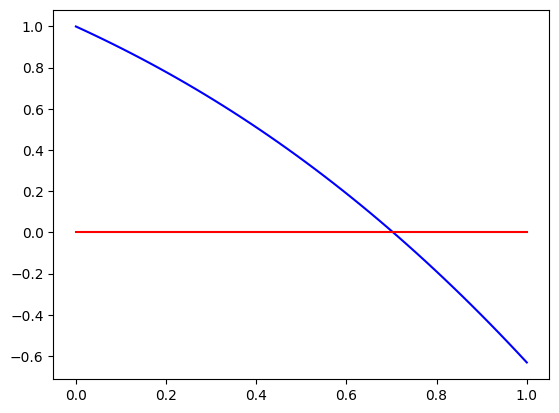
\includegraphics[width=0.6\linewidth]{Clase14_Practica6/bisect_c14p6.png}
\end{figure}

\begin{verbatim}
    def Biseccion(f, a, b, tol):
        cont = 0
        
        while (np.abs(b - a) >= tol):
            if (f(a) * f(b) > 0):
                return ('No hay raices')
            elif (f(a) * f(b) == 0):
                return ('a o b es raiz')
            else:
                c = (a + b) / 2
                cont = cont + 1
                
                print('Pasos = ', cont, 'a = ', a, 'b = ', b, 'c = ', c)
                
                if (f(c) == 0):
                    return ('c es raiz')
                else:
                    if (f(a) * f(c) < 0):
                        b = c
                    else:
                        a = c
                    
        return (a, b, c)
    
    a = 0
    b = 1
    tol = 1 * 10**(-5)
    
    a, b, c = Biseccion(f, a, b, tol)
    
    # Pasos= 1 a= 0 b= 1 c= 0.5
    # Pasos= 2 a= 0.5 b= 1 c= 0.75
    # Pasos= 3 a= 0.5 b= 0.75 c= 0.625
    # Pasos= 4 a= 0.625 b= 0.75 c= 0.6875
    # Pasos= 5 a= 0.6875 b= 0.75 c= 0.71875
    # Pasos= 6 a= 0.6875 b= 0.71875 c= 0.703125
    # Pasos= 7 a= 0.703125 b= 0.71875 c= 0.7109375
    # Pasos= 8 a= 0.703125 b= 0.7109375 c= 0.70703125
    # Pasos= 9 a= 0.703125 b= 0.70703125 c= 0.705078125
    # Pasos= 10 a= 0.703125 b= 0.705078125 c= 0.7041015625
    # Pasos= 11 a= 0.703125 b= 0.7041015625 c= 0.70361328125
    # Pasos= 12 a= 0.703125 b= 0.70361328125 c= 0.703369140625
    # Pasos= 13 a= 0.703369140625 b= 0.70361328125 c= 0.7034912109375
    # Pasos= 14 a= 0.703369140625 b= 0.7034912109375 c= 0.70343017578125
    # Pasos= 15 a= 0.70343017578125 b= 0.7034912109375 c= 0.703460693359375
    # Pasos= 16 a= 0.703460693359375 b= 0.7034912109375 c= 0.7034759521484375
    # Pasos= 17 a= 0.703460693359375 b= 0.7034759521484375 c= 0.7034683227539062	
\end{verbatim}

\subsection{M\'etodo Regula Falsi}

En vez de tomar el punto medio de $[a, b]$, tomamos la ra\'iz de la recta secante que pasa por $(a, f(a))$ y $(b, f(b))$:\\

$$\frac{f(b) - f(a)}{b - a}(x - a) + f(a) = 0 \Rightarrow x = \frac{af(b) - bf(a)}{f(b) - f(a)}$$

\begin{itemize}
    \item Tomo $[a, b]$ un intervalo tal que $f(a)f(b) < 0$

    \item Calculo $c = \frac{af(b) - bf(a)}{f(b) - f(a)}$:\\

    Si $f(c) = 0$, ya est\'a.\\
    
    Si $f(a)f(c) > 0 \Rightarrow$ $f(a)$ y $f(c)$ tienen el mismo signo y la ra\'iz est\'a en $[c, b]$.\\
    
    Si $f(a)f(c) < 0 \Rightarrow$ $f(a)$ y $f(c)$ tienen distinto signo y la ra\'iz est\'a en $[a, c]$.\\

    \item Repito el proceso en el nuevo intervalo
\end{itemize}

\subsection{M\'etodo de Newton-Raphson}

Si $f$ es derivable, en vez de tomar la ra\'iz de la recta secante, tomamos la ra\'iz de la recta tangente. ¿C\'omo?\\

$$x_{0} \rightarrow f'(x_{0})(x - x_{0}) + f(x_{0}) = 0 \rightarrow x_{1} = x_{0} - \frac{f(x_{0})}{f'(x_{0})}$$

si $f'(x_{0}) \neq 0$. Siguiendo con la iteraci\'on

$$f'(x_{1})(x - x_{1}) + f(x_{1}) = 0\ ...$$

\begin{itemize}
    \item Tomo $x_{0} \in [a, b]$

    \item Para $n = 0, 1, 2, ...$, $x_{n + 1} = x_{n} - \frac{f(x_{n})}{f'(x_{n})}$
\end{itemize}

Este m\'etodo no siempre converge.\\

\underline{Error en el m\'etodo de Newton-Raphson}\\

Llamemos $e_{n} = x_{n} - r$. Por Taylor:

$$0 = f(r) = f(x_{n}) + f'(x_{n})(r - x_{n}) + \frac{f''(\theta_{n})}{2}(r - x_{n})^{2}$$

con $\theta$ entre $r$ y $x_{n}$.\\

Despejando, $f'(x_{n})(x_{n} - r) - f(x_{n}) = \frac{f''(\theta_{n})}{2}e_{n}^{2}$. Entonces, diviendo por $f'(x_{n})$:\\

$$x_{n} - r - \frac{f(x_{n})}{f'(x_{n})} = \frac{f''(\theta_{n})}{2f'(x_{n})}e_{n}^{2} \Rightarrow x_{n + 1} - r = \frac{f''(\theta_{n})}{2f'(x_{n})}e_{n}^{2}$$\\

Nos queda:

$$e_{n + 1} = \frac{f''(\theta_{n})}{2f'(x_{n})}e_{n}^{2}$$\\

Debemos pedir $f$ con derivadas hasta orden 2 continuas y $f' \neq 0$. Notemos que, si el m\'etodo converge,\\

$$\frac{e_{n + 1}}{e_{n}} = \frac{f''(\theta_{n})}{2f'(x_{n})} \rightarrow \frac{f''(r)}{2f'(r)} < \infty$$\\

lo hace con orden (al menos) 2.\\

Casos de convergencia para todo $x_{0}$ inicial:

\begin{itemize}
    \item $f' > 0, f'' > 0$ en todo $\mathbb{R}$
    \item $f' > 0, f'' < 0$ en todo $\mathbb{R}$
    \item $f' < 0, f'' > 0$ en todo $\mathbb{R}$
    \item $f' < 0, f'' < 0$ en todo $\mathbb{R}$
\end{itemize}

\subsubsection{Convergencia local del m\'etodo de Newton-Raphson}

Si $f$ tiene dos derivadas continuas en $[a, b], f(r) = 0, f'(r) \neq 0, r \in (a, b)$. Entonces, existe $[c, d] \subseteq [a, b]$ con $r \in [c, d]$ tal que si $x_{0} \in [c, d]$, entonces el m\'etodo converge a $r$. ¿C\'omo encuentro $[c, d]$?\\

Consideramos un intervalo $I \subseteq [a, b]$ tal que $r \in I$ (lo puedo verificar por Bolzano) y adem\'as

$$max_{z \in I} |f''(z)| \leq M$$
$$min_{z \in I} |f'(z)| \geq m$$\\

Sea $L$ tal que $\frac{M}{2m}L < 1$ (o sea $L < \frac{2m}{M}$) y consideramos $[c, d]$ tal que

$$r \in [c, d]$$
$$d - c \leq L$$
$$[c - L, d + L] \subseteq I$$\\

Veamos: si $x_{0} \in [c, d] \Rightarrow |e_{0}| \leq L$ y como $|f''(z)| \leq M, |f'(z)| \geq m\ \forall z \in [c, d]$,

$$|e_{1}| = \frac{f''(\theta_{n})}{2f'(x_{0})}|e_{0}|^{2} \leq \frac{M}{2m}|e_{0}||e_{0}| \leq \frac{M}{2m}L|e_{0}| = \lambda|e_{0}|$$\\

Como $\lambda < 1$, tenemos $|e_{1}| < |e_{0}| < L$ y $x_{1} \in I$, $\theta_{1} \in I$

$$|e_{2}| = \frac{f''(\theta_{n})}{2f'(x_{1})}|e_{1}|^{2} \leq \frac{M}{2m}|e_{1}||e_{1}| \leq \frac{M}{2m}L|e_{1}| = \lambda|e_{1}| \leq \lambda^{2}|e_{0}$$
$$ ... $$
$$ |e_{n}| \leq \lambda^{n}|e_{0}|$$\\

Como $\lambda < 1$, tenemos $\lim\limits_{n \to \infty}{|e_{n}|} = 0$.\\

\textit{Python}: M\'etodo de Newton - Raphson\\

Utilizar el m\'etodo de Newton - Raphson con $x_{0} = 0$ para aproximar la soluci\'on de la ecuaci\'on $e^{-x} = x^{2}$ en el intervalo $[0, 1]$. Analizar la convergencia.\\

\begin{verbatim}
	import numpy as np
	import matplotlib.pyplot as plt
	
	def f(x):
	    return (np.exp(-x) - x**2)
	    
	x = np.linspace(0, 1, 50)
	
	plt.plot(x, f(x), 'b', x, np.zeros(len(x)), 'r')		
\end{verbatim}

\begin{figure}[H]
  \centering
  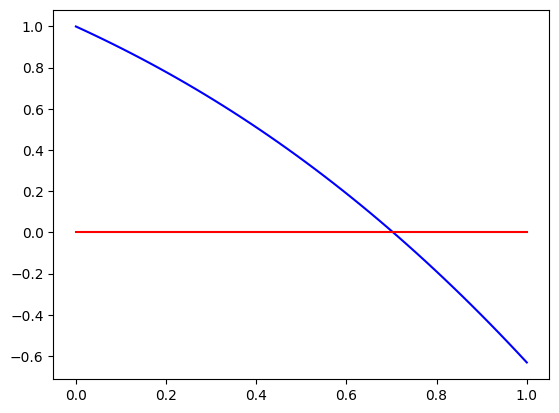
\includegraphics[width=0.6\linewidth]{Clase14_Practica6/bisect_c14p6.png}
\end{figure}

\begin{verbatim}
    def Derf(x):
        return (-1 * np.exp(-x) - 2 * x)
        
    def Newton(f, Derf, x0, MaxIter, tol):
        x1 = x0 - (f(x0) / Derf(x0))
        
        i = 1
        
        while ((i < MaxIter) and (np.abs(x0 - x1) > tol)):
            i = i + 1
            x0 = x1
            x1 = x0 - (f(x0) / Derf(x0))
            
            print('i = ', i, 'x1 = ', x1)
            
        return (i, x1)
        
    x0 = 0
    MaxIter = 100
    tol = 1 * 10**(-5)
    
    i, x1 = Newton(f, Derf, x0, MaxIter, tol)
    
    # i = 2 x1 = 0.7330436052454454
    # i = 3 x1 = 0.703807786324133
    # i = 4 x1 = 0.7034674683317975
    # i = 5 x1 = 0.7034674224983924
    
    # Probamos con otra semilla
    x0 = -500
    MaxIter = 1000
    
    i, x1 = Newton(f, Derf, x0, MaxIter, tol)

    # i = 2 x1 = -498.0
    # i = 3 x1 = -497.0
    # i = 4 x1 = -496.0
    # ...
    # i = 505 x1 = 0.703467440228491
    # i = 506 x1 = 0.7034674224983918
\end{verbatim}
\newpage
\section{Clase 15 - Pr\'actica 6 (Resoluci\'on num\'erica de ecuaciones no lineales)}

\subsection{M\'etodo de la secante}

Comenzamos con dos valores $x_{0}$ y $x_{1}$ cercanos a la ra\'iz (podr\'ian estar los dos a la izquierda o a la derecha de la ra\'iz) y construimos $x_{2}$ como la ra\'iz de la recta secante que pasa por $(x_{0}, f(x_{0}))$ y $(x_{1}, f(x_{1}))$.

$$\frac{f(x_{1}) - f(x_{0})}{x_{1} - x_{0}}(x - x_{1}) + f(x_{1}) = 0$$

$$\Rightarrow x_{2} = x_{1} - \frac{f(x_{1})}{\frac{f(x_{1}) - f(x_{0})}{x_{1} - x_{0}}}$$

\begin{itemize}
    \item Tomo $x_{0}$ y $x_{1}$ dos valores aproximados de $r$, la ra\'iz de $f$.\\

    \item Para $n = 1, 2, ..., x_{n + 1} = x_{n} - \frac{f(x_{n})}{\frac{f(x_{n}) - f(x_{n - 1})}{x_{n} - x_{n - 1}}}$
\end{itemize}

\underline{Error en el m\'etodo de la secante}

$$e_{n + 1} = \frac{f''(\eta_{n})}{2f'(\theta_{n})} = e_{n}e_{n - 1}$$

con $\eta_{n}, \theta_{n} \in [a, b]$.\\

\textit{Idea sobre el orden de convergencia}: si $p$ es tal que $e_{n + 1} \sim C|e_{n}|^{p} \Rightarrow |e_{n + 1}| \sim C|e_{n}|^{p} \sim C(C|e_{n - 1}|^{p})^{p} \sim C^{p + 1}|e_{n - 1}|^{p^{2}}$.\\

Por la f\'ormula del error sabemos que $|e_{n + 1}| \sim K|e_{n}||e_{n - 1}|$ y reemplazando en lo anterior nos queda

$$K|e_{n}||e_{n - 1}| \sim C^{p + 1}|e_{n - 1}|^{p^{2}}$$

y de aqu\'i

$$KC|e_{n - 1}|^{p}|e_{n - 1}| \sim C^{p + 1}|e_{n - 1}|^{p^{2}}$$

Entonces

$$\frac{K}{C^{p}}|e_{n - 1}|^{p + 1} \sim |e_{n - 1}|^{p^{2}} \Rightarrow |e_{n - 1}|^{p^{2} - p - 1} \sim cte$$\\

Deber\'ia ser entonces $p^{2} - p - 1 = 0$ y la soluci\'on positiva de esta ecuaci\'on en $p = \frac{1 + \sqrt{5}}{2}$ (el n\'umero de oro).

\subsection{M\'etodo de punto fijo}

La idea ahora es reformular el problema de "hallar $x$ tal que $f(x) = 0$" en otro equivalente de la forma "hallar $x$ tal que $x = g(x)$".\\

\textit{Ejemplo}: $4x^{3} - 2x - 5 = 0$ es equivalente a

\begin{itemize}
    \item $x = \frac{4x^{3} - 5}{2}$, donde $g_{1}(x) = \frac{4x^{3} - 5}{2}$
    
    \item $x = \sqrt[3]{\frac{2x + 5}{4}}$, donde $g_{2}(x) = \sqrt[3]{\frac{2x + 5}{4}}$
    
    \item $x = \frac{2x + 5}{4x^{2}}$, donde $g_{3}(x) = \frac{2x + 5}{4x^{2}}$
\end{itemize}

\textit{Cuidado}: No cualquier reformulaci\'on va a servir.\\

\underline{Definici\'on}: Decimos que $r$ es punto fijo de $g$ si $g(r) = r$.\\

\begin{itemize}
    \item Tomo $x_{0}$ una aproximaci\'on de $r$.

    \item Para $n = 0, 1, 2, ...$, $x_{n + 1} = g(x_{n})$ .
\end{itemize}

\textit{Observaci\'on}: el m\'etodo de Newton-Raphson se puede ver como un m\'etodo de punto fijo para el problema $x = g(x)$ con $g(x) = x - \frac{f(x)}{f'(x)}$\\

¿Bajo que condiciones converge el m\'etodo de punto fijo?\\

\underline{Definici\'on}: Decimos que una funci\'on $g: [a, b] \rightarrow \mathbb{R}$ es contractiva (o es una contracci\'on) en el intervalo $[a, b]$ si existe una constante $L, 0 \leq L < 1$ tal que $|g(x) - g(y)| \leq L|x - y|$ para cualquiera $x, y \in [a, b]$\\

\underline{Teorema}: Sea $g: [a, b] \rightarrow \mathbb{R}$ continua tal que

\begin{itemize}
    \item $g([a, b]) \subseteq [a, b]$
    
    \item $g$ es contractiva en $[a, b]$ con cte $0 \leq L < 1$, entonces el m\'etodo de punto fijo $x_{n + 1} = g(x_{n})$ converge al (\'unico) punto fijo $r \in [a, b]$. Es decir, $\lim_{n \to \infty} x_{n} = r$ con $g(r) = r$.
\end{itemize}

¿C\'omo verifico que $g$ es contractiva?\\

Por el Teorema de Valor Medio de Lagrange, si $g$ es derivable podemos escribir para cualesquiera $x, y \in [a, b]$:\\

$$|g(x) - g(y)| = |g'(\theta)||x - y| \leq \max_{\theta \in [a, b]} |g'(\theta)||x - y|$$

Luego, para ver que $g$ es contractiva, basta con encontrar $0 \leq L < 1$ tal que $\max_{\theta \in [a, b]} |g'(\theta)| \leq L$.\\

¿Por qu\'e converge el m\'etodo?\\

Al pedir $g([a, b]) \subseteq [a, b]$ garantizamos que si $x_{0} \in [a, b]$ entonces toda la sucesi\'on quedar\'a en $[a, b]$:

$$x_{0} \in [a, b] \Rightarrow x_{1} = g(x_{0}) \in [a, b] \Rightarrow x_{2} = g(x_{1}) \in [a, b]\ ...$$

Como $g$ es contractiva,

$$|e_{n + 1}| = |x_{n + 1} - r| = |g(x_{n}) - g(r)| \leq L|x_{n} - r| = L|e_{n}|$$

y con este razonamiento se obtiene

$$|e_{n + 1}| \leq L|e_{n}| \leq L^{2}|e_{n - 1}| \leq ... \leq L^{n + 1}|e_{0}| \rightarrow_{n \to +\infty} 0$$

pues $L < 1$.\\

\underline{Error de punto fijo}

\begin{itemize}
    \item $|x_{n} - r| \leq L^{n}|x_{0} - r|$

    \item $|x_{n} - r| \leq \frac{L^{n}}{1 - L}|x_{1} - x_{0}|$

    \item $|x_{n} - r| \leq \frac{L}{1 - L}|x_{n} - x_{n - 1}|$
\end{itemize}
\newpage
\section{Clase 16 - Pr\'actica 6 (Resoluci\'on num\'erica de ecuaciones no lineales) y Pr\'actica 7 (Interpolaci\'on)}

\subsection{Orden de convergencia}

Sea $\{a_{n}\}_{n \in \mathbb{N}}$ una sucesi\'on de n\'umeros reales, $a_{n} \rightarrow_{n \to \infty} l, l \in \mathbb{R}$. Decimos que $a_{n}$ converge a $l$ con orden al menos $p$ si existen $C > 0, n_{0} \in \mathbb{N}$ tales que $\frac{|a_{n + 1} - l|}{|a_{n} - l|} \leq C\ \forall n \geq n_{0}$.\\

Decimos que $a_{n}$ converge a $l$ con orden exactamente $p$ si converge con orden al menos $p$ y $\forall \epsilon > 0$ $\frac{|a_{n + 1} - l|}{|a_{n} - l|^{p - \epsilon}} \rightarrow_{n \to +\infty} 0$.\\

\underline{Ra\'ices m\'ultiples}\\

Sea $r$ tal que $f(r) = 0, ..., f^{(p - 1)}(r) = 0, f \in C^{p}$. Adem\'as, $f(x) = (x - r)^{p}g(x), g(r) \neq 0, g \in C^{1}$\\

\begin{itemize}
    \item Para Newton-Raphson:

    $$x_{n + 1} = x_{n} - \frac{(x_{n} - r)^{p}g(x_{n})}{p(x_{n} - r)^{p - 1}g(x_{n}) + (x_{n} - r)^{p}g'(x_{n})}$$

    $$e_{n + 1} = e_{n} - \frac{e_{n}^{p}g(x_{n})}{pe_{n}^{p - 1}g(x_{n}) + e_{n}^{p}g'(x_{n})} = e_{n} - \frac{e_{n}g(x_{n})}{pg(x_{n}) + e_{n}g'(x_{n})}$$

    $$\Rightarrow e_{n + 1} = e_{n}\frac{(p - 1)g(x_{n})}{pg(x_{n}) + e_{n}g'(x_{n})} + e_{n}^{2}\frac{g'(x_{n})}{pg(x_{n}) + e_{n}g'(x_{n})}$$

    Si $x_{n} \rightarrow r$ y $p \neq 1$,

    $$\frac{(p - 1)g(x_{n})}{pg(x_{n}) + e_{n}g'(x_{n})} \rightarrow \frac{(p - 1)g(r)}{pg(r)} = \frac{p - 1}{p} \neq 0$$

    y la convergencia es lineal.\\

    \item Para punto fijo:\\

    Si $g \in C^{1}$ y $x_{n + 1} = g(x_{n}) \rightarrow r$,

    $$e_{n + 1} = x_{n + 1} - r = g(x_{n}) - g(r) = g'(\zeta_{n})(x_{n} - r) = g'(\zeta_{n})e_{n}$$

    Si $e_{n} \neq 0, \frac{e_{n + 1}}{e_{n}} = g'(\zeta_{n})) \rightarrow g'(r)$. Si $g'(r) \neq 0$, la convergencia es lineal. Si $g \in C^{p}, g^{(k)} = 0$ para $1 \leq k \leq p, g^{(p)} \neq 0$,

    $$e_{n + 1} = x_{n + 1} - r = g(x_{n}) - g(r) = g'(r)(x_{n} - r) + \frac{g''(r)}{2}(x_{n} - r)^{2} + ... + \frac{g^{(p)}(\zeta_{n})}{p!}(x_{n} - r)^{p}$$

    $$\Rightarrow e_{n + 1} = \frac{g^{(p)}(\zeta_{n})}{p!}e_{n}^{p} \Rightarrow \frac{e_{n + 1}}{e_{n}} \rightarrow \frac{g^{(p)}(r)}{p!} \neq 0$$

    y el m\'etodo tiene orden $p$.
\end{itemize}

\subsection{Sistemas de ecuaciones no lineales}

$$
    \begin{cases}
        f_{1}(x, y) = 0\\
        f_{2}(x, y) = 0
    \end{cases}
$$\\

Llamamos $F(x, y) = (f_{1}(x, y), f_{2}(x, y)),\ F: \mathbb{R}^{2} \rightarrow \mathbb{R}^{2}$. Buscamos $\Vec{r} = (r_{1}, r_{2})$ tal que $F(\Vec{r}) = (0, 0)$.\\

\underline{Newton-Raphson}\\

Recordemos la ecuaci\'on del plano tangente en $(x_{0}, y_{0}, f(x_{0}, y_{0}))$:

$$z - f(x_{0}, y_{0}) = \frac{\partial f}{\partial x}(x_{0}, y_{0})(x - x_{0}) + \frac{\partial f}{\partial y}(x_{0}, y_{0})(y - y_{0})$$\\

Propongo $(x_{1}, y_{1})$ tal que:

$$ 0 = \frac{\partial f_{i}}{\partial x}(x_{0}, y_{0})(x_{1} - x_{0}) + \frac{\partial f_{i}}{\partial y}(x_{0}, y_{0})(y_{1} - y_{0}) + f_{i}(x_{0}, y_{0}),\ i = 1, 2$$\\

Reordeno:

$$ -\frac{\partial f_{i}}{\partial x}(x_{0}, y_{0})x_{1} - \frac{\partial f_{i}}{\partial y}(x_{0}, y_{0})y_{1} = -\frac{\partial f_{i}}{\partial x}(x_{0}, y_{0})x_{0} - \frac{\partial f_{i}}{\partial y}(x_{0}, y_{0})y_{0} + f_{i}(x_{0}, y_{0}),\ i = 1, 2$$\\

En forma matricial:

$$    -
    \begin{pmatrix}
        \frac{\partial f_{1}}{\partial x}(x_{0}, y_{0}) & \frac{\partial f_{1}}{\partial y}(x_{0}, y_{0})\\
        \frac{\partial f_{2}}{\partial x}(x_{0}, y_{0}) & \frac{\partial f_{2}}{\partial y}(x_{0}, y_{0})
    \end{pmatrix}
    \begin{pmatrix}
        x_{1}\\
        y_{1}
    \end{pmatrix}
    = -
    \begin{pmatrix}
        \frac{\partial f_{1}}{\partial x}(x_{0}, y_{0}) & \frac{\partial f_{1}}{\partial y}(x_{0}, y_{0})\\
        \frac{\partial f_{2}}{\partial x}(x_{0}, y_{0}) & \frac{\partial f_{2}}{\partial y}(x_{0}, y_{0})
    \end{pmatrix}
    \begin{pmatrix}
        x_{0}\\
        y_{0}
    \end{pmatrix}
    +
    \begin{pmatrix}
        f_{1}(x_{0}, y_{0})\\
        f_{2}(x_{0}, y_{0})
    \end{pmatrix}
$$\\

Si

$$J_{n} = Jac\ F(x_{n}, y_{n}) = \begin{pmatrix}
        \frac{\partial f_{1}}{\partial x}(x_{n}, y_{n}) & \frac{\partial f_{1}}{\partial y}(x_{n}, y_{n})\\
        \frac{\partial f_{2}}{\partial x}(x_{n}, y_{n}) & \frac{\partial f_{2}}{\partial y}(x_{n}, y_{n})
    \end{pmatrix}$$

y $J_{n}^{-1}$ su inversa, el m\'etodo es:

\begin{itemize}
    \item Tomo $x_{0} \in \mathbb{R}^{2}$ que aproxima a $\Vec{r}$

    \item Para $n = 0, 1, 2, ...$, $\Vec{x}_{n + 1} = \Vec{x}_{n} - J_{n}^{-1}F(\Vec{x}_{n})$\\

    \textit{Observaci\'on}: $J_{n}^{-1}F(\Vec{x}_{n}) = \Vec{v}_{n} \iff J_{n}\Vec{v}_{n} = F(\Vec{x}_{n})$. Es decir, $\Vec{v}_{n}$ es la soluci\'on del sistema lineal $A\Vec{x} = \Vec{b}$, con $A = J_{n}$ y $\Vec{b} = F(\Vec{x}_{n})$.\\
\end{itemize}

\underline{Punto fijo}

$$F(x, y) = (0, 0) \Rightarrow G(x, y) = (x, y)$$

El m\'etodo nos queda:

\begin{itemize}
    \item Tomo $x_{0} \in \mathbb{R}^{2}$ que aproxima a $\Vec{r}$

    \item Para $n = 0, 1, 2, ...$, $\Vec{x}_{n + 1} = G(\Vec{x}_{n})$\\
\end{itemize}

\textit{Ejemplo}: Aproximar por el m\'etodo de Newton las $x$ del sistema no lineal

$$
    \begin{cases}
        x^{2} + y^{2} = 10\\
        x^{2} - y^{2} = 1
    \end{cases}
$$\\

Tenemos $f_{1}(x, y ) = x^{2} + y^{2} - 10$ y $f_{2}(x, y) = x^{2} - y^{2} - 1$. Entonces

$$Jac\ F(x, y) = \begin{pmatrix}
        2x & 2y\\
        2x & -2y
    \end{pmatrix}$$\\

\underline{\textbf{Interpolaci\'on}}\\

Partimos de una tabla de datos

\begin{table}[h]
    \centering
    \begin{tabular}{|c|c|c|c|c|c|}
        \hline
        $x$ & $x_{0}$ & $x_{1}$ & $x_{2}$ & $...$ & $x_{n}$\\ \hline
        $y$ & $y_{0}$ & $y_{1}$ & $y_{2}$ & $...$ & $y_{n}$\\ \hline
    \end{tabular}
\end{table}

con $x_{0}, x_{1}, \cdots , x_{n}$ distintos. Buscamos un polinomio de grado $\leq n$ que pase por esos puntos.\\

\underline{Teorema}: Dados $n + 1$ valores distintos $x_{0}, x_{1}, \cdots , x_{n}$ y $n + 1$ valores cualesquiera $y_{0}, y_{1}, \cdots , y_{n}$, existe un polinomio $P_{n}$ de grado $\leq n$ que satisface $P_{n}(x_{i}) = y_{i}, \ i = 0, \cdots , n$.\\

Si $y_{i} = f(x_{j})$ para cierta funci\'on $f$, decimos que $P_{n}$ interpola a $f$ en $x_{0}, ... , x_{n}$.\\

Vamos a ver tres maneras de armar $P_{n}$: coeficientes indeterminados, forma de Lagrange y forma de Newton (tabla de diferencias finitas).\\

\subsection{Coeficientes indeterminados}

$$P_{n}(x) = a_{0} + a_{1}x + a_{2}x^{2} + ... + a_{n}x^{n}$$

y resuelvo un sistema lineal para hallar $a_{0}, ... ,a_{n}$.\\

$$P_{n}(x_{0}) = a_{0} + a_{1}x_{0} + a_{2}x_{0}^{2} + ... + a_{n}x_{0}^{n} = y_{0}$$
$$ \vdots $$
$$P_{n}(x_{n}) = a_{0} + a_{1}x_{n} + a_{2}x_{n}^{2} + ... + a_{n}x_{n}^{n} = y_{n}$$\\

En forma matricial (matriz de Vandermonde):

$$
    \begin{pmatrix}
        1 & x_{0} & x_{0}^{2} & \cdots & x_{0}^{n}\\
        \vdots & \vdots & \vdots & \cdots & \vdots\\
        \vdots & \vdots & \vdots & \cdots & \vdots\\
        1 & x_{n} & x_{n}^{2} & \cdots & x_{n}^{n}\\
    \end{pmatrix}
    \begin{pmatrix}
        a_{0}\\
        a_{1}\\
        \vdots\\
        a_{n}\\
    \end{pmatrix}
    =
    \begin{pmatrix}
        y_{0}\\
        y_{1}\\
        \vdots\\
        y_{n}\\
    \end{pmatrix}
$$\\

\textit{Ejemplo}:

\begin{table}[h]
    \centering
    \begin{tabular}{|c|c|c|c|}
        \hline
        $x$ & -1 & 0 & 1\\ \hline
        $y$ & 12 & 5 & 4\\ \hline
    \end{tabular}
\end{table}

Tenemos 3 puntos, luego $n = 2 \rightarrow P_{2}(x) = a_{0} + a_{1}x + a_{2}x^{2}$, armamos la matriz de Vandermonde y resolvemos:

$$
    \begin{pmatrix}
        1 & -1 & 2\\
        1 & 0 & 0\\
        1 & 1 & 1\\
    \end{pmatrix}
    \begin{pmatrix}
        a_{0}\\
        a_{1}\\
        a_{2}\\
    \end{pmatrix}
    =
    \begin{pmatrix}
        12\\
        5\\
        4\\
    \end{pmatrix}
$$\\

$$ \Rightarrow P_{2}(x) = 5 - 4x + 3x^{2}$$

\subsection{Forma de Lagrange}

$$P_{n}(x) = y_{0}l_{0}(x) + y_{1}l_{1}(x) + y_{2}l_{2}(x) + \cdots + y_{n}l_{n}(x)$$\\

con $l_{0}, l_{1}, \cdots, l_{n}$ polinomios tales que $l_{i}(x_{j}) = \delta_{ij}$.\\

Expl\'icitamente:

$$l_{j}(x) = \frac{(x - x_{0})(x - x_{1})(x - x_{j - 1})(x - x_{j + 1})\cdots(x - x_{n})}{(x_{j} - x_{0})(x_{j} - x_{1})(x_{j} - x_{j - 1})(x_{j} - x_{j + 1})\cdots(x_{j} - x_{n})}$$\\

con $\{l_{0}, \cdots, l_{n}\}$ base de Lagrange.\\

\textit{Ejemplo anterior}:

$$P_{2}(x) = y_{0}l_{0}(x) + y_{1}l_{1}(x) + y_{2}l_{2}(x) = 12l_{0}(x) + 5l_{1}(x) + 4l_{2}(x)$$

$$l_{0}(x) = \frac{(x - 0)(x - 1)}{(-1 + 0)(-1 - 1)} = \frac{1}{2}x(x - 1)$$

$$l_{1}(x) = \frac{(x + 1)(x - 1)}{(0 + 1)(0 - 1)} = -(x + 1)(x - 1)$$

$$l_{2}(x) = \frac{(x + 1)(x - 0)}{(1 + 1)(1 - 0} = \frac{1}{2}(x + 1)x$$

$$\Rightarrow P_{2}(x) = 12\frac{1}{2}x(x - 1) - 5(x + 1)(x - 1) + 4\frac{1}{2}(x + 1)x = 3x^{2} - 4x + 5$$

\subsection{Forma de Newton - Tabla de diferencias divididas}

\begin{table}[h]
    \centering
    \begin{tabular}{c|ccc}
        $x_{i}$ & $f[\cdot]$ & $f[\cdot, \cdot]$ & $f[\cdot, \cdot, \cdot]$\\ \hline
        $x_{0}$ & $f(x_{0})$ &  & \\
        &&&\\
        $x_{1}$ & $f(x_{1})$ & $f[x_{0}, x_{1}] = \frac{f(x_{1}) - f(x_{0})}{x_{1} - x_{0}}$ & \\
        &&&\\
        $x_{2}$ & $f(x_{2})$ & $f[x_{1}, x_{2}] = \frac{f(x_{2}) - f(x_{1})}{x_{2} - x_{1}}$ & $f[x_{0}, x_{1}, x_{2}] = \frac{f[x_{1}, x_{2}] - f[x_{0}, x_{1}]}{x_{2} - x_{0}}$\\
    \end{tabular}
\end{table}

$$P_{n}(x) = f[x_{0}] + f[x_{0}, x_{1}](x - x_{0}) + f[x_{0}, x_{1}, x_{2}](x - x_{0})(x - x_{1}) + \cdots + f[x_{0}, \cdots, x_{n}](x - x_{0})...(x - x_{n - 1})$$\\

\underline{Definici\'on}: Diferencias divididas

\begin{itemize}
    \item $f[x_{i}] = f(x_{i})$, de orden 0.
    \item $f[x_{i}, x_{i + 1}, \cdots, x_{i + m}] = \frac{f[x_{i + 1}, \cdots, x_{i + m}] - f[x_{i}, \cdots, x_{i + m - 1}]}{x_{i + m} - x_{i}}$, de orden $m$.\\
\end{itemize}

\newpage
\textit{Ejemplo anterior}:

\begin{table}[h]
    \centering
    \begin{tabular}{c|ccc}
        $x_{i} $ & $f[\cdot]$ & $f[\cdot, \cdot]$ & $f[\cdot, \cdot, \cdot]$\\ \hline
        $x_{0} = -1$ & 12 &  & \\
        &&&\\
        $x_{1} = 0$ & 5 & $\frac{5 - 12}{0 - (-1)} = -7$ & \\
        &&&\\
        $x_{2} = 1$ & 4 & $\frac{4 - 5}{1 - 0} = -1$ & $\frac{-1 - (-7)}{1 - (-1)} = 3$\\
    \end{tabular}
\end{table}

$$\Rightarrow P_{2}(x) = 12 - 7(x - (-1)) + 3(x - 0)(x - (-1)) = 3x^{2} - 4x + 5$$\\

\textit{Observaci\'on}:

\begin{itemize}
    \item Si $y_{i} = f(x_{i})$ y $f$ es un polinomio de grado $\leq n \Rightarrow P_{n} = f$.
    \item Hay infinitos polinomios de grado $\geq n + 1$ que interpolan en $n$ puntos. Por ejemplo: $P_{n + 1}(x) = P_{n}(x) + \alpha(x - x_{0})(x - x_{1})...(x - x_{n}),\ \alpha \in \mathbb{R}$\\
\end{itemize}

\underline{Error de interpolaci\'on}: $f:[a, b] \rightarrow \mathbb{R},\ x_{0}, \cdots, x_{n} \in [a, b]$ todos distintos, $x \in [a, b]$:

$$f(x) - P_{n}(x) = \frac{f^{(n + 1)}(\theta)}{(n + 1)!}\prod_{j = 0}^{n} (x - x_{j}),\ \theta \in [a, b]$$
\newpage
\section{Clase 17 - Pr\'actica 7 (Interpolaci\'on)}

\subsection{Forma de Newton - Tabla de diferencias divididas}

Por qu\'e interpola?

\begin{itemize}
	\item Si $n = 0$: $P_{0} = f[x_{0}] = f(x_{0})$
	\item Si $n = 1$: $P_{1} = f[x_{0}] + f[x_{0}, x_{1}](x - x_{0}) = f(x_{0}) + \frac{f(x_{1}) - f(x_{0}}{x_{1} - x_{0}}(x - x_{0})$, (la recta secante).
	\item Consideremos $x_{0}, x_{1}, \cdots, x_{n + 1}$ $n + 2$ puntos distintos. Supongamos que $P_{n} = f[x_{0}] + f[x_{0}, x_{1}](x - x_{0}) + \cdots + f[x_{0}, \cdots, x_{n}](x - x_{0})...(x - x_{n})$ verifica $P_{n}(x_{i}) = y_{i}$ para $i = 0, \cdots, n$ y que $\tilde{P}_{n} = f[x_{1}] + f[x_{1}, x_{2}](x - x_{1}) + \cdots + f[x_{1}, \cdots, x_{n + 1}](x - x_{1})...(x - x_{n})$ verifica $\tilde{P}_{n}(x_{i}) = y_{i}$ para $i = 1, \cdots, n + 1$.\\
	
	Sea $Q$ el polinomio de grado $\leq n + 1$ que interpola a $f$ en $x_{0}, \cdots, x_{n + 1}$, veamos que $Q = f[x_{0}] + \cdots + f[x_{0}, \cdots, x_{n + 1}](x - x_{0})...(x - x_{n})$.
\end{itemize}

Todo polinomio en $\mathcal{P}_{n + 1}$ se puede escribir en la base $\{1, (x - x_{0}), (x - x_{0})(x - x_{1}), \cdots, (x - x_{0})(x - x_{1})...(x - x_{n})\}$

$$Q(x) = a_{0} + a_{1}(x - x_{0}) + \cdots + a_{n + 1}(x - x_{0})(x - x_{1})...(x - x_{n}) = P(x) + a_{n + 1}(x - x_{0})(x - x_{1})...(x - x_{n})$$

Como $Q(x_{i}) = P(x_{i})$ para $i = 0, \cdots, n$ y $P$ tiene grado $n$, necesariamente $P = P_{n}$. Consideremos el polinomio

$$\tilde{Q}({x}) = \frac{(x - x_{0})\tilde{P}_{n} - (x - x_{n + 1})P_{n}}{x_{n + 1} - x_{0}}$$

El grado de $\tilde{Q}$ es $\leq n + 1$ y vale que

$$\tilde{Q}({x_{i}}) = \frac{(x_{i} - x_{0})\tilde{P}_{n}(x_{i}) - (x_{i} - x_{n + 1})P_{n}(x_{i})}{x_{n + 1} - x_{0}} = f(x_{i})\frac{(x_{i} - x_{0}) - (x_{i} - x_{n + 1})}{x_{n + 1} - x_{0}} = f(x_{i})$$

para $i = 1, \cdots, n$.\\

$$\tilde{Q}({x_{0}}) = \frac{-(x_{0} - x_{n + 1})f(x_{0})}{x_{n + 1} - x_{0}} = f(x_{0})$$
$$\vdots$$
$$\tilde{Q}({x_{n + 1}}) = \frac{(x_{n + 1} - x_{0})f(x_{n + 1})}{x_{n + 1} - x_{0}} = f(x_{n + 1})$$

Por lo tanto, $\tilde{Q} = Q$. Si $a_{n + 1} \neq 0,\ a_{n + 1} = \text{coef ppal}(\tilde{Q}) = \frac{f[x_{1}, \cdots, x_{n + 1}] - f[x_{0}, \cdots, x_{n}]}{x_{n + 1} - x_{0}} = f[x_{0}, \cdots, x_{n + 1}]$.\\

\underline{Teorema}: Sean $x_{0}, \cdots, x_{n}$ puntos distintos y sea $z_{0}, \cdots, z_{n}$ una permutaci\'on de $x_{0}, \cdots, x_{n}\Rightarrow f[x_{0}, \cdots, x_{n}] = f[z_{0}, \cdots, z_{n}]$.\\

La demostraci\'on se basa en el hecho de que el polinomio de $\mathcal{P}_{n}$ que interpola en $x_{0}, \cdots, x_{n}$ y en $z_{0}, \cdots, z_{n}$ es el mismo y su coeficiente principal es la diferencia dividida correspondiente.\\

\underline{\textit{Error de interpolaci\'on}}:\\

\underline{Teorema}: $f: [a, b] \rightarrow \mathbb{R}, x_{0}, x_{1}, \cdots, x_{n} \in [a, b]$ distintos, $x \in [a, b]$:

$$f(x) - P_{n}(x) = \frac{f^{(n + 1)}(\zeta)}{(n + 1)!}W_{n + 1}(x)$$

con $\zeta \in [a, b],\ W_{n + 1}(x) = \prod\limits_{j = 0}^{n}(x - x_{j})$.\\

\underline{Demostraci\'on}:\\

Si $x = x_{i}$, vale pues $f(x_{i}) = P_{n}(x_{i})$ y $W_{n + 1}(x) = 0$ para $i = 0, \cdots, n$. Si $x \neq x_{i}$ para  $0 \leq i \leq n$, $x \in [a, b]$, definimos

$$F(t) = (f(t) - P_{n}(t))W_{n + 1}(x) - (f(x) - P_{n}(x))W_{n + 1}(t)$$

Como $F(x) = F(x_{0}) = \cdots = F(x_{n}) = 0,\ F$ tiene al menos $n + 2$ ceros distintos en $(a, b)$. Por el teorema de Rolle, $F'$ tiene al menos $n + 1$ ceros distintos en $(a, b)$. Y as\'i, deducimos que $F^{(n + 1)}$ tiene al menos un cero, $\zeta \in (a, b)$:

$$0 = F^{(n + 1)}(\zeta) = f^{(n + 1)}(\zeta)W_{n + 1}(x) - (f(x) - P_{n}(x))(n + 1)!$$

como quer\'iamos probar.\\

\underline{Corolario}: $|f(x) - P_{n}(x)| \leq \max \limits_{a \leq c \leq b} |f^{(n + 1)}(c)|\frac{|W(x)|}{(n + 1)!}$\\

\underline{Definici\'on}: $\|f\|_{\infty, [a, b]} = \max \limits_{a \leq x \leq b} |f(x)|$\\

\underline{Teorema}: $f(x) - P_{n}(x) = f[x_{0}, \cdots, x_{n}, x]W_{n + 1}(x)$\\

\underline{Demostraci\'on}: Sea $P_{n + 1}$ el polinomio de $\mathcal{P}_{n + 1}$ que interpola a $f$ en $x_{0}, \cdots, x_{n}, x$ en $x \neq x_{i}$ para $0 \leq i \leq n \Rightarrow P_{n + 1}(t) = P_{n}(t) + f[x_{0}, \cdots, x_{n}, x]W_{n + 1}(t)$, y como $P_{n + 1}(x) = f(x)$, vale lo que quer\'iamos.\\

\underline{Corolario}: Sea $f \in C^{n + 1}([a, b]),\ x_{0}, \cdots, x_{n}$ puntos distintos en $[a, b] \Rightarrow \exists \ \zeta \in [a, b] \ / \ f[x_{0}, \cdots, x_{n}] = \frac{f^{(n)}(\zeta)}{n!}$\\

\underline{Teorema}: Si $x_{i} = a + hi$ para $i = 0, 1, \cdots, n \ / \ h = \frac{b - a}{n}$. Entonces para todo $x \in [a, b], \ |W_{n + 1}(x)| \leq \frac{1}{4}h^{n + 1}n!$\\

\underline{Demostraci\'on}: Sea $x \in [a, b]$, existe $j \ / \ x_{j} \leq x \leq x_{j + 1}$. Maximizando la cuadr\'atica $(x - x_{j})(x_{j + 1} - x)$ llegamos a que

$$|x - x_{j}||x - x_{j + 1}| \leq \frac{h^{2}}{4}$$

De esta forma,

$$\prod \limits_{i = 0}^{n} |x - x_{i}| \leq \frac{h^{2}}{4} \prod \limits_{i = 0}^{j - 1} |x - x_{i}|\prod \limits_{i = j + 2}^{n} |x - x_{i}| = \frac{h^{2}}{4} \prod \limits_{i = 0}^{j - 1} |x - x_{i}|\prod \limits_{i = j + 2}^{n} |x_{i} - x|$$

Como $x_{j} \leq x \leq x_{j + 1}$, vale adem\'as que

$$\prod \limits_{i = 0}^{n} |x - x_{i}| \leq \frac{h^{2}}{4} \prod \limits_{i = 0}^{j - 1} |x_{j + 1} - x_{i}|\prod \limits_{i = j + 2}^{n} |x_{i} - x_{j}|$$

y como $x_{i} = a + ih$, $x_{j + 1} - x_{i} = (j - i + 1)h$ y $x_{i} - x_{j} = (i - j)h$

$$\prod \limits_{i = 0}^{n} |x - x_{i}| \leq \frac{h^{2}}{4} h^{j} h^{n - (j + 2) + 1} \prod \limits_{i = 0}^{j - 1} (j - i + 1)\prod \limits_{i = j + 2}^{n} (i - j) \leq \frac{1}{4}h^{n + 1}(j + 1)!(n - j)! \leq \frac{1}{4}h^{n + 1}n!$$

Podemos minimizar el error eligiendo convienientemente los valores $x_{0}, \cdots, x_{n}$? C\'omo podemos minimizar $|W(x)|$?\\

\underline{Teorema}: Si $x_{0}, x_{1}, \cdots, x_{n}$ son los ceros de $T_{n + 1}$, el polinomio de Tchebyshev de grado $n + 1 \Rightarrow$

$$\max \limits_{x \in [-1, 1]} \prod \limits_{j = 0}^{n} |x - x_{j}| \geq \frac{1}{2^{n}}$$

\subsection{Polinomios de Tchebyshev para $x \in [-1, 1]$}

$$T_{n}(x) = \cos(n \arccos(x))$$

Son polinomios $T_{0}(x) = 1,\ T_{1}(x) = \cos(\arccos(x)) = x$, y como $\cos(\alpha + \beta) + \cos(\alpha - \beta) = 2\cos(\alpha)\cos(\beta)$ si ponemos $x = \cos(\theta)$ resulta

$$T_{n + 1}(x) = \cos((n + 1)\theta) = 2\cos(\theta)\cos(n\theta) - \cos((n - 1)\theta)$$

es decir

$$T_{n + 1}(x) = 2xT_{n}(x) - T_{n - 1}(x)$$\\

\underline{Ra\'ices de $T_{n + 1}$}

$$T_{n + 1}(x) = 0 \iff \cos((n + 1)\arccos(x)) = 0$$
$$\iff (n + 1)\arccos(x) = \frac{\pi}{2} + k\pi$$
$$\iff \arccos(x) = \frac{(2k + 1)\pi}{2(n + 1)}$$
$$\iff x_{k} = \cos(\frac{(2k + 1)\pi}{2n + 2}),\ k = 0, \cdots, n$$\\

\underline{Teorema}: Sea $T_{k}$ el polinomio de Tchebyshev de grado $k$

\begin{itemize}
	\item a) El coeficiente principal de $T_{k}$ es $2^{k - 1},\ \forall k \in \mathbb{N}$
	\item b) $\|T_{k}\|_{\infty} = 1$. Adem\'as, $T_{k}$ alcanza los valores 1 y -1 en $k + 1$ puntos, es decir $\|T_{k}\|_{\infty} = |T_{k}(y_{i})| = 1$ para $y_{i} = \cos(\frac{i\pi}{k}),\ i = 0, \cdots, k$\\
\end{itemize}

\underline{Demostraci\'on}:\\

a) Se deduce de hecho de que $T_{k}(x) = 2xT_{k - 1}(x) - T_{k - 2}(x)$.\\

b) Basta notar que $|T_{k}(x)| = |\cos(k\arccos(x))| \leq 1$ y $T_{k}(\cos(\frac{i\pi}{k})) = \pm 1$ en forma alternada y por lo tanto $\|T_{k}\|_{\infty} = 1$.\\

\underline{Teorema}: Si $x_{0}, x_{1}, \cdots, x_{n}$ son los ceros de $T_{n + 1}$, entonces $\|W_{n + 1}\|_{\infty} = \|\prod \limits_{j = 0}^{n} (x - x_{j})\|_{\infty} = \frac{1}{2^{n}}$, y con cualquier elecci\'on de puntos $\tilde{x}_{0}, \tilde{x}_{1}, \cdots, \tilde{x}_{n}$ en $[-1, 1]$ se tiene que $\|\prod \limits_{j = 0}^{n} (x - \tilde{x}_{j})\|_{\infty} \geq \frac{1}{2^{n}}$\\

\underline{Demostraci\'on}: Como $x_{0}, \cdots, x_{n}$ son los ceros de $T_{n + 1}$ y el coef. ppal. de $T_{n + 1}$ es $2^{n}$ vale que $T_{n + 1}(x) = 2^{n}W_{n + 1}(x)$ y se deduce el primer resultado.\\

Supongamos ahora que existe un polinomio $P \in \mathcal{P}_{n + 1}$ de la forma $P = \prod \limits_{j = 0}^{n} (x - \tilde{x}_{j})\ / \ \|P\|_{\infty} < \|W_{n + 1}\|_{\infty}$. Por el teorema anterior, $|W_{n + 1}(x)|$ alcanza su m\'aximo (que es $\frac{1}{2^{n}}$) en los $n + 2$ puntos $y_{i} = \cos(\frac{i\pi}{n + 1}),\ i = 0, \cdots, n + 1$. Y vale

$$\|P\|_{\infty, [y_{i}, y_{i + 1}]} < \frac{1}{2^{n}} = \|W_{n + 1}\|_{\infty, [y_{i}, y_{i + 1}]}$$.

Por otra parte, $W_{n + 1}(y_{i}) = -W_{n + 1}(y_{i + 1})$. Supongamos, por ejemplo, que $W_{n + 1}(y_{i}) > 0$ (en el caso contrario se procede de manera an\'aloga). Entonces

$$P(y_{i}) < W_{n + 1}(y_{i})$$
$$P(y_{i + 1}) > W_{n + 1}(y_{i})$$

Luego, el polinomio $Q(x) = P(x) - W_{n + 1}(x)$ tiene al menos un cero en el intervalo $(y_{i}, y_{i + 1})$ y como hay $n + 2$ valores de $y_{i}$, $Q$ tiene al menos $n + 1$ ceros. Pero tanto $P$ como $W_{n + 1}$ son polinomios de grado $n + 1$ m\'onicos, de donde se deduce que $Q$ tiene grado a lo sumo $n$. Imposible. Luego, $P$ NO puede existir.\\
\newpage
\section{Clase 18 - Pr\'actica 7 (Interpolaci\'on)}

\underline{Con los ceros de $T_{n + 1}$ en $[-1, 1]$}:

$$|f(x) - P_{n}(x)| \leq \frac{\|f^{(n + 1)}\|_{\infty, [-1, 1]}}{(n + 1)!}\frac{1}{2^{n}}$$\\

\underline{Ra\'ices de $T_{n + 1}$ en $[a, b]$ y error}:

$$x_{k} = \frac{b - a}{2}\cos\bigg(\frac{(2k + 1)\pi}{2n + 2}\bigg) + \frac{a + b}{2},\ k = 0, \cdots, n$$

$$|f(x) - P_{n}(x)| \leq \frac{\|f^{(n + 1)}\|_{\infty, [-1, 1]}}{(n + 1)!}\bigg(\frac{b - a}{2}\bigg)^{n + 1}\frac{1}{2^{n}}$$\\

\subsection{Interpolaci\'on de Hermite}

Buscamos interpolar $f$ y alguna de sus derivadas en algunos puntos.\\

\textit{Ejemplo}:

\begin{table}[h]
    \centering
    \begin{tabular}{c c c}
        $P(0) = 1$ & $P'(0) = -3$ & $P''(0) = 4$\\
        $P(1) = 2$ &  & \\
        $P(-1) = -2$ &  & \\
    \end{tabular}
\end{table}


5 condiciones $\rightarrow P$ de grado 4.\\

\begin{itemize}
	\item Por coeficientes indeterminados:
	
	$$P(x) = a_{0} + a_{1}x + a_{2}x^{2} + a_{3}x^{3} + a_{4}x^{4}$$
	$$P'(x) = a_{1} + 2a_{2}x + 3a_{3}x^{2} + 4a_{4}x^{3}$$
	$$P''(x) = 2a_{2} + 6a_{3}x + 12a_{4}x^{2}$$

	$$
    \begin{cases}
        a_{0} = 1\\
        a_{1} = -3\\
        2a_{2} = 4\\
        a_{0} + a_{1} + a_{2} + a_{3} + a_{4} = 2\\
        a_{0} - a_{1} + a_{2} - a_{3} + a_{4} = -2\\ 
    \end{cases}
	$$

	$$\text{y resuelvo...}$$
	
	\item Con tabla de diferencias divididas:\\
	
	\begin{table}[h]
    \centering
    \begin{tabular}{c|c|c|c|c|c}
        $x$ & $f[\cdot]$ & $f[\cdot, \cdot]$ & $f[\cdot, \cdot, \cdot]$ & $f[\cdot, \cdot, \cdot, \cdot]$ & $f[\cdot, \cdot, \cdot, \cdot, \cdot]$\\ \hline
        $-1$ & $-2$ &  & & &\\
        &&&&&\\
        $0$ & $1$ & $\frac{1 - (-2)}{0 - (-1)} = 3$ & & & \\
        &&&&&\\
        $0$ & $1$ & $f'(0) = -3$ & $\frac{-3 - 3}{0 - (-1)} = -6$ & &\\
        &&&&&\\
        $0$ & $1$ & $f'(0) = -3$ & $\frac{f''(0)}{2!} = \frac{4}{2} = 2$ & $\frac{2 - (-6)}{0 - (-1)} = 8$ &\\
        &&&&&\\
        $1$ & $2$ & $\frac{2 - 1}{1 - 0} = 1$ & $\frac{1 - (-3)}{1 - 0} = 4 = 2$ & $\frac{4 - 2}{1 - 0} = 2$ & $\frac{2 - 8}{1 - (-1)} = -3$\\
    \end{tabular}
\end{table}

$$P(x) = -2 + 3(x - (-1)) + (-6)(x - (-1))(x - 0) + 8(x - 0)^{2}(x - (-1)) + (-3)(x - 0)^{3}(x - (-1))$$
$$ = -2 + 3(x + 1) - 6(x + 1)x + 8x^{2}(x + 1) - 3(x + 1)x^{3}$$\\

\end{itemize}

\underline{Definici\'on}: $f[x_{j}, \cdots, x_{j}] = \frac{f^{(k)}(x_{j})}{k!}$\\

\textit{Expresi\'on del error en el ejemplo}: $f(x) - P(x) = \frac{f^{(5)}(\theta)}{5!}(x + 1)x^{3}(x - 1),\ \theta \in (-1, 1)$\\

\underline{En general}: No siempre se puede hallar el interpolador de $f$ y sus derivadas.\\

\underline{Teorema}: Sea $f$, puntos distintos $x_{0}, \cdots, x_{k}$ y $m_{0}, \cdots, m_{k} \in \mathbb{N}_{0}\ / \ m_{0} + \cdots + m_{k} = n + 1,\ \exists!$ polinomio $P$ de grado $\leq n$ que satisface

$$
	\begin{cases}
     	P(x_{0}) = f(x_{0}), P'(x_{0}) = f'(x_{0}), \cdots, P^{(m_{0} - 1)}(x_{0}) = f^{(m_{0} - 1)}(x_{0})\\
		P(x_{1}) = f(x_{1}), P'(x_{1}) = f'(x_{1}), \cdots, P^{(m_{1} - 1)}(x_{1}) = f^{(m_{1} - 1)}(x_{1})\\
		\vdots\\
        P(x_{k}) = f(x_{k}), P'(x_{k}) = f'(x_{k}), \cdots, P^{(m_{k} - 1)}(x_{k}) = f^{(m_{k} - 1)}(x_{k})\\ 
    \end{cases}
$$\\

\textit{Expresi\'on del error}: $f(x) - P(x) = \frac{f^{(n + 1)}(\theta)}{(n + 1)!}\prod \limits_{j = 0}^{k}(x - x_{j})^{m_{j}},\ \theta$ entre $x_{0}, \cdots, x_{k}$.\\

\subsection{Interpolaci\'on lineal a trozos}

Tomo $a = x_{0} < x_{1} < \cdots < x_{n} = b$ y en cada subintervalo $[x_{i - 1}, x_{i}]$ armo un polinomio de grado 1 que interpole a la funci\'on en los extremos.\\

Usando, por ejemplo, la forma de Lagrange podemos definir

$$P_{1, i} = f(x_{i - 1})\frac{x - x_{i}}{x_{i - 1} - x_{i}} + f(x_{i})\frac{x - x_{i - 1}}{x_{i} - x_{i - 1}}$$

Los polinomios se pegan con continuidad dando una poligonal $P$.\\

\underline{Error de interpolaci\'on lineal a trozos}\\

Como $x \in [a, b]$ pertenece a alg\'un subintervalo $[x_{i - 1}, x_{i}]$:

$$f(x) - P(x) = f(x) - P_{1, i}(x) = \frac{f''(\theta_{i, x})}{2}(x - x_{i - 1})(x - x_{i})$$

y como $|(x - x_{i - 1})(x - x_{i})| = (x - x_{i - 1})(x_{i} - x) \leq \bigg(\frac{x_{i} - x_{i - 1}}{2}\bigg)^{2}$, si $x_{i} - x_{i - 1} = \frac{b - a}{n}$, tenemos

$$|f(x) - P(x)| \leq \frac{\max \limits_{\theta \in [a, b]} |f''(\theta)|}{8}\bigg(\frac{b - a}{n}\bigg)^{2}$$

\subsection{Splines c\'ubicos}

Interpolamos en cada intervalo $[x_{i - 1}, x_{i}]$ por un polinomio $P_{i}$ de grado 3 de forma tal que

\begin{itemize}
	\item $P_{i}(x_{i - 1}) = y_{i - 1},\ P_{i}(x_{i}) = y_{i},\ i = 1, \cdots, n$
	\item $P'_{i - 1}(x_{i}) = P'_{i}(x_{i}),\ i = 1, \cdots, n - 1$
	\item $P''_{i - 1}(x_{i}) = P''_{i}(x_{i}),\ i = 1, \cdots, n - 1$
\end{itemize}

Cada $P_{i}$ tiene 4 coeficientes. Hay que hallar entonces $4n$ coeficientes. Sin embargo, hasta ac\'a planteamos solo $2n + (n - 1) + (n - 1) = 4n - 2$ restricciones.\\

\underline{Condiciones de borde}:

\begin{itemize}
	\item NOT-A-KNOT (DEFAULT) $[\cdots]$ Cuidado! Solo sirve cuando hay 3 o m\'as intervalos.\\
	\item PERIODIC si se asume que la $f$ original es peri\'odica, de per\'iodo $x_{n} - x_{0} \Rightarrow y_{0} = y_{n}$ y vale que $P'_{0}(x_{0}) = P'_{n - 1}(x_{n})$ y $P''_{0}(x_{0}) = P''_{n - 1}(x_{n})$\\
	\item CLAMPED $P'_{0}(x_{0}) = P'_{n - 1}(x_{n}) = 0$\\
	\item NATURAL $P''_{0}(x_{0}) = P''_{n - 1}(x_{n}) = 0$\\
\end{itemize}

\textit{Ejemplo}: 

\begin{verbatim}
	scipy.interpolate.CubicSpline(x, y, bc_type = 'periodic')
\end{verbatim}

$$f(x) = \sin(\pi x)$$

\begin{table}[h]
    \centering
    \begin{tabular}{|c|c|c|c|}
        \hline
        $x$ & $-\frac{1}{2}$ & 0 & $\frac{1}{2}$\\ \hline
        $y$ & -1 & 0 & 1\\ \hline
    \end{tabular}
\end{table}

Buscamos $P_{3, 1}$ en $[-\frac{1}{2}, 0]$ y $P_{3, 2}$ en $[0, \frac{1}{2}]\ /$

\begin{itemize}
	\item $P_{3, 1}(-\frac{1}{2}) = -1,\ P_{3, 1}(0) = 0,\ P_{3, 2}(0) = 0,\ P_{3, 2}(\frac{1}{2}) = 1$
	\item $P'_{3, 1}(0) = P'_{3, 2}(0) = 0$
	\item $P''_{3, 1}(0) = P''_{3, 2}(0) = 0$\\
\end{itemize}

Hasta ac\'a tenemos 6 restricciones para 8 inc\'ognitas. Pedimos adem\'as $P'_{3, 1}(-\frac{1}{2}) = 0$ y $P'_{3, 2}(\frac{1}{2}) = 0$ (CLAMPED). Si:\\

$$P_{3, 1}(x) = a_{0} + a_{1}x + a_{2}x^{2} + a_{3}x^{3}$$
$$P_{3, 2}(x) = b_{0} + b_{1}x + b_{2}x^{2} + b_{3}x^{3}$$

$$
	\begin{cases}
		P_{3, 1}(-\frac{1}{2}) = -1 \rightarrow a_{0} + a_{1}(-\frac{1}{2}) + a_{2}(-\frac{1}{2})^{2} + a_{3}(-\frac{1}{2})^{3} = -1\\
		
		P_{3, 1}(0) = 0\ \rightarrow \ a_{0} + a_{1}0 + a_{2}0^{2} + a_{3}0^{3} = 0\\
		
     	P_{3, 2}(0) = 0\ \rightarrow \ b_{0} + b_{1}0 + b_{2}0^{2} + b_{3}0^{3} = 0\\
	
		P_{3, 2}(\frac{1}{2}) = 1\ \rightarrow \ b_{0} + b_{1}(\frac{1}{2}) + b_{2}(\frac{1}{2})^{2} + b_{3}(b\frac{1}{2})^{3} = 1\\
		
		P'_{3, 1}(0) = P'_{3, 2}(0)\ \rightarrow \ a_{1} + 2a_{2}0 + 3a_{3}0^{2} = b_{1} + 2b_{2}0 + 3b_{3}0^{2}\\
		
		P''_{3, 1}(0) = P''_{3, 2}(0)\ \rightarrow \ 2a_{2} + 6a_{3}0 = 2b_{2} + 6b_{3}0\\
		
		P'_{3, 1}(-\frac{1}{2}) = 0\ \rightarrow \ a_{1} + 2a_{2}(-\frac{1}{2}) + 3a_{3}(-\frac{1}{2})^{3} = 0\\
		
		P'_{3, 2}(\frac{1}{2}) = 0\ \rightarrow \ b_{1} + 2b_{2}(\frac{1}{2}) + 3b_{3}(\frac{1}{2})^{3} = 0\\
    \end{cases}
$$\\

$$
    \begin{pmatrix}
        1 & -\frac{1}{2} & \frac{1}{4} & -\frac{1}{8} & 0 & 0 & 0 & 0\\
		1 & 0 & 0 & 0 & 0 & 0 & 0 & 0\\
		0 & 0 & 0 & 0 & 1 & 0 & 0 & 0\\
		0 & 0 & 0 & 0 & 1 & \frac{1}{2} & \frac{1}{4} & \frac{1}{8}\\
		0 & 1 & 0 & 0 & 0 & -1 & 0 & 0\\
		0 & 0 & 2 & 0 & 1 & 0 & -2 & 0\\
		0 & 1 & -1 & \frac{3}{4} & 0 & 0 & 0 & 0\\
		0 & 0 & 0 & 0 & 0 & 1 & 1 & \frac{3}{4}\\
		\end{pmatrix}
    \begin{pmatrix}
        a_{0}\\
        a_{1}\\
        a_{2}\\
        a_{3}\\
        b_{0}\\
        b_{1}\\
        b_{2}\\
        b_{3}\\
    \end{pmatrix}
    =
    \begin{pmatrix}
        -1\\
        0\\
        0\\
        1\\
        0\\
        0\\
        0\\
        0\\
    \end{pmatrix}
$$

$$\Rightarrow a_{0} = 0,\ a_{1} = 3,\ a_{2} = 0,\ a_{3} = -4,\ b_{0} = 0,\ b_{1} = 3,\ b_{2} = 0,\ b_{3} = -4$$

$$P_{3, 1}(x) = P_{3, 2}(x) = 3x - 4x^{3}$$\\

\underline{Teorema}: Sean $x_{0}, \cdots, x_{n} n + 1$ puntos distintos y sean $y_{0}, \cdots, y_{n}, y'_{0}, \cdots, y'_{n}\ (2n + 2)$ puntos cualesquiera, entonces existen un \'unico polinomio $P \in \mathcal{P}_{2n + 1}\ /\ P(x_{j}) = y_{i}$ y $P'(x_{j}) = y'_{j}$.\\

\underline{Demostraci\'on}: Vamos a escribir a $P$ de la forma

$$P(x) = \sum \limits_{j = 0}^{n} y_{i}Q_{j}(x) + \sum \limits_{j = 0}^{n} y'_{j}R_{j}(x)$$

con $R_{j}, Q_{j}$ tal que

$$Q_{j}(x_{k}) = \delta_{jk},\ Q'_{j}(x_{k}) = 0,\ 0 \leq k \leq n$$
$$R_{j}(x_{k}) = 0,\ R'_{j}(x_{k}) = \delta_{jk},\ 0 \leq k \leq n$$
$$j = 0, \cdots, n$$

Recordemos $l_{j}(x) = \prod \limits_{k = 0}^{n} \frac{(x - x_{k})}{x_{j} - x_{k}}$. Sean $Q_{j}(x) = (1 - 2(x - x_{j})l'_{j}(x_{j}))l_{j}^{2}(x) = A(x)l_{j}^{2}(x)$ y $R_{j}(x) = (x - x_{j})l_{j}^{2}(x),\ j = 0, \cdots, n$. Veamos que cumplen lo pedido:\\

\begin{itemize}
	\item $Q_{j}(x_{k}) = A(x_{k})l_{j}^{2}(x_{k}) = 0$ si $k \neq j$
	\item $Q_{j}(x_{j}) = A(x_{j})l_{j}^{2}(x_{j}) = A(x_{j}) = 1$
	\item $Q'_{j}(x) = A'(x)l_{j}^{2}(x) + A(x)2l_{j}(x)l'_{j}(x)$:
	
	\begin{itemize}
		\item $Q'_{j}(x_{k}) = 0 + 0 = 0$ si $k \neq j$
		\item $Q'_{j}(x_{j}) = A'(x_{j}) + 2(A(x_{j})l'_{j}(x_{j})) = -2l'(x_{j}) + 2l'(x_{j}) = 0$
	\end{itemize}
	
	\item $R_{j}(x_{k}) = 0\ \forall \ k = 0, \cdots, n$
	\item $R'_{j}(x) = l_{j}^{2}(x) + (x - x_{j})2l_{j}(x)l'_{j}(x)$:
	
	\begin{itemize}
		\item $R'_{j}(x_{k}) = 0 + 0 = 0$ si $k \neq j$
		\item $R'_{j}(x_{j}) = 1 + 0 = 1$
	\end{itemize}
\end{itemize}

Vemos entonces que $P$ existe. Veamos que es \'unico. Supongamos que $\tilde{P} \in \mathcal{P}_{2n + 1}$ es tal que $\tilde{P}(x_{j}) = y_{j},\ \tilde{P}'(x_{j}) = y'_{j}$. Sea $T(x) = P(x) - \tilde{P}(x) \in \mathcal{P}_{2n + 1}$. $T$ cumple que $T(x_{j}) = 0,\ T'(x_{j}) = 0\ \forall \ j = 0, \cdots, n$. Es decir, $T$ tiene $n + 1$ ceros con multiplicidad al menos 2. Por lo tanto, $T \equiv 0$ y $P$ es \'unico.\\

\underline{Teorema}: $f \in C^{2n + 2}([a, b]),\ x_{0}, x_{1}, \cdots, x_{n} \in [a, b]$ distintos, $P \in \mathcal{P}_{2n + 1}\ / \ P(x_{j}) = f(x_{j})$ y $P'(x_{j}) = f'(x_{j}),\ j = 0, \cdots, n$. Sea $x \in [a, b]$: 

$$f(x) - P_{n}(x) = \frac{f^{(2n + 2)}(\zeta)}{(2n + 2)!}(W_{n + 1}(x))^{2}$$

con $\zeta \in (a, b),\ W_{n + 1}(x) = \prod \limits_{j = 0}^{n} (x - x_{j})$.\\

\underline{Demostraci\'on}: Si $x = x_{i}$, vale pues $f(x_{i}) = P(x_{i})$ y $W_{n + 1}(x_{i}) = 0,\ i = 0, \cdots, n$. Si $x \neq x_{i}$ para $0 \leq i \leq n,\ x \in [a, b]$ definimos

$$F(t) = (f(t) - P(t))(W_{n + 1}(x))^{2} - (f(x) - P(x))(W_{n + 1}(t))^{2}$$

Como $F(x) = F(x_{0}) = \cdots = F(x_{n}) = 0$. $F$ tiene al menos $n + 2$ ceros distintos en $(a, b)$. Por el teorema de Rolle, $F'$ tiene al menos $n + 1$ ceros distintos en $(a, b)$ distintos de $x, x_{0}, \cdots, x_{n}$.

$$F'(t) = (f'(t) - P'(t))(W_{n + 1}(x))^{2} - (f(x) - P(x))2W_{n + 1}(t)W'_{n + 1}(t)$$

y vale que $F'(x_{i}) = 0$ para $i = 0, \cdots, n$. Por lo tanto, $F'$ tiene al menos $2n + 2$ ceros distintos. Nuevamente, por el teorema de Rolle, $F''$ tiene al menos $2n + 1$ ceros distintos en $(a, b)$. Y as\'i, deducimos que $F^{(2n + 2)}$ tiene al menos un cero, $\zeta \in (a, b)$:

$$0 = F^{(2n + 2)}(\zeta) = f^{(2n + 2)}(\zeta)(W_{n + 1}(x))^{2} - (f(x) - P_{n}(x))(2n + 2)!$$

como quer\'iamos probar.
\newpage
\section{Clase 19 - Pr\'actica 8 (Cuadrados m\'inimos)}

\underline{Teorema}: Dados $S$ un subespacio de un espacio vectorial con producto interno $V,\ y \in V,\ v \in S$, son equivalentes:

\begin{itemize}
	\item 1) $\|y - v\| = \min \limits_{s \in S} \{ \|y - s\| \}$
	\item 2) $\langle y - v, s \rangle = 0\ \forall \ s \in S$
\end{itemize}

Adem\'as, un elemento $v \in S$ que verifique alguna de las propiedades anteriores es \'unico y se denomina la proyecci\'on ortogonal de $y$ sobre $S$: $P_{S}(y)$.\\

\underline{Demostraci\'on}:\\

$1 \Rightarrow 2$: Si $v \in S,\ v + s \in S\ \forall \ s \in S$, luego, $\|y - v\|^{2} \leq \|y - (v + s)\|^{2} = \|(y - v) - s\|^{2} = \langle (y - v) - s, (y - v) - s \rangle = \|y - v\|^{2} - 2 \langle y - v, s \rangle + \|s\|^{2}$.\\

As\'i, $2 \langle y - v, s \rangle \leq \|s\|^{2}\ \forall \ s \in S$. En particular, si $t \in \mathbb{R},\ s \in S$, se tiene $ts \in S$ y

$$2 \langle y - v, ts \rangle \leq \|ts\|^{2} \Rightarrow 2t \langle y - v, s \rangle \leq t^{2}\|s\|^{2}$$

Si $t > 0,\ 2 \langle y - v, s \rangle \leq t^{2}\|s\|^{2}$ y si $t \rightarrow 0^{+}$ tenemos $2 \langle y - v, s \rangle \leq 0$.\\

Si $t < 0,\ 2 \langle y - v, s \rangle \geq t^{2}\|s\|^{2}$ y si $t \rightarrow 0^{+}$ tenemos $2 \langle y - v, s \rangle \geq 0$.\\

Luego, $\langle y - v, s \rangle = 0$.\\

$2 \Rightarrow 1$: Si $y - v \perp S\ \forall \ s \in S$, como $v \in S,\ y - v \perp v - s$.

$$\|y - s\|^{2} = \|(y - v) + (v - s)\|^{2} = \langle (y - v) + (v - s), (y - v) + (v - s) \rangle = \|y - v\|^{2} + 2 \langle y - v, v - s \rangle + \|v - s\|^{2} \geq \|y - v\|^{2}$$

y por lo tanto, $\|y - s\| \geq \|y - v\|\ \forall \ s \in S$.\\

Si $v,\ \tilde{v} \in S$ verifican 2: $\langle y - v, s \rangle - \langle y - \tilde{v}, s \rangle = 0 - 0 = \langle \tilde{v} - v, s \rangle = 0,\ \forall \ s \in S$. En particular, $\langle \tilde{v} - v, \tilde{v} - v \rangle = \|\tilde{v} - v\|^{2} = 0$ y $\tilde{v} = v$.\\

\newpage
\underline{Problema D}: Partimos de una tabla de datos

\begin{table}[ht]
    \centering
    \begin{tabular}{|c|c|c|c|c|}
        \hline
        $x$ & $x_{0}$ & $x_{1}$ & $...$ & $x_{n}$\\ \hline
        $y$ & $y_{0}$ & $y_{1}$ & $...$ & $y_{n}$\\ \hline
    \end{tabular}
\end{table}

Tenemos pesos positivos $w_{0}, \cdots, w_{n}$ y buscamos una funci\'on $\phi = \sum \limits_{j = 1}^{m} \alpha_{j}\phi_{j}(x)\ / \ \sum \limits_{i = 0}^{n} w_{i}(y_{i} - \phi(x_{j}))^{2}$ sea m\'inima.\\

\underline{Problema C}: Tenemos una funci\'on positiva $w$ y buscamos una funci\'on $\phi$ con alguna caracter\'istica tal que $\int_{a}^{b} w(x)(f(x) - \phi(x))^{2} dx$ sea m\'inima.\\

\underline{Veamos como resolver el Problema D}:\\

Supongamos primero $w_{i} = 1$ ($i = 0, \cdots, n$) y $\phi_{1}(x) = 1,\ \phi_{2}(x) = x,\ \phi_{3}(x) = x^{2}, \cdots, \phi_{m}(x) = x^{m - 1}$. De esta forma, $\phi(x) = \sum \limits_{j = 1}^{m} \alpha_{j}x^{j - 1}$ y tenemos

$$
	\begin{pmatrix}
        \phi(x_{0})\\
        \vdots\\
        \phi(x_{n})\\
    \end{pmatrix}
    =
    \begin{pmatrix}
        1 & x_{0} & x_{0}^{2} & \cdots & x_{0}^{m - 1}\\
        \vdots & \vdots & \vdots & \cdots & \vdots\\
        \vdots & \vdots & \vdots & \cdots & \vdots\\
        1 & x_{n} & x_{n}^{2} & \cdots & x_{n}^{m - 1}\\
    \end{pmatrix}
    \begin{pmatrix}
        \alpha_{1}\\
        \vdots\\
        \alpha_{m}\\
    \end{pmatrix}
$$\\

Sea $\Vec{y} = (y_{0}, \cdots, y_{n})^{t}$, buscamos $\Vec{\alpha}\ / \ \|\Vec{y} - A\Vec{\alpha}\|_{2}^{2}$ sea m\'inima. Sea $S = \{\Vec{v} \in \mathbb{R}^{n}\ / \ \Vec{v} = A\Vec{\beta}\ \text{para alg\'un}\ \Vec{\beta} \in \mathbb{R}^{m}\}$ el espacio generado por las columnas de $A$, buscamos $\Vec{v} \in S$ que minimice $\|\Vec{y} - \Vec{v}\|_{2}^{2}$.\\

Por el teorema, sabemos que $\langle \Vec{y} - \Vec{v}, \Vec{s} \rangle = 0\ \forall \ s \in S$. Si $m \leq n$ y $x_{0}, \cdots, x_{n}$ puntos distintos, sabemos que las columnas de $A$ son linealmente independientes (Vandermonde). Luego

$$ \langle \Vec{y} - \Vec{v}, \Vec{s} \rangle = 0\ \forall \ s \in S \iff$$
$$\langle \Vec{y} - \Vec{v}, (x_{0}^{j}, \cdots, x_{n}^{j}) \rangle = 0\ \forall \ j = 0, \cdots, m \iff$$
$$A^{t}(\Vec{y} - \Vec{v}) = 0 \iff A^{t}\Vec{y} - A^{t}A\Vec{\alpha} = 0 \iff A^{t}A\Vec{\alpha} = A^{t}\Vec{y}$$

\subsection{Ecuaciones normales}

$$  A^{t}A
	\begin{pmatrix}
        \alpha_{1}\\
        \vdots\\
        \alpha_{m}\\
    \end{pmatrix}
    =
    A^{t}\Vec{y}
$$\\

La soluci\'on $(\alpha_{1}^{*}, \cdots, \alpha_{m}^{*})$ nos da los par\'ametros de la funci\'on $\phi$ que mejor ajusta en el sentido de cuadrados m\'inimos.\\

\begin{itemize}
	\item Si $\phi_{1}, \cdots, \phi_{m}$ son funciones tales que las columnas de
	
	$$
	A = 
	\begin{pmatrix}
        \phi_{1}(x_{0}) & \cdots & \phi_{m}(x_{0})\\
        \vdots & \vdots & \vdots\\
        \vdots & \vdots & \vdots\\
        \phi_{1}(x_{n}) & \cdots & \phi_{m}(x_{n})\\
    \end{pmatrix}
	$$
	
	 son linealmente independientes, vale el mismo argumento.
	 
	\item Si $w_{i} > 0\ \forall \ i = 0, \cdots, n$ consideramos el producto interno
	
	$$\langle u, v \rangle = \sum \limits_{i = 0}^{n} w_{i}u_{i}v_{i} = u^{t}\begin{pmatrix}
        w_{0} & \cdots & \cdots\\
        \vdots & \vdots & \vdots\\
        \vdots & \vdots & \vdots\\
        \cdots & \cdots & w_{n}\\
    \end{pmatrix}v$$
	
	donde nos queda $\|u\|^{2} = \sum \limits_{i = 0}^{n} w_{i}u_{i}^{2}$ y buscamos resolver el sistema $A^{t}w(\Vec{y} - A\Vec{\alpha}) = 0$ y llegamos a las ecuaciones normales $A^{t}wA\Vec{\alpha} = A^{t}w\Vec{y}$.\\
\end{itemize}

\underline{Por qu\'e aparecen los pesos $w_{i}$?}\\

Supongamos que queremos ajustar una funci\'on de la forma $\phi(x) = Ke^{bx}$ con los datos de la tabla 

\begin{table}[ht]
    \centering
    \begin{tabular}{|c|c|c|c|c|}
        \hline
        $x$ & $x_{0}$ & $x_{1}$ & $...$ & $x_{n}$\\ \hline
        $y$ & $y_{0}$ & $y_{1}$ & $...$ & $y_{n}$\\ \hline
    \end{tabular}
\end{table}

Si tomamos logaritmo obtenemos $\ln \phi(x) = \ln(K) + bx = \alpha + bx$, y buscar\'iamos ajustar una funci\'on lineal con la tabla

\begin{table}[ht]
    \centering
    \begin{tabular}{|c|c|c|c|c|}
        \hline
        $x$ & $x_{0}$ & $x_{1}$ & $...$ & $x_{n}$\\ \hline
        $z = \ln(y)$ & $z_{0}$ & $z_{1}$ & $...$ & $z_{n}$\\ \hline
    \end{tabular}
\end{table}

Intentar\'iamos minimizar entonces 

$$\sum \limits_{i = 0}^{n} (z_{i} - (\alpha + \beta x_{i}))^{2} = \sum \limits_{i = 0}^{n} (z_{i} - \tilde{\phi}(x_{i}))^{2}$$

cuando en verdad queremos minimizar

$$\sum \limits_{i = 0}^{n} (y_{i} - Ke^{bx_{i}})^{2}$$

Pero,

$$z_{i} - \tilde{\phi}(x_{i}) = \ln(y_{i}) - \ln(\phi(x_{i})) = \frac{1}{\zeta_{i}}(y_{i} - \phi(x_{i})) \approx \frac{1}{y_{i}}(y_{i} - \phi(x_{i}))$$\\

\underline{Un poco m\'as general}: Si $z = h(y)$

$$z_{i} - \tilde{\phi}(x_{i}) = h(y_{i}) - h(\phi(x_{i})) = h'(\zeta_{i})(y_{i} - \phi(x_{i})) \approx h'(y_{i})(y_{i} - \phi(x_{i}))$$

y por lo tanto,

$$\sum \limits_{i = 0}^{n} (y_{i} - \phi(x_{i}))^{2} \approx \sum \limits_{i = 0}^{n} \bigg(\frac{1}{h'(y_{i})}\bigg)^{2}(z_{i} - \tilde{\phi}(x_{i}))^{2} = \sum \limits_{i = 0}^{n} w_{i}(z_{i} - \tilde{\phi}(x_{i}))^{2}$$\\

\underline{Analizaremos el Problema C}:\\

\underline{Definici\'on}: $\langle ., . \rangle$ es un producto interno en $V (\mathbb{R} \text{- e.v.})$ si

\begin{itemize}
	\item 1) $\langle f, f \rangle \geq 0$ y $\langle f, f \rangle = 0 \iff f \equiv 0$
	\item 2) $\langle f, g \rangle = \langle g, f \rangle$
	\item 3) $\langle f, \alpha g + h \rangle = \alpha \langle f, g \rangle + \langle f, h \rangle$
\end{itemize}

\textit{Ejemplo}: $\langle f, g \rangle = \int_{a}^{b} w(x)f(x)g(x) dx$ es un producto interno en $C([a, b])\ \forall \ w > 0$.\\

\underline{Definici\'on}: $\|f\|^{2} = \langle f, f \rangle$

\begin{itemize}
	\item $p, q \in V$ se dicen ortogonales si $\langle p, q \rangle = 0$
	\item $\{q_{j}\}_{j = 0}^{m}$ es ortonormal si $\langle q_{i}, q_{j} \rangle = \delta_{ij}$
\end{itemize}
\newpage
\section{Clase 20 - Pr\'actica 8 (Cuadrados m\'inimos)}

\underline{Teorema}: Sea $\{q_{j}\}_{j = 0}^{m}$ una base ortonormal de $S$ subespacio de $V$. Sea $f \in V$, la proyecci\'on ortogonal de $f$ sobre $S$ est\'a dada por:

$$P^{*} = \sum \limits_{j = 0}^{m} \langle f, q_{j} \rangle q_{j}$$

\underline{Demostraci\'on}: Como $P^{*} \in S$, entonces existen coeficientes $\alpha_{j}\ / \ P^{*} = \sum \limits_{j = 0}^{m} \alpha_{j}q_{j}$. Por el primer teorema, sabemos que $\langle f - P^{*}, q \rangle = 0\ \forall \ q \in S$. En particular:

$$0 = \langle f - P^{*}, q_{i} \rangle = \langle f - \sum \limits_{j = 0}^{m} \alpha_{j}q_{j}, q_{i} \rangle = \langle f, q_{i} \rangle - \sum \limits_{j = 0}^{m} \alpha_{j} \langle q_{j}, q_{i} \rangle = \langle f, q_{i} \rangle - \sum \limits_{j = 0}^{m} \alpha_{j} \delta_{ji} =\langle f, q_{i} \rangle - \alpha_{i}$$

$$\Rightarrow \alpha_{i} = \langle f, q_{i} \rangle$$\\

\underline{C\'omo obtenemos una B.O.N.?}

\subsection{Proceso de Gram-Schmidt}

Sea $\{p_{j}\}_{j = 1}^{m}$ una base de $S$, construimos:

$$\tilde{q}_{1} = p_{1} \rightarrow q_{1} = \frac{\tilde{q}_{1}}{\|\tilde{q}_{1}\|}$$

$$\tilde{q}_{k + 1} = p_{k + 1} - \sum \limits_{j = 1}^{k} \langle q_{j}, p_{k + 1} \rangle q_{j} \rightarrow q_{k + 1} = \frac{\tilde{q}_{k + 1}}{\|\tilde{q}_{k + 1}\|}$$

y obtenemos $\{q_{j}\}_{j = 1}^{m}$ B.O.N. de $S$.\\

Notar que

$$\sum \limits_{j = 1}^{k} \langle q_{j}, p_{k + 1} \rangle q_{j} = \sum \limits_{j = 1}^{k} \langle \frac{\tilde{q}_{j}}{\|\tilde{q}_{j}\|}, p_{k + 1} \rangle \frac{\tilde{q}_{j}}{\|\tilde{q}_{j}\|} = \sum \limits_{j = 1}^{k} \langle \tilde{q}_{j}, p_{k + 1} \rangle \frac{\tilde{q}_{j}}{\|\tilde{q}_{j}\|^{2}}$$\\

\textit{Ejemplo}: Consideremos $V = C([-1, 1])$ con el producto interno $\langle f, g \rangle = \int \limits_{-1}^{1} f(x)g(x) dx$.\\

Sea $S = \mathcal{P}_{2}$ el subespacio de los polinomios de grado $\leq 2$. Busquemos una B.O.N. de $S$. Partimos de la base $\{1, x, x^{2}\}$

\begin{itemize}
	\item $\tilde{q}_{0} = 1 \Rightarrow q_{0} = \frac{\tilde{q}_{0}}{\|\tilde{q}_{0}\|} = \frac{1}{\sqrt{\int \limits_{-1}^{1} 1 dx}} = \frac{1}{\sqrt{2}}$
	
	\item $\tilde{q}_{1} = x - \langle \tilde{q}_{0}, x \rangle \frac{\tilde{q}_{0}}{\|\tilde{q}_{0}\|^{2}} = x - \bigg(\int \limits_{-1}^{1} x dx \bigg)\frac{1}{2} = x - 0 = x$
	
	$\|\tilde{q}_{1}\|^{2} = \int \limits_{-1}^{1} x^{2} dx = \frac{2}{3} \Rightarrow q_{1} = \sqrt{\frac{3}{2}}x$
	
	\item $\tilde{q}_{2} = x^{2} - \langle \tilde{q}_{0}, x^{2} \rangle \frac{\tilde{q}_{0}}{\|\tilde{q}_{0}\|^{2}} -  \langle \tilde{q}_{1}, x^{2} \rangle \frac{\tilde{q}_{1}}{\|\tilde{q}_{1}\|^{2}} = x^{2} - \bigg(\int \limits_{-1}^{1} x^{2} dx \bigg)\frac{1}{2} - \bigg(\int \limits_{-1}^{1} x^{3} dx \bigg)\frac{\tilde{q}_{1}}{\|\tilde{q}_{1}\|^{2}}= x^{2} - \frac{1}{3}$
	
	$\|\tilde{q}_{2}\|^{2} = \int \limits_{-1}^{1} (x^{4} - \frac{2}{3}x^{2} + \frac{1}{9}) dx = \frac{8}{45} \Rightarrow q_{2} = \sqrt{\frac{45}{8}}\bigg(x^{2} - \frac{1}{3} \bigg)$
\end{itemize}

Sea $f \in V,\ f(x) = x^{3}$, la proyecci\'on ortogonal de $f$ sobre $S = \mathcal{P}_{2}$ viene dada por

$$P^{*} = \langle f, q_{0} \rangle q_{0} + \langle f, q_{1} \rangle q_{1} + \langle f, q_{2} \rangle q_{2} = \langle f, \tilde{q}_{0} \rangle \frac{\tilde{q}_{0}}{\| \tilde{q}_{0}\|^{2}} + \langle f, \tilde{q}_{1} \rangle \frac{\tilde{q}_{1}}{\| \tilde{q}_{1}\|^{2}} + \langle f, \tilde{q}_{2} \rangle \frac{\tilde{q}_{2}}{\| \tilde{q}_{2}\|^{2}}$$

$$= \int \limits_{-1}^{1} x^{3} dx \frac{\tilde{q}_{0}}{\| \tilde{q}_{0}\|^{2}}+ \int \limits_{-1}^{1} x^{4} dx  \frac{\tilde{q}_{1}}{\| \tilde{q}_{1}\|^{2}}+ \int \limits_{-1}^{1} (x^{5} - \frac{1}{3}x^{3}) dx \frac{\tilde{q}_{2}}{\| \tilde{q}_{2}\|^{2}} = 0 + \frac{2}{5}\frac{3}{2}x + 0 = \frac{3}{5}x$$\\

\underline{Observaci\'on 1}:

\begin{itemize}
	\item Los polinomios ortogonales que se obtienen en $C([-1, 1])$ con el producto interno anterior, a partir de $\{1, \cdots, x^{n}\}$ se llaman polinomios de Legendre.
	
	\item En $(0, +\infty)$ con la funci\'on de peso $w(x) = e^{-x}$ se llaman polinomios de Laguerre.
	
	\item En $(-1, 1)$ con la funci\'on de peso $w(x) = \frac{1}{\sqrt{1 - x^{2}}}$ son los polinomios de Tchebyshev.\\
\end{itemize}

\underline{Observaci\'on 2}:

$$\int \limits_{-1}^{1} \sin(2\pi kx) \cos(2\pi jx) dx = 0$$

$$\int \limits_{-1}^{1} \cos(2\pi kx) \cos(2\pi jx) dx = \frac{1}{2} \int \limits_{-1}^{1} \cos(2\pi (k - j)x) + \cos(2\pi (k + j)x) dx = \delta_{kj}$$
$$\int \limits_{-1}^{1} \sin(2\pi kx) \sin(2\pi jx) dx = \frac{1}{2} \int \limits_{-1}^{1} \cos(2\pi (k - j)x) - \cos(2\pi (k + j)x) dx = \delta_{kj}$$
$$\int \limits_{-1}^{1} \cos(2\pi kx) dx = \frac{\sin(2\pi kx)}{2\pi k}\bigg|_{-1}^{1} = 0$$
$$\int \limits_{-1}^{1} \sin(2\pi kx) dx = 0$$
$$\int \limits_{-1}^{1} 1 dx = 2$$\\

y por lo tanto

$$\bigg\{\frac{1}{\sqrt{2}},\ \cos(2\pi x),\ \sin(2\pi x),\ \cos(2\pi 2x),\ \sin(2\pi 2x),\ \cos(2\pi 3x),\ \sin(2\pi 3x), \cdots, \cos(2\pi mx),\ \sin(2\pi mx)\bigg\}$$

es una B.O.N. del subespacio que genera.
\newpage
\section{Clase 21 - Pr\'actica 9 (Integraci\'on num\'erica)}

Queremos calcular $I(f) = \int \limits_{a}^{b} f(x)w(x)dx$, con $w > 0$.\\

Dados $x_{0}, \cdots, x_{n}$, sea $P_{n} \in \mathcal{P}_{n}$ el polinomio que interpola a $f$ en esos nodos, podemos escribir

$$P_{n}(x) = \sum \limits_{j = 0}^{n} f(x_{j})l_{j}(x)$$

con $l_{j}$ el $j$-\'esimo polinomio de la base de Lagrange.\\

Calculamos $I(P_{n}) = \int \limits_{a}^{b} P_{n}(x)w(x)dx = \sum \limits_{j = 0}^{n} f(x_{j})\int \limits_{a}^{b} l_{j}(x)w(x) = \sum \limits_{j = 0}^{n} f(x_{j})A_{j}$ y definimos la f\'ormula de cuadratura:

$$Q(f) = \sum \limits_{j = 0}^{n} A_{j}f(x_{j})$$\\

\underline{Definici\'on}: Decimos que una f\'ormula de cuadratura tiene grado de precisi\'on $k$ si $Q(P) = I(P)\ \forall \ P \in \mathcal{P}_{k}$ pero existe $\tilde{P} \in \mathcal{P}_{k + 1}\ / \ Q(\tilde{P}) \neq I(\tilde{P})$.\\

\begin{itemize}
	\item Dados los puntos $x_{0}, \cdots, x_{n}$ buscamos los pesos $A_{0}, \cdots, A_{n}$ para construir las f\'ormulas de cuadratura.
	
	Cuando los puntos se toman equiespaciados, las f\'ormulas reciben el nombre de Newton-Cotes: cerradas (cuando $x_{0} = a$ y $x_{n} = b$) o abiertas (cuando no contienen a los extremos).
	
	\item Tambi\'en est\'a el problema de elegir los nodos en el intervalo $[a, b]$ de forma tal de conseguir la mayor precisi\'on posible (\'estas se llamar\'an cuadraturas gaussianas).
\end{itemize}

\underline{Error}: Sea $Q$ una regla de cuadratura en $n + 1$ nodos, con grado de precisi\'on $k \geq n$, y $P_{k} \in \mathcal{P}_{k}$ un polinomio que interpola a $f$ en esos $n + 1$ nodos, entonces:

$$|I(f) - Q(f)| = |I(f) - I(P_{k}) + I(P_{k}) - Q(P_{k}) + Q(P_{k}) - Q(f)|$$\\

Sabemos que $I(P_{k}) - Q(P_{k}) = 0$ por grado de precisi\'on y $Q(P_{k}) - Q(f) = 0$ por $f(x_{i}) = P_{n}(x_{i})$. Entonces:

$$|I(f) - Q(f)| = |I(f - P_{k})| = \bigg|\int \limits_{a}^{b} (f - P_{k})w(x)dx\bigg| \leq \int \limits_{a}^{b} |f - P_{k}|w(x)dx$$

y usamos la f\'ormula del error de interpolaci\'on.\\

\subsection{Regla de los trapecios}

$$\int \limits_{a}^{b} f(x)dx \approx (\text{base menor} + \text{base mayor})\frac{\text{altura}}{2} = (f(a) + f(b))\frac{b - a}{2} = \int \limits_{a}^{b} P_{1}(x)dx$$

\underline{Error}:

$$\int \limits_{a}^{b} f(x)dx - \int \limits_{a}^{b} P_{1}(x)dx = \int \limits_{a}^{b} (f(x) - P_{1}(x))dx = \int \limits_{a}^{b} \frac{f''(\zeta_{x})}{2}(x - a)(x - b)dx$$\\

\underline{Teorema (TVM para integrales)}: Sean $f, g \in C([a, b])$ con $g$ que no cambia de signo en $[a, b]$, entonces existe $\zeta \in [a, b]$ tal que:

$$\int \limits_{a}^{b} f(x)g(x)dx = f(\zeta)\int \limits_{a}^{b} g(x)dx$$

\underline{Demostraci\'on}: Sean $x_{m}, x_{M} \in [a, b] \ / \ m = f(x_{m}) \leq f(x) \leq f(x_{M}) = M\ \forall \ x \in [a, b]$. Supongamos que $g \geq 0$ en $[a, b]$ y $g \neq 0$:

$$mg(x) \leq f(x)g(x) \leq Mg(x)$$

$$m \int \limits_{a}^{b} g(x)dx \leq \int \limits_{a}^{b} f(x)g(x)dx \leq M \int \limits_{a}^{b} g(x)dx$$

$$m \leq \frac{\int \limits_{a}^{b} f(x)g(x)dx}{\int \limits_{a}^{b} g(x)dx} \leq M$$

Como $f \in C([a, b])$ e $\text{Im}(f) = [m, M],\ \exists \ \zeta \in [a, b]\ / \ f(\zeta) = \frac{\int \limits_{a}^{b} f(x)g(x)dx}{\int \limits_{a}^{b} g(x)dx}$

$$\Rightarrow \int \limits_{a}^{b} f(x)g(x)dx = f(\zeta)\int \limits_{a}^{b} g(x)dx$$\\

Volviendo al error de la regla de los trapecios:

$$\int \limits_{a}^{b} f(x) - P_{1}(x)dx = \int \limits_{a}^{b} \frac{f''(\zeta_{x})}{2}(x - a)(x - b)dx = \frac{f''(\zeta)}{2}\int \limits_{a}^{b}(x - a)(x - b)dx = \frac{f''(\zeta)}{2} \frac{(a - b)^{3}}{6} = \frac{f''(\zeta)}{12}(a - b)^{3}$$\\

\subsection{Regla de los trapecios compuesta}

$$I(f) \approx \sum \limits_{j = 1}^{n} Q_{T, [x_{j - 1}, x_{j}]}(f) = \sum \limits_{j = 1}^{n} (f(x_{j - 1}) + f(x_{j}))\frac{x_{j} - x_{j - 1}}{2} = \sum \limits_{j = 1}^{n} (f(x_{j - 1}) + f(x_{j}))\frac{h}{2}$$

$$\Rightarrow I(f) \approx \frac{h}{2}\bigg(f(a) + 2 \sum \limits_{j = 1}^{n - 1} f(x_{j}) + f(b)\bigg)$$\\

\underline{Error de trapecios compuesta}:

$$E_{T} = I(f) - \sum \limits_{j = 1}^{n} Q_{T, [x_{j - 1}, x_{j}]}(f) = \sum \limits_{j = 1}^{n} E_{T, [x_{j - 1}, x_{j}]} = \sum \limits_{j = 1}^{n} -\frac{f''(\zeta_{j})}{12}h^{3} = -\frac{h^{3}}{12}\sum \limits_{j = 1}^{n} f''(\zeta_{j})$$\\

\underline{Proposici\'on}: Sea $g \in C([a, b])$, sean $a_{1}, \cdots, a_{n}$ todos con el mismo signo, $x_{0}, \cdots, x_{n} \in [a, b]$, entonces $\ \exists \ \eta \in [a, b]$ tal que $\sum \limits_{j = 1}^{n} a_{j}g(x_{j}) = g(\eta)\sum \limits_{j = 1}^{n} a_{j}$.\\

\underline{Error de la regla de trapecios compuesta. Corolario}:

$$E_{T} = -f''(\eta)\frac{h^{3}}{12}\sum \limits_{j = 1}^{n} 1 = -f''(\eta)\frac{h^{3}}{12}\eta = -f''(\eta)\frac{h^{2}}{12}(b - a)$$\\

\subsection{Regla de Simpson}

$$\int \limits_{a}^{b} f(x)dx \approx \int \limits_{a}^{b} P_{2}(x)dx$$

$$Q_{S}(f) = A_{0}f(a) + A_{1}f\bigg(\frac{a + b}{2}\bigg) + A_{2}f(b)$$

Como $Q_{S}$ es exacta para polinomios en $\mathcal{P}_{2}$, calculemos los pesos a partir de la siguiente base de $\mathcal{P}_{2}: \{1, x - a, (x - a)(x - b)\}$

\begin{itemize}
	\item $Q_{S}(1) = A_{0} + A_{1} + A_{2} = \int \limits_{a}^{b} 1 dx = b - a$
	
	\item $Q_{S}(x - a) = \frac{b - a}{2}A_{1} + (b - a)A_{2} = I(x - a) = \int \limits_{a}^{b} (x - a) dx = \frac{(b - a)^{2}}{2}$
	
	\item $Q_{S}((x - a)(x - b)) = -\frac{(b - a)^{2}}{2}A_{1} = I((x - a)(x - b)) = \int \limits_{a}^{b} (x - a)(x - b) dx = -\frac{(b - a)^{3}}{6}$
\end{itemize}

y por lo tanto, $A_{1} = \frac{4(b - a)}{6}$ y $A_{0} = A_{2} = \frac{b - a}{6}$.\\

$$Q_{S}(f) = \frac{b - a}{6}\bigg(f(a) + 4f\bigg(\frac{a + b}{2} \bigg) + f(b)\bigg)$$

Veamos que $Q_{S}$ es exacta $\ \forall \ P \in \mathcal{P}_{3}$. Consideramos la siguiente base de $\mathcal{P}_{3}$: 

$$\{1, x - a, (x - a)(x - b), (x - a)(x - b)\bigg(x - \frac{a + b}{2} \bigg)\}$$

Ya sabemos que es exacta $\ \forall \ P \in \mathcal{P}_{2}$, veamos:

\begin{itemize}
	\item $Q_{S}((x - a)(x - b)\bigg(x - \frac{a + b}{2} \bigg)) = \frac{(b - a)}{6}(0 + 0 + 0) = 0$
	
	\item $I((x - a)(x - b)(x - \frac{a + b}{2})) = \int \limits_{a}^{b} (x - a)(x - b)\bigg(x - \frac{a + b}{2} \bigg) dx =$
	
	 $ = \int \limits_{-1}^{1} \bigg(\frac{b - a}{2}t + \frac{b - a}{2} \bigg)\bigg(\frac{b - a}{2}t - \frac{b - a}{2} \bigg)\bigg(\frac{b - a}{2}t \bigg)\frac{b - a}{2}dt = \frac{(b - a)^{2}}{4}\int \limits_{-1}^{1} t(t + 1)(t - 1)dt = 0$
\end{itemize}

Sea $P_{3} \in \mathcal{P}_{3}$ el polinomio que satisface:

$$
    \begin{cases}
        P_{3}(a) = f(a)\\
        P_{3}(b) = f(b)\\
        P_{3}(\frac{a + b}{2}) = f(\frac{a + b}{2})\\
        P'_{3}(\frac{a + b}{2}) = f'(\frac{a + b}{2})\\
    \end{cases}
$$

Por el error de Hermite, sabemos que

$$f(x) - P_{3}(x) = \frac{f^{IV}(\zeta_{x})}{4!}(x - a)(x - b)\bigg(x - \frac{a + b}{2} \bigg)^{2}$$

$$I(f) - Q_{S}(f) = \int \limits_{a}^{b} f(x) - P_{3}(x) dx = \int \limits_{a}^{b} \frac{f^{IV}(\zeta_{x})}{4!}(x - a)(x - b)\bigg(x - \frac{a + b}{2} \bigg)^{2} dx$$

por el teorema del valor medio,

$$I(f) - Q_{S}(f) = \frac{f^{IV}(\eta)}{4!}\int \limits_{a}^{b} (x - a)(x - b)\bigg(x - \frac{a + b}{2} \bigg)^{2} dx = \frac{f^{IV}(\eta)}{4!} \frac{4}{15} \bigg(\frac{b - a}{2}\bigg)^{5} = - \frac{f^{IV}(\eta)}{90}\bigg(\frac{b - a}{2}\bigg)^{5}$$\\ 

\subsection{Regla de Simpson compuesta}

Consideramos puntos equiespaciados: $x_{j} = a + 2jh,\ 0 \leq j \leq n,\ h = \frac{b - a}{2n}$.

$$I(f) \approx \sum \limits_{j = 1}^{n} Q_{S, [x_{j - 1}, x_{j}]}(f) = \sum \limits_{j = 1}^{n} \frac{h}{3} \bigg(f(x_{j - 1}) + 4f\bigg( \frac{x_{j - 1} + x_{j}}{2}\bigg) + f(x_{j}) \bigg)$$

$$I(f) \approx \frac{h}{3} \bigg(f(a) + 2\sum \limits_{j = 1}^{n - 1}    f(x_{j}) + 4\sum \limits_{j = 1}^{n}f\bigg( \frac{x_{j - 1} + x_{j}}{2}\bigg) + f(b) \bigg)$$

\underline{Error}:

$$E_{S} = - \frac{h^{4}}{180} f^{IV}(\eta)(b - a)$$

\textit{Ejemplo}: Dar una regla de cuadratura en el intervalo $[0, 3]$ tal que 

$$Q(f) = A_{0}f(0) + A_{1}f(2) + A_{2}f(3)$$

sea de grado $\geq 2$ usando:

\begin{itemize}
	\item 1) La base de Lagrange
	\item 2) Coeficientes indeterminados
\end{itemize}

Hallar el grado de precisi\'on de $Q$.\\

1) Si $P_{2}$ es el polinomio que interpola a $f$ en $x_{0} = 0, x_{1} = 2$ y $x_{3} = 3$ y $\{l_{0}, l_{1}, l_{2}\}$ es la correspondiente base de Lagrange, entonces:

$$P_{2}(x) = f(x_{0})l_{0}(x) + f(x_{1})l_{1}(x) + f(x_{2})l_{2}(x)$$

Por otro lado, si esperamos que el grado de la cuadratura sea al menos 2, entonces vale que

$$Q(f) = Q(P_{2}) = I(P_{2})$$

$$\Rightarrow A_{0}f(0) + A_{1}f(2) + A_{2}f(3) = \int \limits_{0}^{3} (f(0)l_{0}(x) + f(2)l_{1}(x) + f(3)l_{2}(x))dx$$

$$ = f(0)\int \limits_{0}^{3} l_{0}(x) dx + f(2)\int \limits_{0}^{3}l_{1}(x) dx + f(3)\int \limits_{0}^{3} l_{2}(x) dx$$

Calculemos

$$l_{0}(x) = \frac{(x - 2)(x - 3)}{6} \Rightarrow \int \limits_{0}^{3} l_{0}(x) dx = \frac{3}{4}$$

$$l_{1}(x) = \frac{x(x - 3)}{-2} \Rightarrow \int \limits_{0}^{3} l_{1}(x) dx = \frac{9}{4}$$

$$l_{2}(x) = \frac{x(x - 2)}{3} \Rightarrow \int \limits_{0}^{3} l_{2}(x) dx = 0$$

Luego,

$$Q(f) = \frac{3}{4}f(0) + \frac{9}{4}f(2)$$\\

2) Como el grado de precisi\'on es al menos 2, tenemos el siguiente sistema lineal de ecuaciones:

\begin{itemize}
	\item $Q(1) = A_{0} + A_{1} + A_{2} = I(1) = \int \limits_{0}^{3} 1 dx = 3$
	\item $Q(x) = 2A_{1} + 3A_{2} = I(x) = \int \limits_{0}^{3} x dx = \frac{9}{2}$
	\item $Q(x^{2}) = 4A_{1} + 9A_{2} = I(x^{2}) = \int \limits_{0}^{3} x^{2} dx = 9$
\end{itemize}

Es decir, para hallar $A_{0}, A_{1}$ y $A_{2}$ debemos resolver

$$
    \begin{pmatrix}
        1 & 1 & 1 & | & 3\\
        0 & 2 & 3 & | & \frac{9}{2}\\
        0 & 4 & 9 & | & 9\\
	\end{pmatrix}
	\rightarrow_{\tilde{F}_{3} = F_{3} - 2F_{2}}
    \begin{pmatrix}
        1 & 1 & 1 & | & 3\\
        0 & 2 & 3 & | & \frac{9}{2}\\
        0 & 0 & 3 & | & 0\\
	\end{pmatrix}
$$

As\'i, $A_{2} = 0, A_{1} = \frac{9}{4}$ y $A_{0} = \frac{3}{4}$, como hab\'iamos visto con la base de Lagrange.\\

Para determinar el grado de precisi\'on, veamos que sucede para $x^{k}$, con $k \geq 3$:

\begin{itemize}
	\item $Q(x^{3}) = \frac{3}{4}0^{3} + \frac{9}{4}2^{3} = 18$
	\item $I(x^{3}) = \int \limits_{0}^{3} x^{3} dx = \frac{81}{4}$
\end{itemize}

Como $Q(x^{3}) \neq I(x^{3})$, el grado de precisi\'on es 2.\\

\textit{Error}:

$$|I(f) - Q(f)| \leq \int \limits_{0}^{3} |f(x) - P_{2}(x)| dx \leq 
\int \limits_{0}^{3} \frac{\|f'''\|_{\infty, [0, 3]}}{3!}|x(x - 2)(x - 3)|dx$$

$$ = \frac{\|f'''\|_{\infty, [0, 3]}}{3!} \bigg[\int \limits_{0}^{2}x(x - 2)(x - 3)dx - \int \limits_{2}^{3}x(x - 2)(x - 3)dx \bigg] = \frac{37}{72}\|f'''\|_{\infty, [0, 3]}$$\\

\begin{itemize}
	\item \underline{Observaci\'on 1}: Usualmente conviene integrar $|(x - x_{0})...(x - x_{n})|$ en vez de integrar una cota de este m\'odulo.
	
	\item \underline{Observaci\'on 2}: Aunque veamos $n$ nodos en la f\'ormula de $Q$, si el grado de precisi\'on es $k$ podemos usar cualquier interpolador de grado $k$ para la cota del error (que interpole en $x_{0}, \cdots, x_{n}$).\\
\end{itemize}

\underline{Generalizaci\'on Lema 7.3 DLR}\\

Llamemos $I(f) = \int \limits_{a}^{b} f(x)w(x)dx,\ \varphi(x) = \frac{d - c}{b - a}(x - a) + c,\ \tilde{w}(y) = w(\varphi^{-1}(y))$. Entonces:

$$\tilde{I}(f) = \int \limits_{c}^{d} f(y)\tilde{w}(y)dy = \frac{d - c}{b - a}\int \limits_{c}^{d} f(\varphi(y))w(x)dx
 = \frac{d - c}{b - a}I(f \circ \varphi)$$
 
Si $P$ es un polinomio de grado $k$, qu\'e grado tiene $P \circ \varphi$?
\newpage
\section{Clase 22 - Pr\'actica 9 (Integraci\'on num\'erica)}

\subsection{Cuadratura gaussiana}

Vamos a elegir los puntos para optimizar el grado de precisi\'on. Tendremos que determinar, $n + 1$ puntos $x_{0}, \cdots, x_{n}$ y $n + 1$ pesos $A_{0}, \cdots, A_{n}$ a partir de ecuaciones no lineales de la forma

$$\int \limits_{a}^{b} x^{k}w(x)dx = \sum \limits_{j = 0}^{n}A_{j}x_{j}^{k}$$

Parece natural pedir $0 \leq k \leq 2n + 1$.\\

\underline{Polinomios ortogonales}\\

Consideramos $C([a, b])$ con el producto interno $\langle f, g \rangle = \int \limits_{a}^{b} f(x)g(x)w(x)dx$ para cierta funci\'on $w \in C([a, b]),\ w > 0$. Al aplicar el proceso de ortogonalizaci\'on de Gram-Schmidt a la base de $\mathcal{P}_{n}$, $\{1, \cdots, x^{n}\}$ se obtienen los polinomios ortogonales $\tilde{q}_{k}$ y los correspondientes polinomios ortonormales $q_{k}$. Notamos que:

\begin{itemize}
	\item $\{\tilde{q}_{k}\}$ es un polinomio m\'onico de grado $k$.
	
	\item $\{\tilde{q}_{0}, \cdots, \tilde{q}_{k}\}$ es una base ortogonal de $\mathcal{P}_{k}$.
	
	\item $\{\tilde{q}_{k}\}$ es ortogonal a todo polinomio de grado $\leq k$.\\
\end{itemize}

\underline{Recordamos: polinomios de Legendre}\\

$V = C([-1, 1])$ con producto interno $\langle f, g \rangle = \int \limits_{-1}^{1} f(x)g(x)dx$. Base ortonormal de $\mathcal{P}_{2}$, $\{1, x, x^{2}\}$

$$q_{0} = \frac{1}{\sqrt{2}},\ q_{1} = \sqrt{\frac{3}{2}}x,\ q_{2} = \sqrt{\frac{45}{8}}\bigg(x^{2} - \frac{1}{3}\bigg)$$\\

\underline{Teorema}: Las ra\'ices de $q_{n}$ ($n \geq 1$) son distintas entre s\'i y pertenecen al intervalo $(a, b)$.\\

\underline{Demostraci\'on}: Sea $n \geq 1$ fijo. Veamos que $q_{n}$ tiene al menos una ra\'iz en $(a, b)$. Si no, tendr\'a signo constante. Supongamos que $q_{n} > 0$ en $(a, b)$. Como $q_{n}$ y $\tilde{q}_{0} = 1$ son ortogonales, tenemos que $0 = \langle q_{n}, 1 \rangle = \int \limits_{a}^{b} q_{n}(x)w(x)dx > 0$ y esto es una contradicci\'on. Luego, $q_{n}$ debe tener al menos una ra\'iz en $(a, b)$.\\

Si $x_{0}$ es una ra\'iz m\'ultiple de $q_{n}$, entonces $P(x) = \frac{q_{n}(x)}{(x - x_{0})^{2}}$ es un polinomio de grado $n - 2$ y por lo tanto es una combinaci\'on lineal de $\{\tilde{q}_{0}, \cdots, \tilde{q}_{n - 2}\}$ y resulta ser ortogonal a $q_{n}$:

$$0 = \langle q_{n}, P \rangle = \int \limits_{a}^{b} q_{n}(x)\frac{q_{n}(x)}{(x - x_{0})^{2}}w(x)dx = \int \limits_{a}^{b}\frac{q_{n}^{2}(x)}{(x - x_{0})^{2}}w(x)dx > 0$$

que tambi\'en es una contradicci\'on, y por lo tanto todos los ceros de $q_{n}$ son simples.\\

Finalmente, veamos que todas las ra\'ices de $q_{n}$ pertenecen a $(a, b)$. Supongamos que $x_{0}, \cdots, x_{k}$ son los ceros de $q_{n}$ en $(a, b)$ y $k < n - 1$. Como $x_{0}, \cdots, x_{k}$ son simples, $r(x) = \frac{q(x)}{(x - x_{0})...(x - x_{k})}$ es un polinomio de grado $n - (k + 1)$, que es ortogonal a $q_{n}$ y con signo constante en $(a, b)$. Supongamos que $r > 0$ en $(a, b)$:

$$0 = \langle q_{n}, (x - x_{0})...(x - x_{k}) \rangle = \int \limits_{a}^{b} q_{n}(x)(x - x_{0})...(x - x_{k})w(x)dx = \int \limits_{a}^{b} r(x)(x - x_{0})...(x - x_{k})^{2}w(x)dx > 0$$

que nuevamente es una contradicci\'on. Luego, todos los ceros de $q_{n}$ est\'an en $(a, b)$.\\

\underline{Teorema}: La f\'ormula $\int \limits_{a}^{b} P(x)w(x)dx = \sum \limits_{j = 0}^{n}A_{j}P(x_{j})$ vale para cualquier $P \in \mathcal{P}_{2n + 1}$ si y s\'olo si los puntos $x_{0}, \cdots, x_{n}$ son los ceros de $q_{n + 1}$.\\

\underline{Demostraci\'on}: Sea $P \in \mathcal{P}_{2n + 1}$ y supongamos que los puntos $x_{j}$ est\'an dados por $q_{n + 1}(x_{j}) = 0,\ 0 \leq j \leq n$.\\

Por el algoritmo de divisi\'on para polinomios se puede escribir $P(x) = q_{n + 1}g(x) + r(x)$ con $g, r \in \mathcal{P}_{n}$. Por la definici\'on de los pesos $A_{j}$, tenemos

$$\int \limits_{a}^{b} r(x)w(x)dx = \sum \limits_{j = 0}^{n}A_{j}r(x_{j})$$

$$\Rightarrow \int \limits_{a}^{b} P(x)w(x)dx = \int \limits_{a}^{b} (q_{n + 1}g(x) + r(x))w(x)dx = \langle q_{n + 1}, g \rangle + \int \limits_{a}^{b} r(x)w(x)dx = 0 + \sum \limits_{j = 0}^{n}A_{j}r(x_{j}) = \sum \limits_{j = 0}^{n}A_{j}P(x_{j})$$

Ahora supongamos que $x_{0}, \cdots, x_{n}$ son puntos distintos y que verifica $\int \limits_{a}^{b} P(x)w(x)dx = \sum \limits_{j = 0}^{n} A_{j}P(x_{j})$ para cualquier $P \in \mathcal{P}_{2n + 1}$.\\

Dado $h \in \mathcal{P}_{n}$ y sea $W(x) = \prod \limits_{j = 0}^{n} (x - x_{j}) \Rightarrow hw \in \mathcal{P}_{2n + 1}$. Luego,

$$ \langle h, w \rangle = \int \limits_{a}^{b} h(x)W(x)w(x)dx = \sum \limits_{j = 0}^{n} A_{j}h(x_{j})W(x_{j}) = 0$$

Como $W$ es un polinomio m\'onico de grado $n + 1$ que resulta ortogonal a cualquier polinomio en $\mathcal{P}_{n}$ debe ser $W = \tilde{q}_{n + 1}$ y por lo tanto los puntos $x_{j}$ son los ceros de $q_{n + 1}$.\\

Puede dar $\geq 2n + 2$?. Consideremos $P(x) = \prod \limits_{j = 0}^{n} (x - x_{j})^{2} \Rightarrow \int \limits_{a}^{b} P(x)w(x)dx > 0$ pero $\sum \limits_{j = 0}^{n} A_{j}P(x_{j}) = 0$.\\

\underline{Corolario}: Sea $Q_{n}(f) = \sum \limits_{j = 0}^{n} A_{j}f(x_{j})$ una f\'ormula de cuadratura gaussiana, entonces $A_{j} > 0\ \forall \ j = 0, \cdots, n$.\\

\underline{Demostraci\'on}: Consideremos los polinomios de la base de Lagrange. Cada $l_{k},\ k = 0, \cdots, n$ verifica que $l_{k}^{2} \in \mathcal{P}_{2n}$ y entonces $I(l_{k}^{2}) = Q_{n}(l_{k}^{2})$. Como $l_{k}(x_{j}) = \delta_{kj}$,

$$0 < \int \limits_{a}^{b} l_{k}^{2}(x)w(x)dx = \sum \limits_{j = 0}^{n} A_{j}(l_{k}(x_{j}))^{2} = A_{k}$$.\\

\underline{Error en cuadratura gaussiana}\\

\underline{Teorema}: Si $f \in C^{2n + 2}([a, b])$ se tiene

$$I(f) - Q_{n}(f) = \frac{f^{2n + 2}(\eta)}{(2n + 2)!} \int \limits_{a}^{b} (\tilde{q}_{n + 1}(x))^{2}w(x)dx$$

para alg\'un $\eta \in [a, b]$.\\

\underline{Demostraci\'on}: Sea $P \in \mathcal{P}_{2n + 1}$ el polinomio tal que $P(x_{j}) = f(x_{j})$ y $P'(x_{j}) = f'(x_{j})$ para $j = 0, \cdots, n$. Vale por el error de Hermite:

$$f(x) - P(x) = \frac{f^{2n + 2}(\zeta_{x})}{(2n + 2)!}(\tilde{q}_{n + 1}(x))^{2}$$

Como $Q_{n}$ tiene grado de precisi\'on $2n + 1$, $I(P) = Q_{n}(P)$ y como $P(x_{j}) = f(x_{j})$ vale adem\'as $Q_{n}(P) = Q_{n}(f)$. Por lo tanto:

$$I(f) - Q(f) = I(f - P) = \int \limits_{a}^{b} \frac{f^{2n + 2}(\zeta_{x})}{(2n + 2)!}(\tilde{q}_{n + 1}(x))^{2}w(x)dx$$

por el teorema del valor medio,

$$I(f) - Q(f) = \frac{f^{2n + 2}(\eta)}{(2n + 2)!}\int \limits_{a}^{b} (\tilde{q}_{n + 1}(x))^{2}w(x)dx$$\\

\underline{\textit{Receta}}: Si tenemos que $I(f) = \int \limits_{a}^{b}
 f(x)w(x)dx$, hacemos:
 
\begin{itemize}
	\item 1) Consideramos $\langle f, g \rangle = \int \limits_{a}^{b} f(x)g(x)w(x)dx$ (es un producto interno).
	
	\item 2) Definimos $S$, el subespacio generado por $\{1, x, \cdots, x^{n + 1}\}$.
	
	\item 3) Buscamos una B.O.N. de $S,\ \{q_{0}, \cdots, q_{n + 1}\}$ tal que el subespacio generado por $\{1, x, \cdots, x^{n + 1}\}$ coincida con el generado por $\{q_{0}, \cdots, q_{i}\}$ (Gram-Schmidt).
	
	\item 4) Determinamos $x_{0}, \cdots, x_{n}$ como las ra\'ices de $q_{n + 1}$ (no necesitamos normalizar el \'ultimo polinomio).
	
	\item 5) Calculamos los pesos $A_{0}, \cdots, A_{n}$ como antes.\\
\end{itemize}

\underline{Observaci\'on}: Si $w \equiv 1$ la f\'ormula se llama de Gauss-Legendre.\\

\textit{Ejemplo}: Buscamos una f\'ormula de cuadratura gaussiana $Q$ tal que:

$$I(f) = \int \limits_{-\frac{\pi}{2}}^{\frac{\pi}{2}}f(x)\cos(x)dx \approx Q(f) = A_{0}f(x_{0}) + A_{1}f(x_{1})$$

\begin{itemize}
	\item 1) Consideramos $\int \limits_{-\frac{\pi}{2}}^{\frac{\pi}{2}}f(x)g(x)\cos(x)dx $.
	
	\item 2) Definimos $S$, el subespacio generado por $\{1, x, x^{2}\}$, ($n + 1 = 1 + 1 = 2$).
	
	\item 3) Aplico el proceso de ortonormal de Gram-Schmidt a la base:
	
	$$q_{0} = \frac{1}{\sqrt{2}},\ q_{1} = \sqrt{\frac{2}{\pi^{2} - 8}}x,\ \tilde{q}_{2} = x^{2} - \frac{\pi^{2} - 8}{4}$$
	
	y busco las ra\'ices de este \'ultimo polinomio	(no hace falta normalizar).
	
	\item 4) $x_{0} =  -\frac{\pi^{2} - 8}{2},\ x_{0} = \frac{\pi^{2} - 8}{2}$
	
	\item 5) $$I(1) = \int \limits_{-\frac{\pi}{2}}^{\frac{\pi}{2}}\cos(x)dx = 2 = Q(1) = A_{0} + A_{1}$$
	
	$$I(x) = \int \limits_{-\frac{\pi}{2}}^{\frac{\pi}{2}}x\cos(x)dx = 0 = Q(x) = \frac{\pi^{2} - 8}{2}(-A_{0} + A_{1})$$
	
	Luego, $A_{0} = A_{1} = 1$ y
	
	$$Q(f) = f\bigg(-\frac{\pi^{2} - 8}{2}\bigg) + f\bigg(\frac{\pi^{2} - 8}{2}\bigg)$$\\
\end{itemize}

Verificar que realmente tiene grado de precisi\'on $2n + 1 = 3$. Es decir, $I(x^{2}) = Q(x^{2})$ y $I(x^{3}) = Q(x^{3})$.
\newpage
\section{Clase 23 - Repaso}

Resoluci\'on de un modelo del Segundo Parcial.

%----------------------------------------------------------------------------------------


%----------------------------------------------------------------------------------------
%	REFERENCE LIST
%----------------------------------------------------------------------------------------
%\newpage
%\begin{thebibliography}{99} % Bibliography - this is intentionally simple in this template
 
%\end{thebibliography}


%----------------------------------------------------------------------------------------

\end{document}